%Vorlage fuer Thesen an der FFHS
%\documentclass{grathesis}
%\documentclass{ksgr_styles}
\documentclass{ibw_disposition}
\usepackage[utf8]{inputenc}
%\usepackage[iso-8859-1]{inputenc}
\usepackage{float} % Hold figures and tables on place
\usepackage{longtable}
\usepackage{multicol}
\usepackage{paracol}
\usepackage{booktabs}
\usepackage{multirow}
\usepackage[table,xcdraw]{xcolor}
\usepackage{lscape}
\usepackage[toc, xindy]{glossaries}
\usepackage{textcomp}
\usepackage{rotating}
\usepackage{pdflscape}

\usepackage{enumitem,hyperref}
\usepackage[explicit]{titlesec}
\usepackage{calc,pifont,eurosym,amsmath,wasysym,amssymb,amsfonts}

\hypersetup{colorlinks=true,allcolors=blue,pdftitle=Diplomarbeit Michael Graber,pdfauthor=Michael Graber (gramic)}

%! Author = itgramic
%! Date = 09.10.23

% Preamble
%\makeglossaries
\makenoidxglossaries
\newglossaryentry{HP-UX}
{
        name=HP-UX,
        description={Dieses UNIX-Derivat ist ein abkömmling von System III, System V R3 und System V R4 und wurde von HP zum ersten Mal 1982 veröffentlicht.}
}
\newglossaryentry{UNIX}
{
        name=UNIX,
        description={Die erste Version von UNIX wurde im Jahr 1969 in den Bell Labs entwickelt und übernahm viele Komponenten aus dem gescheiterten Multics-Projekt.
        Aus dem Ursprünglichen UNIX enstanden im Laufe der Zeit viele offene und Proprioritäre Derivate deren Einfluss weit über die Welt der Informatik reicht.}
}
\newglossaryentry{PostgreSQL}
{
        name=PostgreSQL,
        description={Die OpenSource Datenbank PostgreSQL wurde in Form von POSTGRES zum ersten Mal 1986 von der University of California at Berkeley veröffentlicht.
und zählt zu den beliebstesten OpenSource Datenbanken.
Zudem besteht in vielen bereichen eine gewisse ähnlichkeit zu Oracles Oracle Database.}
}
\newglossaryentry{Linux}
{
        name=Linux,
        description={Linux ist ein Open-Source Betriebssystem, welches von Linus Torvalds 1991 in seiner frühesten Form entwickelt wurde und lose vom UNIX Derivat MINIX inspiert war.
        Linux besteht heute aus einer enorm grossen Anzahl an Distributionen und läuft auf einer grossen Anzahl von Plattformen.}
}
\newglossaryentry{Debian}
{
        name=Debian,
        description={Debian gehört nebst Slackware Linux zu den ältesten Linux Distribution die noch immer gepflegt und eingesetzt werden.
        Sie wurde im August 1993 gestartet und brachte im Laufe der Zeit einige der beliebstesten Distributionen wie Ubuntu hervor.}
}
\newglossaryentry{RHEL}
{
        name=RedHat Enterpise Linux (RHEL),
        description={RHEL wurde in seiner Ursprüglichen Form Red Hat Linux (RHL) bis in den Oktober 1994 zurück, wobei die erste Version von RHEL wie es heute existiert im Jahr 2002 erfolgte.
        RHEL ist auf lange Wartungszyklen von fünf Jahren und grosskunden ausgelegt.
        Ohne entsprechenden Supportvertrag kann keine ISO-Datei bezogen werden.
        Somit hebt sich RHEL stark von aderen Linux Distributionen ab.}
}
\newglossaryentry{Rocky Linux}
{
        name=Rocky Linux,
        description={Rocky Linux basierte auf der offen zugänglichen Linux Distribution CentOS welche RHEL Binärkompatibel war und gilt als inoffizieller Nachfolger von CentOS.}
}
\newglossaryentry{Oracle Linux}
{
        name=Oracle Linux,
        description={Oracle Linux ist eine RHEL-Distribution der Firma Oracle und ist mit RHL Binärkompatibel.
        Sie wird primär für den Betrieb von Oracle Datenbanken verwendet und komnt auf den Oracle Eigenenen Appliances ODA und Exadata zum Einsatz.
        Für den Zweck als DB Plattform kann ein für Oracle Datenbanken optimimierter Kernel verwendet werden.
        Zu Oracle Linux kann ein kostenpflichtiger Support bezogen werden, allerdings ist die Distribution anders als RHEL auch ohne Lizenz erhältlich.}
}
\newglossaryentry{MINIX}
{
        name=MINIX,
        description={Ist ein freies unixoides Betriebssystem des Infromatikers Andrew S. Tanenbaum welches zum ersten Mal 1987 Entwickelt wurde und als Inspiration von Linux diente.
        MINIX wurde in der Lehre eingesetzt und wird in der Intel Active Management Technology von Intel-Chips verwendet und gehört damit zu den am meisten eingesetzten Betriebssystemen überhaupt.}
}
\newglossaryentry{Oracle Database}
{
        name=Oracle Database,
        description={Die erste verfügbare Version der Oracle Datenbank kam im Jahr 1979 mit Version 2 (statt Version 1) heraus, damals allerdings nur mit den Basisfunktionen.
        Im Laufe der Zeit wuchs der Funktionsumfang sehr stark an, die Grundlage des Client-Server-Designs kam erstmals im Jahr 1985 mit Version auf den Markt und hat sich im Prinzip bis heute gehalten.
        Mit der mit Version 8/8i 1997 erschienen Optimizer und mit der Version 9i 2001 erschienenn Flashback-Funktionalität (die ein schnelles Online Recovery sowie einen Blick in die Vergangheit ermöglichen) konnte Oracle sich stark von der Konkurenz absetzen.
        Heute gilt die Datenbank als erste Wahl, wenn es um Hochverfügbare Systeme, hohe Perforamce oder grosse Datenmengen geht.}
}
\newglossaryentry{MySQL}
{
        name=MySQL,
        description={Die Datenbank MySQL wurde Ursprünglich als reine Relationale Open-Source Datenbank von Firma MySQL AB 1994 Entwickelt.
        Der Name My leitet sich vom Namen My der Tochter des Mitbegründers Michael Widenius ab.
        Als Sun Microsystem 2008 MySQL übernahm, hielt sich die Option frei, bei einem Kauf von Sun Microsyszem durch Oracle gründen zu dürfen.
        Seit Oracle Sun Microsystem 2010 gekauft hat, wurden immer mehr Funktionalitäten von der Community Edition zu der Enterprise Edition verschoben worden.
        Aus diesem Grund hat heute der MySQL Fork MariaDB MySQL mehrheitlich aus allen Linux Distributionen als Standard Datenbank verdrängt.}
}
\newglossaryentry{MariaDB}
{
        name=MariaDB,
        description={MariaDB ist ein MySQL Fork des ehemaligen MySQL Mitbegründers Michael Widenius, wobei sich der Name Maria aus dem VOrnamen einer seiner Töchter ableitet.
        NAch dem Fork 2009 blieb MariaDB für eine Zeitlang sehr ähnlich mit MySQL und behielt ein ähnliches Versionierungsschema bei.
        Dies änderte sich 2012 wo dann direkt mit der Version 10 weitergefahren wurde.
        Beide Datenbanken entfernen sich im Lauf eder Zeit immer mehr voneinander undf sind nicht mehr in jdem Fall kompatibel oder beliebig austauschbar.
        Auf den Linux Distributionen tratt MariaDB die Nachfolge von MySQL als Standard Datenbank an.}
}
\newglossaryentry{Zabbix}
{
        name=Zabbix,
        description={Das 2001 veröffentlichte Open-Source Monitoring System Zabbix gilt zwar als Netzwerk-Monitoring System, allerdings kann heute nahezu jedes IT-System damit überwacht werden.
        Zabbrix speichert die Metriken und nicht die Auswertungen, das heisst, solange die Daten vorhanden sind können Grafiken zu jedem Zeitpunkt generiert worden.
        Zabbix ist grundsätzlich Open-Source, man kann allerdings Supportverträge Abschliessen.}
}
\newglossaryentry{PRTG}
{
        name=PRTG,
        description={Das Monitoring System Paessler Router Traffic Grapher der Firma Paessler wurde 2003 zum erstmals veröffentlicht und war ebenfalls als Netzwerkmonitoring System konzipiert.
        Wie bei Zabbix lässt sich heute damit ebenfalls fast jedes IT-System damit Überwachen.
        Reichen die Zahlreich vorhanden Standard Sensoren nicht, können eigene Sensoren geschrieben werden.
        PRTG ist nicht Open-Source, man bezahlt anhand gewisser Sensor Packages.}
}
\newglossaryentry{Foreman}
{
        name=Foreman,
        description={Foreman ist ein Lifecycle Management und Provisioning System für Virtuelle und Physische Server.
        Ab Version 6 basierte der Red Hat Satellite auf Foreman}
}
\newglossaryentry{VMware vSphere}
{
        name=VMware vSphere,
        description={Die vSphere® ist ein Typ-1 Hypervisor der Firma VMware® der eine reihe leistungsstarker Tools und Funktionen mitbringt.}
}
\newglossaryentry{Kubernetes}
{
        name=Kubernetes,
        description={Kubernetes, oder k8s, ist eine Open-Source Containerplattform die ursprünglich von Google 2014 für die Bereitstellung und Orchestrierung von Containern entwickelt wurde aber 2015 an eine Tochter Foundation der Linux Foundation gespendet.
        Kubernetes kommt aus dem Griechischen und bedeutet Steuermann.}
}
\newglossaryentry{PostgreSQL Failure}
{
        name=PostgreSQL Failure,
        description={Ein PostgreSQL Failure, der zu einem Failover führt, entsteht dann, wenn ein \Gls{PostgreSQL Cluster} nicht mehr auf Anfragen reagieren kann wegen Netzwerkproblemen oder weil interne Prozesse hängen.
        Ein weiterer Grund kann sein, dass das Betriebssystem nicht mehr reagiert oder abgestürzt ist.}
}
\newglossaryentry{PostgreSQL Cluster}
{
        name=PostgreSQL Cluster,
        description={Ein PostgreSQL Cluster entspricht einer Instanz bei MS SQL oder einer Container Database wei Oracle.}
}
\newglossaryentry{PostgreSQL HA Cluster}
{
        name=PostgreSQL HA Cluster,
        description={Der HA Cluster des \Gls{PostgreSQL Cluster}s}
}
\newglossaryentry{GitLab}
{
        name=GitLab,
        description={GitLab ist ein \Gls{Git} basierendes System für die Versionierung und bietet dabei auch noch Dienste für CI/CD.
        GitLab kann sowohl als Online Dienst als auch als On-premises Service konsumiert werden\cite{MPSC6ELK}.}
}
\newglossaryentry{CI/CD}
{
        name=CI/CD,
        description={Continuous Integration/Continuous Delivery bedeutet,
        das Anpassungen kontinuirlich in die Entwicklungsumgebungen integriert und
        auf die Zielplattformen verteilt werden\cite{I65F7WAQ}.}
}
\newglossaryentry{Harbor}
{
        name=Harbor,
        description={Harbor ist ein Open-Source-Tool zur Registrierung von Richtlinien rollenbasierten Zugriffssteuerung\cite{PV6GD72X}.
Harbor wird beim KSGR zur Verwaltung der \Gls{Kubernetes}-Plattform verwendet.}
}
\newglossaryentry{Failover}
{
        name=Failover,
        description={In einem Fehlerfall wird in einem HA-System meist ein Primary Node auf den Secondary ungeplant geswitched.}
}
\newglossaryentry{Switchover}
{
        name=Switchover,
        description={In einem Maintenance-Fall in einem HA-System meist ein Primary Node auf den Secondary geplant geswitched.}
}
\newglossaryentry{SAN}
{
        name=SAN,
        description={Ein Storage Area Network ist ein dediziertes Netzwerk aus Storage Komponenten.
        SAN Systeme bieten redundante Pools an Speicher.
        Die Physischen Festplatten werden zu Virtuellen Lunes, also logischen Einheiten, zusammengefasst.
        Dies werden nach aussen den Konsumenten präsentiert\cite{ZRRXBFRA,7ZTCYW5G,JWVC9B7L}}
}
\newglossaryentry{SIEM}
{
        name=SIEM,
        description={Ein sammelt Daten aus verschieden Netzwerkkomponenten oder Geräten von Agents oder Logs.
        Diese Daten werden permanent analysiert und mit einem definierten Regelwerk gegengeprüft.
        Ziel ist es, verdächtige Events zu erkennen und einem Angriff zuvorzukommen oder ihn möglichst früh zu unterbinden\cite{78JPTB5R}.}
}
\newglossaryentry{Redis}
{
        name=Redis,
        description={Redis ist eine \Gls{Key-Value-orientierte} \Gls{NoSQL} In-Memory-Datenbank, dh.
        die Daten liegen Primär im Memory und nicht auf dem Storage\cite{57XLMIRR}.
Redis wurde 2009 zum ersten Mal veröffentlicht.}
}
\newglossaryentry{NoSQL}
{
        name=NoSQL,
        description={NoSQL steht für Not only SQL. Das heisst, Relationale Datenbanken haben komponenten wie Dokumentendatenbanken,
Graphendatenbanken, \Gls{Key-Value-Datenbank}en und Spaltenorientiert Datenbanken.
Viele der grossen Datenbanklösungen wie \Gls{Oracle Database} oder \Gls{Microsoft SQL Server} sind NoSQL Datenbanken resp.
bieten diese option an.}
}
\newglossaryentry{MongoDB}
{
        name=MongoDB,
        description={MongoDB ist eine dokumentenorientierte \Gls{NoSQL}-Datenbank, die zurm ersten Mal 2007 veröffentlicht wurde\cite{YCYFBRLE}.}
}
\newglossaryentry{Elasticsearch}
{
        name=Elasticsearch,
        description={Elasticsearch ist eine 2010 veröffentlichte Open-Source Suchmaschine die auf Basis von JSON-Dokumenten und einer \Gls{NoSQL}-Datenbank arbeitet\cite{LUHWDIWV}.}
}
\newglossaryentry{IBM DB2}
{
        name=IBM DB2,
        description={IBM DB2 ist eine Relationale Datenbank\cite{DJX54K3M} deren Vorläufer System-R von IBM zwischen 1975 und 1979 entwickelt wurde.
DB2 selber wurde 1983 von IBM veröffentlicht.}
}
\newglossaryentry{SQLite}
{
        name=SQLite,
        description={SQLite ist eine Relationale Embedded Datenbank welche seit 2000 existiert.
Sie verzichtet auf eine Client-Server-Architektur und kann in vielen Frameworks eingebunden werden\cite{JCLXWZSR}.}
}
\newglossaryentry{Snowflake}
{
        name=Snowflake,
        description={Snowflake ist eine Big Data Plattform die Data Warehousing, Data Lakes, Data Engineering und Data Science in einem Service vereint.
Die Daten werden in eigenen internen Relationalen und \Gls{NoSQL}-Datenbanken gespeichert\cite{QCM8CD5A,7VWNV2V4}}
}
\newglossaryentry{Microsoft Access}
{
        name=Microsoft Access,
        description={Access wurde 1992 veröffentlicht und ist Entwicklungsumgebung, Front- und Backend-Software und Relationale Datenbank in einem\cite{44L9YDSR}.}
}
\newglossaryentry{Cassandra}
{
        name=Cassandra,
        description={Cassandra ist eine Spaltenorganisierte \Gls{NoSQL}-Datenbank die 2008 veröffentlicht\cite{KA934RSV} wurde.}
}
\newglossaryentry{Splunk}
{
        name=Splunk,
        description={Splunk ist Big Data Plattform, Monitoring- und Security-Tool in einem\cite{GUPY8F7E, PH3HQUCR}.
}
}
\newglossaryentry{Microsoft Azure SQL Database}
{
        name=Microsoft Azure SQL Database,
        description={Microsoft Azure SQL Database oder auch Azure SQL ist eine Relationale Datenbank die von Microsoft für die Azure Cloud optimiert 2010 Entwickelt wurde\cite{QVZZTCG6}.}
}
\newglossaryentry{OLAP}
{
        name=OLAP,
        description={Eine Online Analytical Processing, kurz OLAP, ist eine Multirelationale resp.
        Multidimensionale Datenbanklösung.
Sie wird oft in Form eines Datenwürfels erklärt, kann aber auf verschiedene Arten umgesetzt werden\cite{W5LMN5ZM, 5D3IPPGJ}.
OLAP-Systeme bieten eine Hochperformante Analyse grosser Datenmengen und sind oftmals zentraler Teil eines Data-Warehouses.}
}
\newglossaryentry{SWOT}
{
        name=SWOT-Analyse,
        description={Eine SWOT-Analyse soll die Stärken (Strengths), Schwächen (Weaknesses), Chancen (Opportunities) und Risiken (Threads) für ein Unternehmen oder ein Projekt aufzueigen.
Anhand einer SWOT-Analyse werden i.d.R. anschliessend Strategien abgeleitet um mit den Stärken und Chancen die Schwächen und Risiken abzufangen oder anzumildern.}
}
\newglossaryentry{AUTOVACUUM}
{
        name=AUTOVACUUM,
        description={Der AUTOVACUUM Job räumt die Tablespaces und Data Files innerhalb von PostgreSQL sowie auf dem Filesystem nach Lösch- und Manipulations-Transaktionen auf,
aktualisiert Datenbank interne Statistiken und verhindert Datenverlust von selten genutzten Datensätzen\cite{9EUWGEF8}.}
}
\newglossaryentry{Microsoft SQL Server}
{
        name=Microsoft SQL Server,
        description={MS SQL Server ist das RDBMS von Microsoft\cite{6LRCXMLC}.
Nebst Microsoft Windows und Windows Server lässt es sich seit Version 2014 ebenfalls auf \Gls{Linux} Betreiben.
        In der Wirtschaft ist die primäre Plattform aber Windows Server.}
}
\newglossaryentry{Ansible}
{
        name=Ansible,
        description={Ansible ist ein Open-Soure Automatisierungstool zur Provisionierung, Konfiguration, Deployment und Orchestrierung.
Ansible verbindet sich auf auf die Zielgeräte und führt dort die Hinterlegten Module aus. Oft werden die verschieden Aufgaben in einem Skript, in einem sogenannten Playbook geschrieben werden\cite{7SPK583Y}.}
}
\newglossaryentry{Terraform}
{
        name=Terraform,
        description={Terraform ist ein Werkzeug für die Verwaltung von Infrastruktur mit Software zu steuern, sogenanntes Infrastructure as Code.
        Terraform wird sehr oft dafür benutzt um Container- und Cloudinfrastruktur ansteuern und verwalten zu können\cite{FMIBZY6N,U29WWCXR}.}
}
\newglossaryentry{RDBMS}
{
        name=RDBMS,
        description={Ein RDBMS ist ein Datenbankmanagementsystem für eine Relationale Datenbank.
        Relationale Datenbanken sind Tabellenorgansierte Datenmodelle die auf Relationen aufbauen, deren Schematas sich Normalisieren lassen.
        Dabei müssen Relationale Datenbanken müssen dabei auch Mengenoperationen, Selektion, Projektion und Joins erfüllen um als Relationale Datenbanken zu gelten\cite{Z9WAAQ2U}.}
}
\newglossaryentry{Git}
{
        name=Git,
        description={Git ist eine Versionierungssoftware und bietet die Möglichkeit, Repositories erstellen zu können.
        Die Repositories sind dabei nicht zentral sondern dezentral organsiert und arbeiten daher mit Working Copies von Repositories\cite{33C32L9G, SCE846MP}.}
}
\newglossaryentry{DBMS}
{
        name=DBMS,
        description={Ein Database Management System regelt und organisiert die Datenbasis einer Datenbank\cite{8XWD67EM}.}
}
\newglossaryentry{Split-brain}
{
        name=Split-brain,
        description={
%        \externaldocument{./content/implementation/evaluation/evaluation}
        Im Kapitel \autoref{chap:Split-brain} werden die ursachen und folgenden eines Split-brains genauer besprochen.
        }
}
\newglossaryentry{Quorum}
{
        name=Quorum,
        description={In verteilten Systemen resp. Cluster muss sichergestellt werden, das bei einem Ausfall oder ein Netzwerktrennung zwischen den Nodes es zu keiner \Gls{Split-brain}-Situation kommt.
        Hierzu wird i.d.R. ein Quorum verwendet.
        I.d.R. wird jener Teil des Quorums zum Primary oder alleinigen Node, der mit der die Mehrheit aller Nodes vereint. Daraus ergeben sich bestimmte grössen, mit 5 Nodes braucht es 3 Nodes um aktiv zu bleiben und mit 3 Nodes deren 2.
        Bei diesen Konstelationen wird daher darauf geachtet, eine ungerade Anzahl Nodes im Cluster zu halten um keine Pat-Situation zu provozieren.
%        \externaldocument{content/implementation/evaluation/evaluation}
        Im Kapitel \autoref{subsubsec:quorum} wird genauer auf die Mechanik eines Quorums eingegangen.
        }
}
\newglossaryentry{openSUSE}
{
        name=openSUSE,
        description={openSUSE ist eine Linux Distribution die aus den Distributionen Slackware Linux, jurix und S.u.S.E. Linux 4.2 heraus entstand.
        Die Distirbution wird heute von der SUSE S.A. betreut.
        Das OS ist Open-Source wobei es Enterprise Editionen für Server und Desktop sowie Tools für das Lifecycle Management und Provisioning gibt,
        die in Konkurenz zu Red Hat Satellite und deren Open-Source Basis \Gls{Foreman} stehen.}
}
\newglossaryentry{VRRP}
{
        name=VRRP,
        description={VRRP }
}
\newglossaryentry{keepalived}
{
        name=keepalived,
        description={keepalived nutzt \Gls{VRRP} um eine leichtgewichtige Lösung für ein HA-\Gls{Failover} zu realsieren.
        keepalived benötigt dazu keinen dritten Node, also einen \Gls{Quorum}-Node.
        Wenn die definierte sekundärseite keine Antwort mehr von der primären Seite nach einer definierten Anzahl versuchen in einem bestimmten Interval mehr bekommt,
        oder ein per Skript definiertes Event auf der primären Seite eintrifft, wird ein \Gls{Failover} auf die sekundäre Seite ausgeführt.
        Je nach Konfiguration kann der Restore auf die primäre Seite eingeleitet werden wenn diese wieder verfügbar ist oder der Restore unterbunden werden\cite{5IP362SV,ZW4PA3EQ}.}
}
\newglossaryentry{PKI}
{
        name=PKI,
        description={}
}
\newglossaryentry{HAProxy}
{
        name=HAProxy,
        description={HAProxy \cite{U6F2DWTQ}}
}
\newglossaryentry{etcd}
{
        name=etcd,
        description={etcd ist \cite{8A4R4E2D}}
}
\newglossaryentry{Transaktion}
{
        name=Transaktion,
        description={Eine Transaktion ist beinhaltet Schreib-, Lese-, Mutatations- oder Löschoperatione auf Daten.}
}
\newglossaryentry{Key-Value-Datenbank}
{
        name=Key-Value-Datenbank,
        description={Eine Key-Value-Datenbank ist ein Typ der\Gls{NoSQL} Datenbanken.
        Diese Datenbanken haben einen Primary Key und oft mindestens einen Sort Key.
        Key-Value-Datenbanken können auch Objekte mit Subitems resp. Referenzen dazu speichern.
        Eine bekannte Key-Value-Datenbank ist \Gls{Redis}}
}
\newglossaryentry{Key-Value-orientierte}
{
        name=Key-Value-orientierte,
        description={Siehe \Gls{Key-Value-Datenbank}}
}
\newglossaryentry{Key-Value-Store}
{
        name=Key-Value-Store,
        description={Siehe \Gls{Key-Value-Datenbank}}
}
\newglossaryentry{DCS}
{
        name=DCS,
        description={Der DSC ist eine Kernkomponente von Patroni \cite{LVMUNS8P}.
        Realisiert wird der DCS bei Patroni mit \Gls{etcd}.}
}
\newglossaryentry{State Machine}
{
        name=State Machine,
        description={}
}
\newglossaryentry{rke2}
{
        name=rke2,
        description={rke2 ist eine Leichgewichtige Kubernetes Distribution, die alles notwendige mitbringt, um einen k8s Cluster zu betreiben\cite{F59M6UU2}.}
}
\newglossaryentry{Cilium}
{
        name=Cilium,
        description={Cilium ist ein Netzwerk-Connector zwischen den Services von Container-Applikationen und Container Management-Systemen wie Docker oder k8s.
        Nebst simplen Networking bietet Cilium auch Netzwerk-Policises, Load-Balancer und andere Features\cite{YH7CFGP5,647E9FLZ}.}
}
\newglossaryentry{MetalLB}
{
        name=MetalLB,
        description={MetalLB ist ein für Bare-Metal k8s Systeme ausgelegter Load-Balancer.
        Er kann sowohl auf Layer 2, mit OS-Boardmitteln arbeiten, bietet aber auch BGP-Routing an,
        so dass Pods direkt von Routern angesteuert werden können, ohne via Host gehen zu müssen\cite{2B7NV2LT}.}
}
\newglossaryentry{GitHub}
{
        name=GitHub,
        description={GitHub ist ein \Gls{Git} basierendes System für die Versionierung und bietet dabei auch noch Dienste für CI/CD.
        GitHub, dass mittlerweile zum Microsoft-Konzern gehört, kann sowohl als Online Dienst als auch als On-premises Service konsumiert werden.
        Hierfür ist der GitHub Enterprise Server notwendig\cite{R398TJSHB,UL2FJNU}.}
}
\newglossaryentry{local-path-provisioner}
{
        name=local-path-provisioner,
        description={local-path-provisioner ist ein leichtgewichtiger Storage-Provider von Rancher.
        Er bietet den Applikationen einen persistenten Storage an.}
}
\newglossaryentry{BSD}
{
        name=BSD,
        description={BSD-Unix Systeme sind Abkömmlinge vom BSD, einem \Gls{UNIX}-Derivat.
        Heute noch aktive Open-Source Derivate sind OpenBSD, NetBSD, FreeBSD und DragonFly BSD und mit Teilen alle OpenSolaris Abkömmlinge wie z.B. Illumnos.
        Closed / Mixed Source Derivate sind teilweise macOS und Solaris.}
}
\newglossaryentry{chrony}
{
        name=chrony,
        description={chrony ist ein auf NTP basierendes Zeitsystem.
        Es unterstützt \Gls{Linux}, \Gls{BSD}}
}
\newglossaryentry{helm}
{
        name=helm,
        description={helm bietet mit seinen helm charts Paketressourcen, die das deployment von \Gls{Kubernetes}-Ressourcen erleichtert\cite{5846A5VX}.}
}
\newglossaryentry{Connection Pooler}
{
        name=Connection Pooler,
        description={Ein Connection Pooler hält permanent eine spezifische Menge an Connections zur Datennbank offen, die er wiederum einer Applikation präsentiert.
        Schliesst eine Applikation ihre Connection, behält sie der Pooler offen und verwendet sie wieder.
        Dadurch entfallen für die Applikation das öffnen der Connection, es wird an Overhead gespart die Anzahl Connections auf Seiten DB reduziert\cite{NVTGBS8V}.}
}

% Fortlaufende Nummerierung
\usepackage{listings}
\usepackage{csquotes}

%\usepackage{graphicx}

% Appendix
%\usepackage{minitoc}
%\renewcommand \thepart{}
%\renewcommand \partname{}

% Disposition include
\usepackage{pdfpages}

% Bibliography Packages
\usepackage[style=numeric,backend=biber,sortlocale=de_DE,bibencoding=utf8,sorting=nty,minbibnames=1,maxbibnames=6,autopunct=true,natbib=true,hyperref=false,doi=false,isbn=false,url=false,eprint=false]{biblatex}
\DeclareLanguageMapping{american}{american-apa}
\addbibresource{source/Diplomarbeit_Michael_Graber.bib}

% Progress Bar
\usepackage{progressbar}
%\usepackage[dvipsnames]{xcolor}

% SI Units
\usepackage{siunitx}
\DeclareSIUnit\CHF{CHF}

\usepackage[format=plain, indention=1cm]{caption}

%\usepackage{ngerman}
%\usepackage[ngerman]{babel}

% Unicode Characters
\DeclareUnicodeCharacter{65533}{\"u}

\geometry{
   left=2.3cm,
   right=2.3cm,
   top=2.13cm,
   bottom=2cm,
   textwidth=8cm,
   marginpar=3cm}


% Define yaml as new Listening
\newcommand\YAMLcolonstyle{\color{red}\mdseries}
%\newcommand\YAMLkeystyle{\color{black}\fontsize{11pt}{11pt}\bfseries}
\newcommand\YAMLkeystyle{\color{black}\bfseries}
\newcommand\YAMLvaluestyle{\color{blue}\mdseries}
%\newcommand\YAMLvaluestyle{\mdseries}

\makeatletter

% here is a macro expanding to the name of the language
% (handy if you decide to change it further down the road)
\newcommand\language@yaml{yaml}

\expandafter\expandafter\expandafter\lstdefinelanguage
\expandafter{\language@yaml}
{
  keywords={true,false,null,y,n},
  keywordstyle=\color{darkgray}\bfseries,
  basicstyle=\YAMLkeystyle\ttfamily\footnotesize,                                 % assuming a key comes first
  sensitive=false,
  comment=[l]{\#},
  morecomment=[s]{/*}{*/},
  commentstyle=\color{purple}\ttfamily,
  stringstyle=\YAMLvaluestyle\ttfamily,
  moredelim=[l][\color{orange}]{\&},
  moredelim=[l][\color{magenta}]{*},
  moredelim=**[il][\YAMLcolonstyle{:}\YAMLvaluestyle]{:},   % switch to value style at :
  morestring=[b]',
  morestring=[b]",
  literate =    {---}{{\ProcessThreeDashes}}3
                {>}{{\textcolor{red}\textgreater}}1
                {|}{{\textcolor{red}\textbar}}1
                {\ -\ }{{\mdseries\ -\ }}3,
}

% switch to key style at EOL
\lst@AddToHook{EveryLine}{\ifx\lst@language\language@yaml\YAMLkeystyle\fi}
\makeatother

\newcommand\ProcessThreeDashes{\llap{\color{cyan}\mdseries-{-}-}}

% set listing designs
%New colors defined below
\definecolor{codegreen}{rgb}{0,0.6,0}
\definecolor{codegray}{rgb}{0.5,0.5,0.5}
\definecolor{codepurple}{rgb}{0.58,0,0.82}
\definecolor{backcolour}{rgb}{0.95,0.95,0.92}

%Code listing style named "mystyle"
\lstdefinestyle{gra_codestyle}{
  backgroundcolor=\color{lightgray}, commentstyle=\color{codegreen},
  keywordstyle=\color{magenta},
  numberstyle=\tiny\color{codegray},
  stringstyle=\color{codepurple},
  basicstyle=\ttfamily\footnotesize,
  breakatwhitespace=false,
  breaklines=true,
  captionpos=b,
  keepspaces=true,
  numbers=left,
  numbersep=5pt,
  showspaces=false,
  showstringspaces=false,
  showtabs=false,
  tabsize=2,
  extendedchars=false,
  literate=%
    {Ö}{{\"O}}1
    {Ä}{{\"A}}1
    {Ü}{{\"U}}1
    {ß}{{\ss}}1
    {ü}{{\"u}}1
    {ä}{{\"a}}1
    {ö}{{\"o}}1
}

\fancyhf{}% Clear all headers/footers
\fancypagestyle{headings}{\fancyhf{}
%  \fancyhead[L]{}
  \fancyfoot[C]{\thepage{}}
  \renewcommand\headrulewidth{0pt}
  \renewcommand\footrulewidth{0pt}
  \renewcommand\thepage{\arabic{page}}
  \rhead{
\includegraphics[width=1cm]{source/main/ibw}}

  \fancyhead[L]{\fontsize{11.5pt}{13.8ptpt} \selectfont\rmfamily\bfseries\color[HTML]{2F5496}Diplomarbeit\\}
}
\fancypagestyle{FirstPage}{\fancyhf{}
  \fancyhead[L]{}
  \fancyfoot[L]{}
  \renewcommand\headrulewidth{0pt}
  \renewcommand\footrulewidth{0pt}
  \renewcommand\thepage{\arabic{page}}
  \rhead{
\includegraphics[width=1cm]{source/main/ibw}}
%  \headheight 33pt
}
%    % Headings

\titleformat{\chapter}[block]{\filright\normalfont\normalsize\normalcolor\fontsize{11.5pt}{13.8pt}\selectfont\rmfamily\bfseries\color[HTML]{2F5496}}{{\fontsize{12pt}{14.400001pt}\selectfont \makebox[2.5cm][l]{\thechapter}}}{0pt}{#1}[]
\titlespacing*{\chapter}{0pt}{0.847cm plus 0.1694cm minus 0.0847cm}{0.212cm plus 0.0424cm minus 0.0212cm}

\titleformat{\section}[block]{\filright\normalfont\normalsize\normalcolor\fontsize{11.5pt}{13.8pt}\selectfont\rmfamily\bfseries\color[HTML]{2F5496}}{{\fontsize{11pt}{14.400001pt}\selectfont \makebox[2.5cm][l]{\thesection}}}{0pt}{#1}[]
\titlespacing*{\section}{0pt}{0.847cm plus 0.1694cm minus 0.0847cm}{0.212cm plus 0.0424cm minus 0.0212cm}
\titleformat{\subsection}[block]{\filright\normalfont\normalsize\normalcolor\fontsize{10pt}{13.8pt}\selectfont\rmfamily\bfseries\color[HTML]{2F5496}}{{\fontsize{11pt}{14.400001pt}\selectfont \makebox[2.5cm][l]{\thesubsection}}}{0pt}{#1}[]
\titlespacing*{\subsection}{0pt}{0.847cm plus 0.1694cm minus 0.0847cm}{0.212cm plus 0.0424cm minus 0.0212cm}
\titleformat{\subsubsection}[block]{\filright\normalfont\normalsize\normalcolor\fontsize{10pt}{13.8pt}\selectfont\rmfamily\bfseries\color[HTML]{2F5496}}{{\fontsize{11pt}{14.400001pt}\selectfont \makebox[2.5cm][l]{\thesubsubsection}}}{0pt}{#1}[]
\titlespacing*{\subsubsection}{0pt}{0.847cm plus 0.1694cm minus 0.0847cm}{0.212cm plus 0.0424cm minus 0.0212cm}
\titleformat{\subsubsection}[block]{\filright\normalfont\normalsize\normalcolor\fontsize{10pt}{13.8pt}\selectfont\rmfamily\bfseries\color[HTML]{2F5496}}{{\fontsize{11pt}{14.400001pt}\selectfont \makebox[2.5cm][l]{\thesubsubsection}}}{0pt}{#1}[]
\titlespacing*{\subsubsection}{0pt}{0.847cm plus 0.1694cm minus 0.0847cm}{0.212cm plus 0.0424cm minus 0.0212cm}
\titleformat{\paragraph}[block]{\filright\normalfont\normalsize\normalcolor\fontsize{10pt}{13.8pt}\selectfont\rmfamily\bfseries\color[HTML]{2F5496}}{{\fontsize{11pt}{14.400001pt}\selectfont \makebox[2.5cm][l]{\theparagraph}}}{0pt}{#1}[]
\titlespacing*{\paragraph}{0pt}{0.847cm plus 0.1694cm minus 0.0847cm}{0.212cm plus 0.0424cm minus 0.0212cm}
\titleformat{\subparagraph}[block]{\filright\normalfont\normalsize\normalcolor\fontsize{10pt}{13.8pt}\selectfont\rmfamily\bfseries\color[HTML]{2F5496}}{{\fontsize{11pt}{14.400001pt}\selectfont \makebox[2.5cm][l]{\thesubparagraph}}}{0pt}{#1}[]
\titlespacing*{\subparagraph}{0pt}{0.847cm plus 0.1694cm minus 0.0847cm}{0.212cm plus 0.0424cm minus 0.0212cm}

\pagestyle{headings}
\begin{document}

%    \part{} % Start the document part
%    \parttoc % Insert the document TOC

%    \begin{flushleft}
    \dispotitel{Diplomarbeit Technik und Wirtschaftsinformatik 2023-2024}
    \arbeittitel{PostgreSQL HA Cluster - Konzeption und Implementation}
    \studentname{Graber}
    \studentvorname{Michael}
    \studiengang{DIPL. INFORMATIKER/-IN HF - 10.0002A-2021}
    \arbeitgeber{Kantonsspital Graubünden}
    \maketitle
%    \newpage
%    \fancypagestyle
%    \clearpage
%    \pagestyle{headings}
    \clearpage
    \thispagestyle{fancy}
    \begin{zusammenfassung}
        Disposition für die Diplomarbeit von Michael Graber.
        Ziel der Arbeit ist die Evaluation, Konzeption und Implementation eines PostgreSQL HA Clusters für das Kantonsspital Graubünden.
    \end{zusammenfassung}
    \pagestyle{headings}
    \thispagestyle{fancy}

    \begin{managementsummary}
        \begin{flushleft}
            Diplomarbeit Michael Graber
        \end{flushleft}
    \end{managementsummary}

    \clearpage
    {
        \hypersetup{hidelinks}
        \tableofcontents
    }
    \pagestyle{headings}
    \thispagestyle{fancy}
    %! Author = itgramic
%! Date = 03.10.23

% Preamble
\begin{abkuerzungen}[MUSTER] % Das Muster dient zur Bestimmung der Einrueckungstiefe
    \item[ICT] information and communications technology
    \item[ibW] ibW Höhere Fachschule Südostschweiz
    \item[KSGR] Kantonsspital Graubünden
    \item[KPS] KSGR Provisioning System
    \item[\Gls{RDBMS}] Relational Database Management System
    \item[\Gls{DBMS}] Database Mananagement System
    \item[k8s] \Gls{Kubernetes}
    \item[HPE] Hewlett Packard Enterprise
    \item[\Gls{HP-UX}] Hewlett Packard \Gls{UNIX}
    \item[SAP] Systemanalyse Programmentwicklung
    \item[SQL] Structured Query Language
    \item[DBA] Database Administrator / Datenbankadministrator
    \item[HA] High Availability
    \item[\Gls{PRTG}] Paessler Router Traffic Grapher
    \item[\Gls{SAN}] Storage Area Network
    \item[\Gls{SIEM}] Security Information and Event Management
    \item[\Gls{CI/CD}] Continuous Integration/Continuous Delivery
    \item[\Gls{SWOT}] Strengths, Weaknesses, Opportunities, Threats
    \item[\Gls{OLAP}] Online Analytical Processing
    \item[IaC] Infrastructure as Code
    \item[IPERKA] Informieren, Planen, Entscheiden, Realisieren, Kontrollieren, Auswerten
    \item[BSI] Bundesamt für Sicherheit in der Informationstechnik
    \item[\Gls{VRRP}] Virtual Router Redundancy Protocol
    \item[\Gls{PKI}] Private Key Infrastructure
    \item[\Gls{DCS}] Distributed Configuration Store
    \item[DQL] Data Query Language
    \item[DML] Data Manipulation Language
    \item[ACID] Atomicity, Consistency, Isolation und Durability
    \item[EDB] EnterpriseDB
    item[CRD] Custom Resource Definition
\end{abkuerzungen}
    \startThesis % Befehl muss vor dem ersten chapter stehen (Seitennummerierung!)
    %! Author = ibw
%! Date = 09.11.23

% Preamble
\chapter{Einleitung}
\begin{flushleft}
    %! Author = itgramic
%! Date = 29.09.23

% Preamble

\section{Ausgangslage und Problemstellung}
\subsection{Das Kantonsspital Graubünden}
Das Kantonsspital Graubünden ist das Zentrumsspital der Südostschweiz, welches Teil der sogenannten Penta Plus Spitäler ist.
Die Penta plus Spitäler sind das Kantonsspital Baden, das Kantonsspital Winterthur, das Spitalzentrum Biel AG, das Kantonsspital Baselland, die Spital STS (Simmental-Thun-Saanenland) AG und eben das Kantonsspital Graubünden.

Das KSGR deckt dabei die Spitalregion Churer Rheintal ab
\begin{figure}[H]
    \centering
    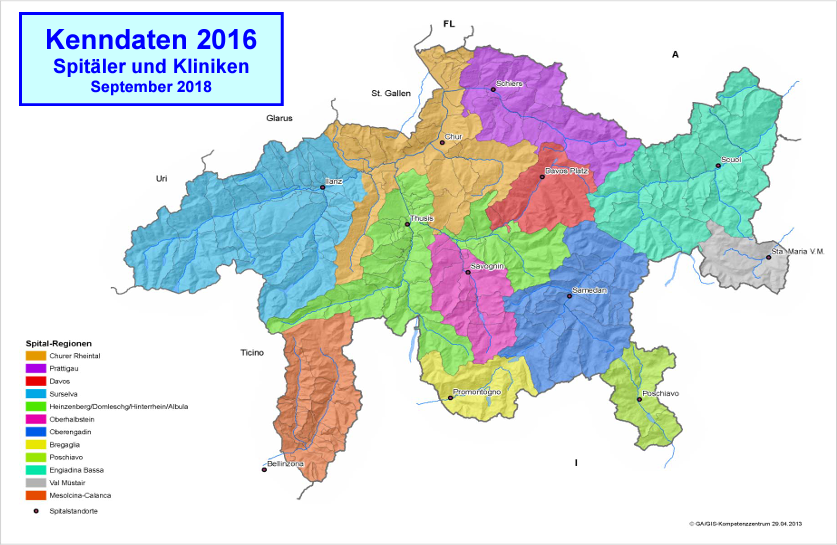
\includegraphics[width=1\linewidth]{source/introduction/initial_situation/gr_spitalregionen}
    \caption{Spitalregionen Kanton Graubünden\cite{ER2J77MB}}
    \label{fig:gr_spitalregionen}
\end{figure}

Seit dem 1. Januar 2023 betreibt das KSGR den Standort Walenstadt im Kanton St. Gallen und deckt primär den Wahlkreis Sarganserland ab.
\begin{figure}[H]
    \centering
    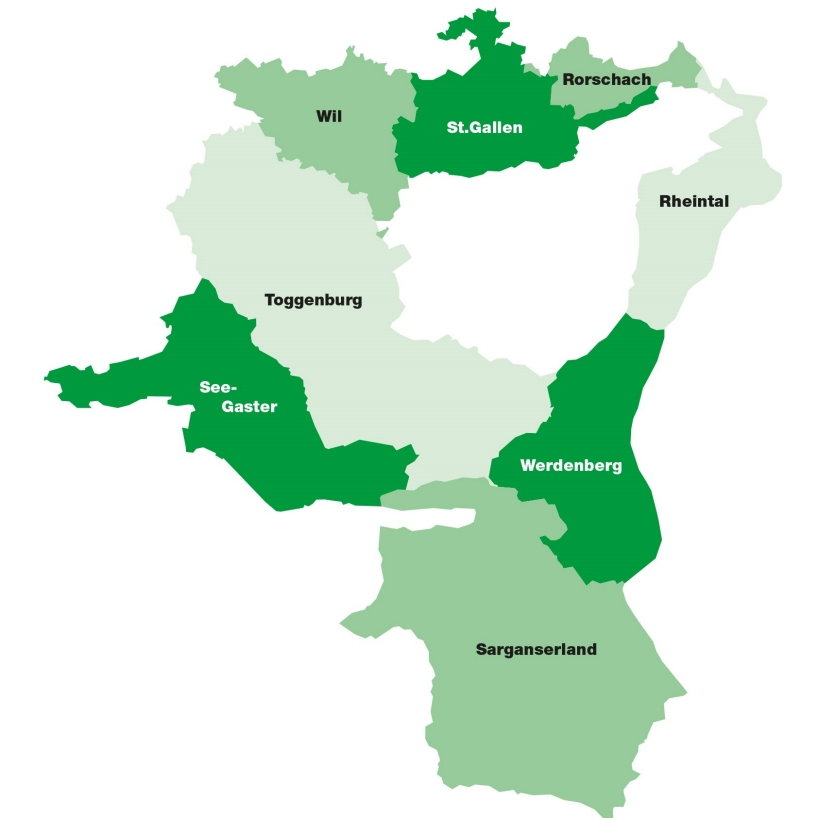
\includegraphics[width=0.75\linewidth]{source/introduction/initial_situation/sg_wahlkreise}
    \caption{Wahlkreise Kanton St. Gallen\cite{LEZ4SPDD}}
    \label{fig:sg_wahlkreise}
\end{figure}

Da dieser Wahlkreis der Spitalregion Rheintal Werdenberg Sarganserland zugeordnet ist, wird das KSGR auch im restlichen südlichen Teil der Spitalregion aktiv sein.
\begin{figure}[H]
    \centering
    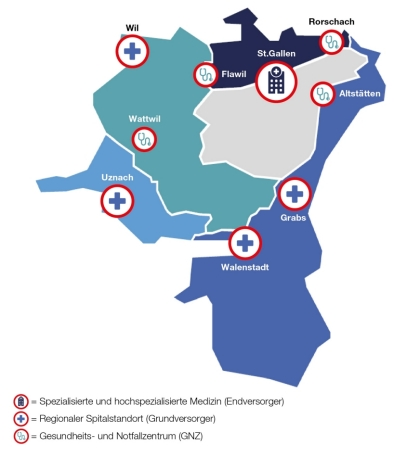
\includegraphics[width=0.5\linewidth]{source/introduction/initial_situation/sg_spitalregionen}
    \caption{Spitalregionen / Spitalstrategie Kanton St. Gallen\cite{3L8EIPUP}}
    \label{fig:sg_spitalregionen}
\end{figure}
\subsection{Die ICT des Kantonsspital Graubünden}
Das Kantonsspital Graubünden hat eine Matrixorganisation.
Die ICT ist ein eigenständiges Departement und gilt als sogenanntes Querschnittsdepartement, dh.
die ICT bedient alle anderen Departemente.
\begin{figure}[H]
    \centering
    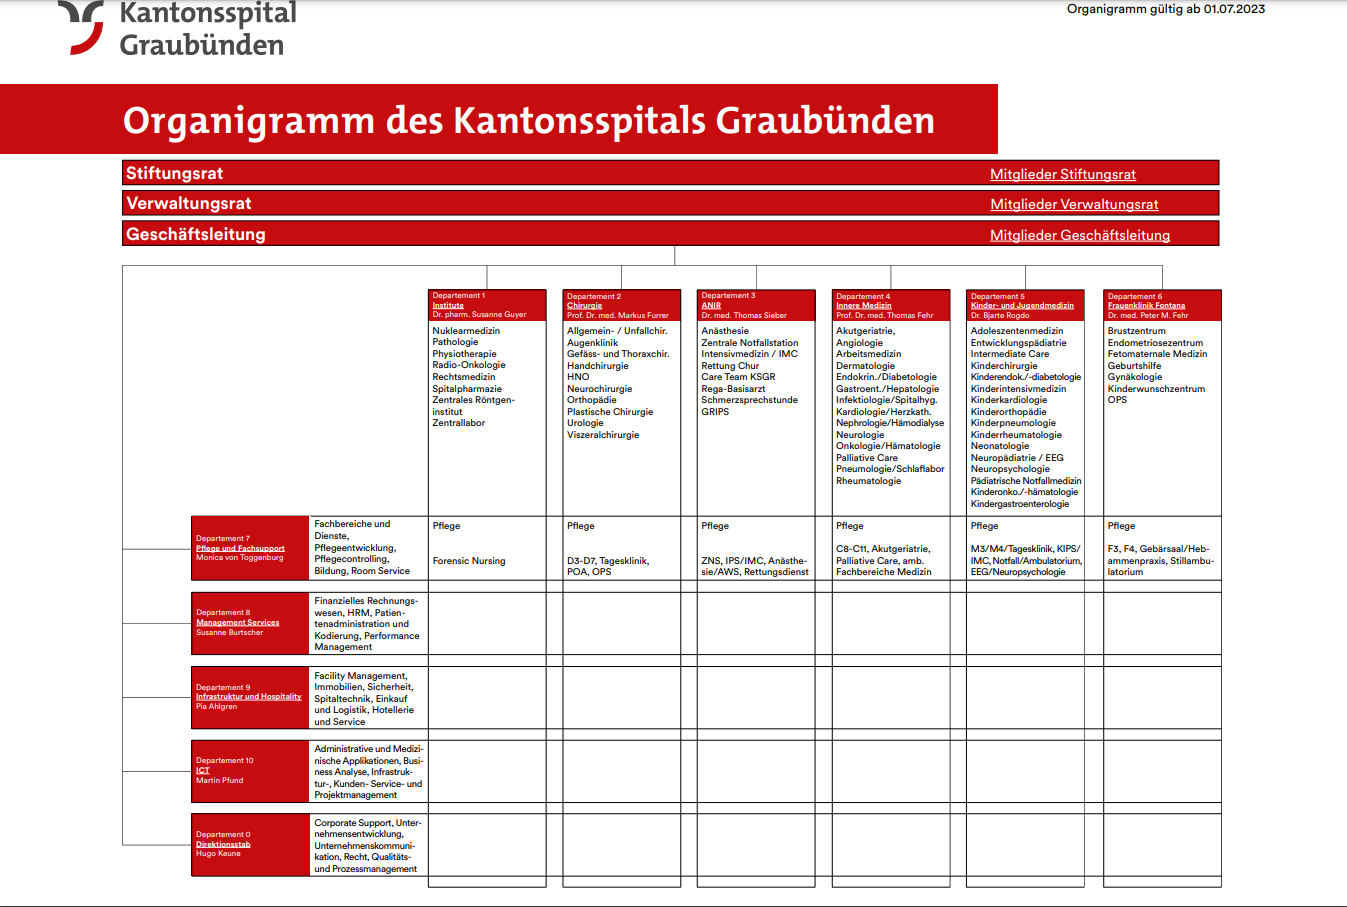
\includegraphics[width=1\linewidth]{source/introduction/initial_situation/Organigramm_KSGR}
    \caption{Organigramm Kantonsspital Graubünden}
    \label{fig:Organigramm_KSGR}
\end{figure}

Die ICT betreibt über 400 Applikationen die auf mehr als 1055 physische und virtuelle Server und Appliances.
Das Rückgrat der Infrastruktur ist dabei die Virtualisierungsplattformen VMware ESXi für Server und Citrix für die Thinclients der Enduser.
Es werden aber auch Dienstleistungen für andere Spitäler und Kliniken oder andere Einrichtungen des Gesundheitswesens erbracht.

Entsprechen wurde die ICT in ein Applikationsmanagement, ein Infrastrukturmanagement sowie einem unterstützenden Bereich aufgegliedert.
Das Applikationsmanagement wurde in je einen Bereich für die Administrativen und Medizinischen Applikationen aufgeteilt.
Das Infrastrukturmanagement wiederum wurde in den Bereich Netzwerk und Data Center, welcher für Server zuständig ist, aufgeteilt.
Der Bereich Business- und Prozessunterstützung beinhaltet je eine Abteilung für die Businessanalyse, das Projektmanagement und Benutzer- und Clientservices in der auch der Service-Desk untergebracht ist.
\begin{figure}[H]
    \centering
    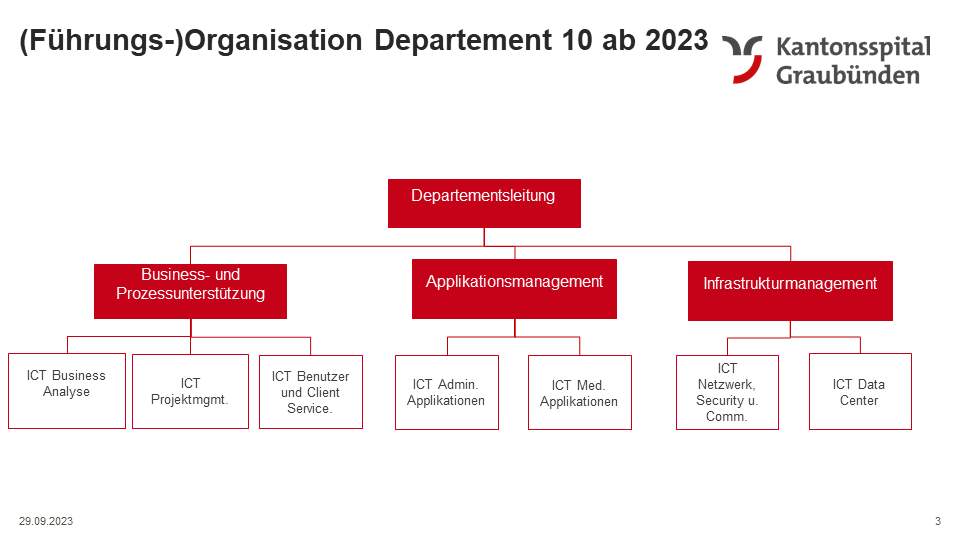
\includegraphics[width=1\linewidth]{source/introduction/initial_situation/Organigramm-D10}
    \caption{Organigramm Departement 10 - ICT}
    \label{fig:Organigramm_D10}
\end{figure}

Die Organisation der ICT wird sich aber bis spätestens zum Abschluss der Diplomarbeit noch verändern.
\subsection{Rolle in der ICT vom Kantonsspital Graubünden}
Meine Rolle im Kantonsspital Graubünden resp. in der ICT ist die eines DBA.
Diese Rolle ist in der Abteilung ICT Data Center.

Da die Kernsysteme auf Oracle Datenbanken und \Gls{HP-UX} laufen, bin ich primär \Gls{Oracle Database} DBA und manage das \Gls{HP-UX} in Zusammenarbeit mit HPE.
Die administrative Tätigkeit bei \Gls{HP-UX} besteht primär im Betrieb der \Gls{HP-UX} Cluster Packages (einer sehr
rudimentären Art von Containern), überwachen und erweitern des Filesystems, erweitern von \Gls{SAN} Storage Lunes für die Filesystem erweiterung, Erstellen von \Gls{PRTG}-Sensoren für
das Monitoring, SAP Printerqueue Management und andere Tasks die es noch auszuführen gibt.
Daneben bin ich auch für andere Datenbanken, teilweise aber nur begrenzt \Gls{Microsoft SQL Server}, \Gls{MySQL} /
\Gls{MariaDB} und vermehrt \Gls{PostgreSQL} zuständig.
Darüber hinaus bin ich Teilweise in die \Gls{Linux}-Administration involviert und betreue auch noch einige Windows Server für das Zentrale klinische Informationssystem.

\subsection{Ausgangslange}
Die meisten der über 400 Applikationen, die das KSGR betreibt, haben in den allermeisten Fällen ihre Daten in Datenbanksysteme speichern.
Entsprechend der Vielfalt der Applikationen existieren auch eine vielzahl an Datenbanksystemen und Versionen.

Basierend auf der Liste \textit{DB-Engines Ranking}\cite{TTVGIG2P} der Top-Datenbanksysteme .
Allerdings werden nicht alle Datenbanksysteme berücksichtigt, entweder weil das Datenbanksystem keine Client/Server Architektur hat oder nicht im Scope der IT oder des Projekts ist.

Folgende Datenbanken sind inventarisiert:
\begin{landscape}
\begin{table}[]
\resizebox{\columnwidth}{!}{%
\begin{tabular}{@{}llll@{}}
\toprule
\textbf{DBMS}                & \textbf{Datenbankmodell} & \textbf{Inventarisiert} & \textbf{Kommentar}                                                            \\ \midrule
\Gls{Oracle Database}                       & Relational, \Gls{NoSQL}, \Gls{OLAP}  & Ja                      &                                                                               \\
\Gls{MySQL}                        & Relational               & Ja                      &                                                                               \\
\Gls{Microsoft SQL Server}         & Relational, \Gls{NoSQL}, \Gls{OLAP}  & Nein                    & Werden separat administriert und sind daher nicht in diesem Inventar gelistet \\
\Gls{PostgreSQL}                   & Relational, \Gls{NoSQL}        & Ja                      &                                                                               \\
\Gls{MongoDB}                      & \Gls{NoSQL}                    & Ja                      &                                                                               \\
\Gls{Redis}                        & Key-value                & Ja                      &                                                                               \\
\Gls{Elasticsearch}                & Search engine            & Ja                      &                                                                               \\
\Gls{IBM DB2}                      & Relational               & Ja                      &                                                                               \\
\Gls{SQLite}                       & Relational               & Nein                    & Lokale Datenbank. Zudem wird die DB nicht via Netzwerk angesprochen           \\
\Gls{Microsoft Access}             & Relational               & Nein                    & Nicht im Scope der ICT                                                        \\
\Gls{Snowflake}                    & Relational               & Ja                      &                                                                               \\
\Gls{Cassandra}                    & Relational               & Ja                      &                                                                               \\
\Gls{MariaDB}                      & Relational               & Ja                      &                                                                               \\
\Gls{Splunk}                       & Search engine            & Ja                      &                                                                               \\
\Gls{Microsoft Azure SQL Database} & Relational, \Gls{NoSQL}, \Gls{OLAP}  & Nein                    & Datenbanken sind nicht On-Premise und somit nicht im Scope                    \\ \bottomrule
\end{tabular}%
}
\caption{Inventarisierte Datenbanksysteme}
\label{tab:Inventarisierte Datenbanksysteme}
\end{table}
\end{landscape}

Folgende Datenbanksysteme sind demnach im KSGR im Einsatz:
\begin{longtable}{@{}lll@{}}
\toprule
\textbf{\Gls{RDBMS}}                   & \textbf{Summe RDBMS / Cluster / CDB / Instance} & \textbf{Summe Databases} \\* \midrule
\endfirsthead
%
\endhead
%
\bottomrule
\endfoot
%
\endlastfoot
%
\Gls{MariaDB}                 & 2                                      & 2               \\
\Gls{MongoDB}                 & 2                                      & 2               \\
\Gls{MySQL}                   & 28                                     & 50              \\
\Gls{Oracle Database}         & 27                                     & 30              \\
\Gls{PostgreSQL}              & 20                                     & 20              \\
\Gls{Redis}                   & 1                                      & 1               \\* \midrule
\textbf{Gesamtergebnis} & \textbf{80}                            & \textbf{105}    \\* \bottomrule
\caption{Datenbankinventar}
\label{Datenbankinventar}
\end{longtable}


%\begin{figure}[H]
%    \centering
%    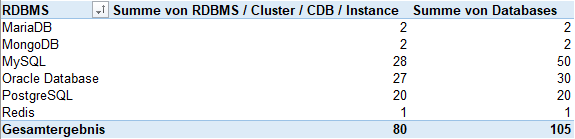
\includegraphics[width=1\linewidth]{source/database_inventory_dbs}
%    \caption{Datenbankinventar}
%    \label{fig:Datenbankinventar}
%\end{figure}

Aufgeschlüsselt auf die Betriebssysteme auf denen die Datenbanken laufen, ergibt sich folgendes Bild:
\begin{longtable}{@{}llrr@{}}
\toprule
\multicolumn{2}{l}{\textbf{OS / \Gls{RDBMS}}}     & \multicolumn{1}{l}{\textbf{Summe RDBMS / Cluster / CDB / Instance}} & \multicolumn{1}{l}{\textbf{Summe Databases}} \\* \midrule
\endfirsthead
%
\endhead
%
\bottomrule
\endfoot
%
\endlastfoot
%
\multicolumn{2}{l}{\textbf{\Gls{HP-UX}}}          & \textbf{21}                                                         & \textbf{24}                                  \\* \midrule
             & \Gls{Oracle Database}s             & 21                                                                  & 24                                           \\
\multicolumn{2}{l}{\textbf{\Gls{Linux}}}          & \textbf{26}                                                         & \textbf{48}                                  \\* \midrule
             & \Gls{MariaDB}                      & 2                                                                   & 2                                            \\
             & \Gls{MySQL}                        & 14                                                                  & 36                                           \\
             & \Gls{Oracle Database}              & 1                                                                   & 1                                            \\
             & \Gls{PostgreSQL}                   & 8                                                                   & 8                                            \\
             & \Gls{Redis}                        & 1                                                                   & 1                                            \\
\multicolumn{2}{l}{\textbf{Windows Server}} & \textbf{33}                                                         & \textbf{33}                                  \\* \midrule
             & \Gls{MongoDB}                      & 2                                                                   & 2                                            \\
             & \Gls{MySQL}                        & 14                                                                  & 14                                           \\
             & \Gls{Oracle Database}s             & 5                                                                   & 5                                            \\
             & \Gls{PostgreSQL}                   & 12                                                                  & 12                                           \\* \midrule
\multicolumn{2}{l}{\textbf{Gesamtergebnis}} & \textbf{80}                                                         & \textbf{105}                                 \\* \bottomrule
\caption{\mbox{Datenbankinventor - Nach Betriebssystemen aufgeschlüsselt}}
\label{Datenbankinventar_per_OS}
\end{longtable}

Die Kernsysteme des Spitals werden auf Oracle Datenbanken (\Gls{Oracle Database})betrieben, die aktuell auf einer \Gls{HP-UX} betrieben werden.
Stand heute gibt es kein Clustersystem für die Open-Source Datenbanken wie \Gls{MariaDB}/\Gls{MySQL} oder \Gls{PostgreSQL}\@.

Durch die Einführung von \Gls{Kubernetes} als Containerplattform wird der Bedarf an \Gls{PostgreSQL} Datenbanken immer grösser.
Es werden in naher Zukunft auch verschiedene Oracle Datenbanken sowie \Gls{MySQL} Datenbanken auf \Gls{PostgreSQL} migriert werden.

Aktuell werden die Daten des \Gls{Zabbix} der Netzwerktechniker auf eine \Gls{MariaDB} Datenbank gespeichert, dies soll sich aber ändern.
Da das \Gls{Zabbix} alle Netzwerkgeräte Überwacht, pro Sekunde werden im Moment 1'200 Datenpunkte abgefragt und xxx in die Datenbank und wird im Laufe der Zeit mehrere Terrabyte gross werden.
\subsection{Problemstellung}
Zusammen mit den bestehenden \Gls{PostgreSQL}-Datenbankinstanzen werden die \Gls{PostgreSQL} Datenbanken in der Art, wie sie bisher Betrieben werden, nicht mehr Betreibbar sein.
Die bisherige Strategie erzeugt sehr viele Aufwände und provoziert Risiken, namentlich:
\begin{itemize}
    \item dezentrale Backups und fragmentierte Backup-Strategien
    \begin{itemize}
        \item Fehlende Kontrolle
        \item Wiederherstellbarkeit nicht garantiert
    \end{itemize}
    \item Verschiedene Betriebssysteme mit verschiedenen Versionen
    \begin{itemize}
        \item Fehlernder Überblick
        \item Veraltete Betriebssystem- und Datenbankversionen
        \item Grosser Administrationsaufwand
    \end{itemize}
    \item Uneinheitliche Absicherung und Härtung
    \begin{itemize}
        \item Hohe Angreifbarkeit
        \item Veraltete Betriebssystem- und Datenbankversionen
        \item Grosser Administrationsaufwand
    \end{itemize}
    \item Uneinheitliche HA-Fähigkeit
    \begin{itemize}
        \item Hohe Angreifbarkeit
        \item Veraltete Betriebssystem- und Datenbankversionen
        \item Grosser Administrationsaufwand
    \end{itemize}
\end{itemize}

Dadurch ergeben sich nach BSI folgende Risiken:
\begin{landscape}
\begin{table}[]
\resizebox{\columnwidth}{!}{%
\begin{tabular}{llllllllllll}
\hline
\multicolumn{4}{l}{}                                                                                                                                                                        &                                                                                                                                                                                                                                                                                                                                                                                                                                                                                                                                                                                                                                                                                                                                                                                                                              &                                                                                                                                                                                                                                                                                                                                                                                                                                                                                                                                                         & \multicolumn{2}{l}{}                                  & \multicolumn{4}{l}{Behandlung}                                                                                                                                                                                                                                 \\ \cline{9-12}
\multicolumn{4}{l}{\multirow{-2}{*}{Identifikation}}                                                                                                                                        & \multirow{-2}{*}{}                                                                                                                                                                                                                                                                                                                                                                                                                                                                                                                                                                                                                                                                                                                                                                                                           & \multirow{-2}{*}{}                                                                                                                                                                                                                                                                                                                                                                                                                                                                                                                                      & \multicolumn{2}{l}{\multirow{-2}{*}{Abschätzung}}     &                                                                                   & \multicolumn{2}{l}{Zielwert} &                                                                                                                                             \\ \cline{1-8} \cline{10-11}
ID & Schutzziel & \begin{tabular}[c]{@{}l@{}}Referenz\\ BSI 200-3\end{tabular} & Risiko                                                                                                     & Beschreibung / Ursache                                                                                                                                                                                                                                                                                                                                                                                                                                                                                                                                                                                                                                                                                                                                                                                                       & Auswirkung                                                                                                                                                                                                                                                                                                                                                                                                                                                                                                                                              & WS                        & SM                        & \multirow{-2}{*}{\begin{tabular}[c]{@{}l@{}}Massnahmen\\ ergreifen?\end{tabular}} & WS            & SM           & \multirow{-2}{*}{Massnahme}                                                                                                                 \\ \hline
1  & I          & G0.22                                                        & Manipulation von Informationen                                                                             & \begin{tabular}[c]{@{}l@{}}Durch veraltete Systeme die zudem unterschiedlich gut gehärtet und \\ gesichert sind (z.B. durch Verschlüsselung des Verkehrs oder der Daten auf dem Storage), \\ besteht das Risiko das Daten manipuliert werden\end{tabular}                                                                                                                                                                                                                                                                                                                                                                                                                                                                                                                                                                    & \begin{tabular}[c]{@{}l@{}}Die Auswirkungen reichen von einer Fehlfunktion des Systems \\ bis hin zum vollständigen Verlust der Integrität der Daten\end{tabular}                                                                                                                                                                                                                                                                                                                                                                                       & \cellcolor[HTML]{F8FF00}2 & \cellcolor[HTML]{F8FF00}4 & Ja                                                                                & 1             & 2            & \begin{tabular}[c]{@{}l@{}}Best-Practice bei Härtung der Systeme.\\ Redundanzen einführen\end{tabular}                                      \\
2  & A          & G0.25                                                        & Ausfall von Geräten oder Systemen                                                                          & \begin{tabular}[c]{@{}l@{}}Manche Datenbanken und deren Betriebssysteme sind sehr alt und sehr lange im Einsatz.\\ Einige dieser Systeme sind schon so alt, das keine Hotfixes,\\ Patches und Updates mehr erhältlich sind.\\ Hierdurch entsteht das Risiko, das Systeme Ausfallen\end{tabular}                                                                                                                                                                                                                                                                                                                                                                                                                                                                                                                              & \begin{tabular}[c]{@{}l@{}}Sofern keine HA-Architektur aufgebaut wurde,\\ ist die Verfügbarkeit ernsthaft gefährdet resp.\\ die Applikation steht nicht mehr zur Verfügung.\end{tabular}                                                                                                                                                                                                                                                                                                                                                                & \cellcolor[HTML]{F8FF00}4 & \cellcolor[HTML]{F8FF00}4 & Ja                                                                                & 2             & 2            & Redundanzen einführen                                                                                                                       \\
3  & C, I, A    & G0.26                                                        & Fehlfunktion von Geräten oder Systemen                                                                     & \begin{tabular}[c]{@{}l@{}}Manche Datenbanken und deren Betriebssysteme sind sehr alt und sehr lange im Einsatz.\\ Einige dieser Systeme sind schon so alt, das keine Hotfixes,\\ Patches und Updates mehr erhältlich sind.\\ Hierdurch entsteht das Risiko, das Systeme Fehlfunktionen erleiden.\\ \\ Allerdings versuchen Datenbanksysteme, die Auswirkungen so gering wie möglich zu halten.\end{tabular}                                                                                                                                                                                                                                                                                                                                                                                                                 & \begin{tabular}[c]{@{}l@{}}Fehlfunktionen können innerhalb von Datenbanksystemen\\ die Datenkonsistenz verletzen,\\ Daten können verloren gehen oder ungewollt von\\ Dritten und unberechtigten Personen eingesehen werden.\\ Systeme könnten nicht mehr oder nur noch eingeschränkt verfügbar werden.\\ \\ Daher sind sowohl Vertraulichkeit, Integrität und Verfügbarkeit gefährdet.\end{tabular}                                                                                                                                                     & 2                         & \cellcolor[HTML]{F8FF00}4 & Ja                                                                                & 2             & 2            & \begin{tabular}[c]{@{}l@{}}Systeme zentralisieren\\ Lifecycle etablieren\end{tabular}                                                       \\
4  & C, I, A    & G0.27-1                                                      & Ressourcenmangel (personelle Ressourcen)                                                                   & \begin{tabular}[c]{@{}l@{}}Aufgrund der sehr heterogenen Landschaft ist der\\ Administrationsaufwand für die jetzigen Systeme sehr gross.\\ Zu gross, als das für jede Datenbank und deren Betriebssystem\\ die notwendige Zeit für eine bedarfsgerechte Administration erbracht werden kann.\\ \\ Dadurch bleiben Fehler länger unentdeckt, Hotfixes, Patches, Updates und Upgrades\\ können nicht oder nicht zur richtigen Zeit eingespielt werden.\\ \\ Bei einem akuten Problemfall ist nicht garantiert,\\ das die Leute erreichbar sind, die notwendig sind\end{tabular}                                                                                                                                                                                                                                               & \begin{tabular}[c]{@{}l@{}}Die Auswirkungen können vielfältig sein,\\ abhängig davon welcher Aspekt unter dem Ressourcenmangel leidet.\\ \\ Grundsätzlich wird aber sowohl die Vertraulichkeit,\\ Integrität und Verfügbarkeit gefährdet.\end{tabular}                                                                                                                                                                                                                                                                                                  & \cellcolor[HTML]{F8FF00}3 & 3                         & Ja                                                                                & 2             & 3            & Systeme zentralisieren                                                                                                                      \\
5  & A          & G0.27-2                                                      & Ressourcenmangel (technische Ressourcen)                                                                   & \begin{tabular}[c]{@{}l@{}}Kann auftreten wenn Ressorucenwachstum zu spät bemerkt wird.\\ So kann die CPU Usage oder das Memory Usage schnell anwachsen.\\ Auch der Storage eines Betriebssystems kann nicht mehr ausreichend für ein System werden.\end{tabular}                                                                                                                                                                                                                                                                                                                                                                                                                                                                                                                                                            & \begin{tabular}[c]{@{}l@{}}Wenn die CPU- und Memory-Usage über einen gewissen Schwellwert geht,\\ fängt das Betriebssystem an zu Priorisieren.\\ Dies wird primär der Endanwender in form von Performance Einbussen bemerken.\\ Im schlimmsten Fall steht eine Anwendung nicht mehr zur Verfügung.\\ \\ Gefährlicher sind Storage Overflows, besonders wenn die Datenbank\\ nicht mehr alle Informationen schreiben konnte,\\ die sie für einen korrekten Neustart benötigte.\\ \\ Doch die folgen bleiben nichtsdesto trotz überschaubar.\end{tabular} & \cellcolor[HTML]{F8FF00}2 & 2                         & Ja                                                                                & 1             & 2            & Monitoring verschärfen                                                                                                                      \\
6  & C, I, A    & G0.31                                                        & \begin{tabular}[c]{@{}l@{}}Fehlerhafte Nutzung oder Administration\\ von Geräten und Systemen\end{tabular} & \begin{tabular}[c]{@{}l@{}}Durch die Vielfalt an Datenbankversionen und Betriebssystemen und\\ Plattformen worauf diese betrieben werden,\\ besteht allen voran das Risiko einer Fehlerhafter Administration und Konfiguration.\end{tabular}                                                                                                                                                                                                                                                                                                                                                                                                                                                                                                                                                                                 & \begin{tabular}[c]{@{}l@{}}Abhängig davon, welche Fehler gemacht wurden können\\ die Auswirkungen auch stark variieren.\\ Sie reichen von fehlender Verschlüsselung bis hin zu nicht vorhandenem\\ Backup mit nicht mehr gesicherter Wiederherstellbarkeit von Systemen.\\ \\ Daraus erschliesst sich das auch bei diesem Risiko die Vertraulichkeit,\\ Integrität und Verfügbarkeit gefährdet ist.\end{tabular}                                                                                                                                        & \cellcolor[HTML]{F8FF00}4 & 3                         & Ja                                                                                & 2             & 3            & Systeme zentralisieren                                                                                                                      \\
7  & C, I, A    & G0.32                                                        & Missbrauch von Berechtigungen                                                                              & \begin{tabular}[c]{@{}l@{}}Obwohl das Microsoft Active Directory die Zentrale Benutzerverwaltung ist,\\ sind die wenigsten Datenbanken an dieses angeschlossen.\\ Hinzu kommt der umstand, das in der Vergangenheit jeder Softwarelieferant\\ sein eigenes Benutzerkonzept mitgebracht hat,\\ auch bei den Datenbankzugängen.\\ \\ Multipliziert mit der Anzahl der unterschiedlichsten Datenbanken,\\ Betriebssystemen und Applikationen entsteht das Risiko,\\ das Berechtigungen Wissendlich oder Unwissendlich missbraucht werden.\end{tabular}                                                                                                                                                                                                                                                                          & \begin{tabular}[c]{@{}l@{}}Der Wissentliche oder Unwissentliche Missbrauch von Berechtigungen\\ kann verheerende Auswirkungen haben.\\ Unter anderem können Daten missbräuchlich abgezogen werden,\\ Daten manipuliert oder das ganze System komplett zerstört werden.\end{tabular}                                                                                                                                                                                                                                                                     & 2                         & \cellcolor[HTML]{F8FF00}4 & Ja                                                                                & 2             & 2            & \begin{tabular}[c]{@{}l@{}}Systeme zentralisieren\\ \\ Übergreifendes Berechtigungskonzept einführen\\ Monitoring der Zugriffe\end{tabular} \\
8  & A, I       & G0.45                                                        & Datenverlust                                                                                               & \begin{tabular}[c]{@{}l@{}}Verschiedene Datenbanken sind Standalone Cluster (Instanzen)\\ welche über keinen Failover-Mechanismus verfügen.\\ \\ Zudem wurden die meisten Datenbanken nur mittels Snapshots oder einem\\ Filesystem Backup gesichert, nicht über eine eigentliche Sicherung mittels WAL.\\ Gerade die fehlende WAL-Archivierung führt im Backupfall dazu,\\ das alle Transaktionen die zwischen dem letzten Backup nicht mehr vorhanden sind.\\ \\ Hinzu kommt, das für die meisten Datenbanken hohe Sicherungsintervalle\\ von einmal pro Stunde oder gar nur einmal  am Tag gewählt wurde.\\ \\ Ein weiterer Aspekt des Risikos besteht in der tatsache,\\ das aufgrund der grossen Anzahl Datenbanken und deren\\ Heterogenität nur wenige Backups auch wirklich regelmässig geprüft werden.\end{tabular} & \begin{tabular}[c]{@{}l@{}}Aus dem Risiko ergeben sich zwei Auswirkungen,\\ die aber beide ein hohes Mass an Schaden verursachen können.\\ \\ Erstens könnten Backups gar nicht mehr Wiederhergestellt werden,\\ dies hätte dann einen Totalen Datenverlust zur Folge.\\ Die zweite Ursache erwächst auf der fehlenden WAL-Archivierung,\\ dadurch können zwar die Daten bis zu einem Zeitpunkt X Wiederhergestellt\\ werden allerdings sind diese dann nicht zwingend Konsistent.\end{tabular}                                                         & \cellcolor[HTML]{F8FF00}4 & \cellcolor[HTML]{F8FF00}5 & Ja                                                                                & 1             & 3            & \begin{tabular}[c]{@{}l@{}}Systeme zentralisieren\\ Einheitliches Backupkonzept\\ Regelmässige Restore-Tests\end{tabular}                   \\ \cline{5-12}
\end{tabular}%
}
\caption{Risiko-Matrix aktuelle Situation PostgreSQL Datenbanken}
\label{tab:riskmatrix-postgresql}
\end{table}
\end{landscape}

\begin{figure}[H]
    \centering
    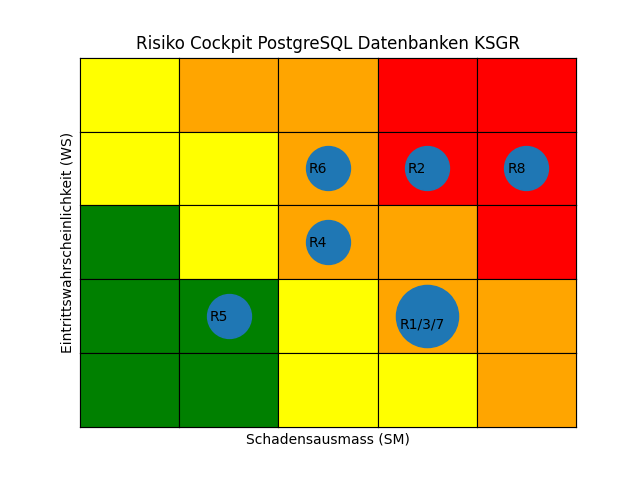
\includegraphics[width=1\linewidth]{source/riskmatrix/riskmatrixproblem}
    \caption{Risiken bestehende Lösung}
    \label{fig:riskmatrixproblem}
\end{figure}

% Python matplot risk management => versuchen
%https://stackoverflow.com/questions/62154079/risk-matrix-with-pythyon

Daraus ergeben sich folgende Strategien und Handlungsfelder um die Massnahmen zur Risikominimierung umzusetzen:
\begin{itemize}
    \item Systemabsicherung erarbeiten und einsetzen
    \item HA-Clustering einführen um die Redundanz zu gewährleisten und Systeme zentral verwalten und betreiben zu können
    \item Lifecycle-management für Datenbanken und Betriebssysteme erarbeiten und einsetzen
    \item Backupkonzept erarbeiten
    \item Berechtigungskonzept erarbeiten und einführen
\end{itemize}

Mit diesen Massnahmen lassen sich die Risiken gesenkt werden:
\begin{figure}[H]
    \centering
    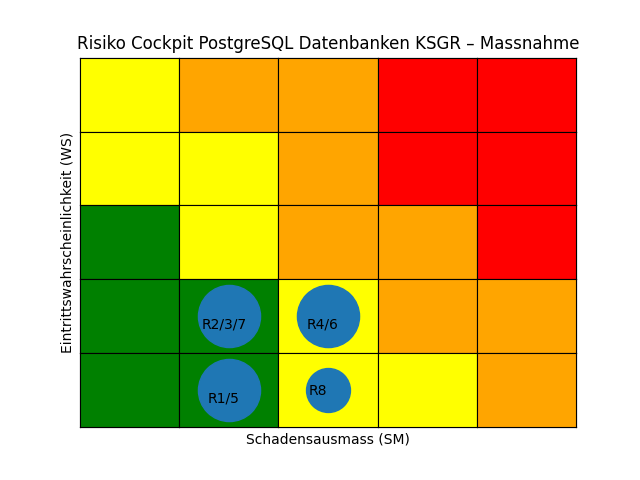
\includegraphics[width=1\linewidth]{source/riskmatrix/Riskmatrixproblem-massnahmen}
    \caption{Risiken bestehende Lösung mit Massnahmen}
    \label{fig:riskmatrixproblem-massnahmen}
\end{figure}
    %! Author = itgramic
%! Date = 29.09.23

% Preamble
%\newpage
%\begin{landscape}
%\begin{flushleft}
\clearpage
%    \KOMAoptions{paper=A3,paper=landscape,pagesize}
\KOMAoptions{paper=A3,paper=landscape,pagesize, DIV=20}
\recalctypearea
\section{Zieldefinition}
%\begin{flushleft}
Das administrieren einer \Gls{PostgreSQL} Datenbank umfasst i.d.R. \cite{5TA9H3I4,IFLSFQU4} folgende zehn Tasks die zum täglichen Alltag gehören:
%\end{flushleft}
\begin{table}[H]
\resizebox{\columnwidth}{!}{%
\begin{tabular}{@{}llll@{}}
\toprule
\textbf{Nr.} & \textbf{Aufgabe}                                                                   & \textbf{Beschreibung}                                                                                                                                                                                                                                                                                                                                                                                                                                                 & \textbf{Wichtigkeit} \\ \midrule
1            & Failover                                                                           & In einem Fehlerfall soll die DB-Node auf einen Standby-Node übergeben werden.                                                                                                                                                                                                                                                                                                                                                                                         & Hoch                 \\
2            & Failover Restore                                                                   & \begin{tabular}[c]{@{}l@{}}Nach einem Failover muss der DB-Node wieder vom Standby-Node auf den Primären Node zurückgesetzt werden.\\ Dabei darf es zu keinem Datenverlust kommen, also alle Daten die auf dem Standby-Node erfasst wurden, \\ müssen auf den Primären DB-Node zurückgeschrieben werden beim Failover Restore\end{tabular}                                                                                                                            & Hoch                 \\
3            & Filesystem Management                                                              & \begin{tabular}[c]{@{}l@{}}Die Datenmenge von Datenbanken wachsen in der Regel beständig.\\ Die Belegung von Tablespaces und Filesystem muss deshalb Überwacht und ggf. erweitert werden.\\ Läuft eine Disk voll kommt es im besten Fall zu einem Stillstand der DB, im schlimmsten Fall zu Inkonsistenzen und Datenverlust\end{tabular}                                                                                                                              & Hoch                 \\
4            & Monitoring                                                                         & \begin{tabular}[c]{@{}l@{}}Nebst den allgemeinen Metriken wie CPU / Memory Usage und der Port Verfügbarkeit gibt es noch eine reihe weiterer Aspekte die Überwacht werden müssen.\\ Zum Beispiel ob es zu verzögerungen bei der Replikation kommt oder die Tablespaces genügend Platz haben.\\ Dazu gehört auch das Überwachen des Logs und entsprechende Schritte im Fehlerfall.\end{tabular}                                                                        & Mittel               \\
5            & Statistiken / Cleanup Jobs justieren                                               & \begin{tabular}[c]{@{}l@{}}\Gls{PostgreSQL} sammelt Statistiken um SQL Queries optimaler ausführen zu können. \\ Zudem wird im Rahmen des gleichen Sheduled Tasks ein Cleanup Vorgenommen, \\ so dass z.B. gelöschte Datensätze den Disk Space nicht sinnlos belegen.\\ Die Konfiguration dieser Jobs muss an der Metrik der Datenbank angepasst werden, \\ weil gewisse Tasks dann entweder viel zu oft oder viel zu wenig bis gar nicht mehr ausgeführt werden.\end{tabular} & Mittel               \\
6            & SQL optimierungen                                                                  & \begin{tabular}[c]{@{}l@{}}In \Gls{PostgreSQL} können inperfomante SQL Statements ausgelesen werden und zum Teil werden auch informationen zum Tuning geliefert\cite{RJFW5WUH}.\\ Diese müssen Regelmässig ausgelesen werden\end{tabular}                                                                                                                                                                                                                                                  & Tief                 \\
7            & \begin{tabular}[c]{@{}l@{}}Health Checks und Aktionen\\ (Maintenance)\end{tabular} & \begin{tabular}[c]{@{}l@{}}Regelmässig muss die Gesundheit der DBs überprüft werden, etwa ob Tabellen und/oder Indizes sich aufgebläht haben oder ob Locks vorhanden sind\cite{DPBK2HT5}.\\ Während der Hauptarbeitszeit muss dies mindestens alle 90 Minuten geprüft und ggf. reagiert werden.\end{tabular}                                                                                                                                                                         & Hoch                 \\
8            & Housekeeping                                                                       & \begin{tabular}[c]{@{}l@{}}Mit Housekeeping Jobs werden regelmässig Trace- und Alertlogfiles aufgeräumt, \\ um Platz auf den Disken zu sparen aber auch um die Übersichtlichkeit zu wahren.\end{tabular}                                                                                                                                                                                                                                                              & Mittel               \\
9            & Verwalten von DB Objekten                                                          & \begin{tabular}[c]{@{}l@{}}Regelmässig müssen DB Objekte wie Datenbanken, Tabellen, Trigger, Views etc. angepasst oder erstellt werden.\\ Dies richtet sich nach den Bedürfnis der Kunden resp. deren Applikationen.\end{tabular}                                                                                                                                                                                                                                     & Tief                 \\
10           & User Management                                                                    & \begin{tabular}[c]{@{}l@{}}Die Zugriffe der User müssen Überwacht, angepasst, erfasst oder gesperrt werden.\\ Auch diese Aufgabe richtet sich nach den Bedürfnissen der Kunden.\end{tabular}                                                                                                                                                                                                                                                                          & Tief                 \\ \bottomrule
\end{tabular}%
}
\caption{Administrative Aufgaben}
\label{tab:administrative_aufgaben}
\end{table}
%\begin{flushleft}
\clearpage
%    \KOMAoptions{paper=A3,paper=landscape,pagesize}
\KOMAoptions{paper=A3,paper=landscape,pagesize, DIV=20}
\recalctypearea
Von diesen Tasks müssen Teile davon zu 50\% automatisiert werden wobei alle Muss-Aufgaben automatisiert werden müssen.
Diese wären nachfolgende Tasks die automatisiert werden können.
%\end{flushleft}

%\newpage
%\begin{flushleft}
%\clearpage
%%    \KOMAoptions{paper=A3,paper=landscape,pagesize}
%\KOMAoptions{paper=A3,paper=landscape,pagesize, DIV=20}
%\recalctypearea
%\end{landscape}
%\begin{landscape}
\begin{table}[H]
\resizebox{\columnwidth}{!}{%
\begin{tabular}{@{}lllllll@{}}
\toprule
\textbf{Nr.} & \textbf{Aufgabe}                                                                   & \textbf{Wichtigkeit} & \textbf{Zu automatisierender Task}                                                                                                                                                                                                                                                                                                                                                              & \textbf{Priorität} & \textbf{Muss / Kann} & \textbf{Spätester Termin} \\ \midrule
1            & Failover                                                                           & Hoch                 & Automatisierter Failover auf mindestens einen Sekundären DB-Node                                                                                                                                                                                                                                                                                                                                & 1                  & Muss                 & Abgabe                    \\
2            & Failover Restore                                                                   & Hoch                 & \begin{tabular}[c]{@{}l@{}}Sobald der Primäre DB-Node wieder vorhanden ist,\\ muss automatisch auf den Primären DB-Node zurückgesetzt werden.\end{tabular}                                                                                                                                                                                                                                      & 1                  & Muss                 &                           \\
3            & Filesystem Management                                                              & Hoch                 & \begin{tabular}[c]{@{}l@{}}Das Filesystem muss beim erreichen von 95\% Usage automatisiert vergrössert werden.\\ Die Vergrösserung muss anhand der Wachstumsrate (die mittels Linux Commands zu ermitteln ist),\\ vergrössert werden\end{tabular}                                                                                                                                               & 4                  & Kann                 &                           \\
4            & Monitoring                                                                         & Mittel               & Der Status der Clusterumgebung und der Replikation muss im \Gls{PRTG} überwacht werden                                                                                                                                                                                                                                                                                                                & 2                  & Muss                 &                           \\
5            & Statistiken / Cleanup Jobs justieren                                               & Mittel               & \begin{tabular}[c]{@{}l@{}}Regelmässig müssen die Parameter für den \Gls{AUTOVACUUM} Job berechnet werden und\\ das Configfile postgresql.conf automatisch angepasst werden\end{tabular}                                                                                                                                                                                                              & 2                  & Muss                 &                           \\
6            & SQL optimierungen                                                                  & Tief                 & \begin{tabular}[c]{@{}l@{}}Es gibt SQL Abfragen, mit dem fehlende Indizes ermittelt werden können.\\ Diese Indizes sollen automatisiert erstellt werden.\\ \\ Im gleichen Zug sollen aber auch Indizes, welche nicht verwendet werden, entfernt werden.\\ Sie tragen nicht nur nichts zu performanteren Abfragen bei\\ sondern beziehen unnötige Ressourcen bei Datenmanipulationen\cite{RJFW5WUH}.\end{tabular} & 2                  & Kann                 &                           \\
7            & \begin{tabular}[c]{@{}l@{}}Health Checks und Aktionen\\ (Maintenance)\end{tabular} & Hoch                 & \begin{tabular}[c]{@{}l@{}}Tabellen und Indizes können sich aufblähen (bloaded table / bloaded index)\\ Ist ein Index aufgebläht, kann dies mittels eines REINDEX\\ mit geringem Impact auf die Datenbank gelöst werden\cite{DPBK2HT5}.\end{tabular}                                                                                                                                                            & 2                  & Muss                 &                           \\
8            & Housekeeping                                                                       & Mittel               & Log Rotation muss aktiviert werden und alte Logs regelmässig gelöscht werden.                                                                                                                                                                                                                                                                                                                   & 3                  & Kann                 &                           \\
9            & Verwalten von DB Objekten                                                          & Tief                 & Keine automatisierung möglich                                                                                                                                                                                                                                                                                                                                                                   & 5                  &                      &                           \\
10           & User Management                                                                    & Tief                 & Regelmässige Reports sollen User aufzeigen, die seit mehr als einer Woche nicht mehr aktiv waren.                                                                                                                                                                                                                                                                                               & 4                  & Kann                 &                           \\ \bottomrule
\end{tabular}%
}
\caption{Automatisierung Administrativer Aufgaben}
\label{tab:automatgisierung_administrative_aufgaben}
\end{table}
%\end{flushleft}
%\end{landscape}
%\begin{flushleft}
Mit der Arbeit sollen folgende Ergebnisse und Resultate erzielt werden:
\begin{itemize}
    \item Ergebnisse \\ Mindestens drei Methoden einen \Gls{PostgreSQL Cluster} aufzubauen müssen analysiert und evaluirt werden
    \item Resultate \\ Aus den mindestens drei Methoden muss die optimale Methode ermittelt werden. \\ Am Ende muss zudem ein Funktionierendes Testsystem bestehen.
\end{itemize}
%\end{flushleft}
%\begin{flushleft}

%\end{flushleft}
%\begin{flushleft}
\clearpage
%    \KOMAoptions{paper=A3,paper=landscape,pagesize}
\KOMAoptions{paper=A3,paper=landscape,pagesize, DIV=15}
\recalctypearea
Daraus ergeben sich folgende Ziele:
%\begin{landscape}
\begin{table}[H]
\resizebox{\columnwidth}{!}{%
\begin{tabular}{@{}llll@{}}
\toprule
\textbf{Nr.} & \textbf{Ziel}                                     & \textbf{Beschreibung}                                                                                                                                                                                                                                                                                                                                                                                                                                                                                                                                                                                                                                                                                                                                                                                                                                                                & \textbf{Priorität} \\ \midrule
1            & Evaluation                                        & \begin{tabular}[c]{@{}l@{}}Am Ende der Evaluationsphase müssen mindestens drei Methoden für einen \Gls{PostgreSQL HA Cluster} müssen evaluirt werden.\\ Innerhalb der evaluation muss analysiert werden, welche Methode oder welches Tool sich hierfür eignen würde.\end{tabular}                                                                                                                                                                                                                                                                                                                                                                                                                                                                                                                                                                                   & Hoch               \\
2            & Testsystem                                        & Am Ende der Diplomarbeit muss ein funktionierendes Testsystem Installiert sein.                                                                                                                                                                                                                                                                                                                                                                                                                                                                                                                                                                                                                                                                                                                                                                                                      & Hoch               \\
3            & Automatisierter Failover                          & \begin{tabular}[c]{@{}l@{}}Ein \Gls{PostgreSQL Cluster} muss im Fehlerfall auf mindestens einen Standby-Node umschwenken.\\ Dabei muss das Timeout so niedrig sein, dass Applikationen nicht auf ein Timeout laufen.\end{tabular}                                                                                                                                                                                                                                                                                                                                                                                                                                                                                                                                                                                                                                   & Hoch               \\
4            & Automatisierter Failover Restore                  & Nach einem Failover muss es zu einem Fallback oder Failover Restore kommen, sobald der Primary-Node wieder verfügbar ist.                                                                                                                                                                                                                                                                                                                                                                                                                                                                                                                                                                                                                                                                                                                                                            & Hoch               \\
5            & Monitoring - Cluster Healthcheck                  & \begin{tabular}[c]{@{}l@{}}Die wichtigsten Parameter für das Monitoring des \Gls{PostgreSQL Cluster}s (isready, Locks, bloaded Tables), \\ der Replikation (Replay Lag, Standby alive) und des \Gls{PostgreSQL HA Cluster}s müssen Überwacht werden.\end{tabular}                                                                                                                                                                                                                                                                                                                                                                                                                                                                                                                                                                                  & Mittel             \\
6            & \Gls{AUTOVACUUM} - Parameter verwalten                  & \begin{tabular}[c]{@{}l@{}}Täglich müssen die Parameter für den \Gls{AUTOVACUUM} Job berechnet werden und\\ das Configfile postgresql.conf automatisch angepasst werden\end{tabular}                                                                                                                                                                                                                                                                                                                                                                                                                                                                                                                                                                                                                                                                                                       & Mittel             \\
7            & SQL optimierungen - Indizes tracken und verwalten & Täglich fehlende Indizes automatisiert erstellen und nicht mehr verwendete Indizes automatisiert entfernen                                                                                                                                                                                                                                                                                                                                                                                                                                                                                                                                                                                                                                                                                                                                                                           & Mittel             \\
8            & Maintenance - Indizes säubern                     & Täglich bloaded Indices, also aufgeblähte Indizes, automatisiert erkennen und mittels REINDEX bereinigen                                                                                                                                                                                                                                                                                                                                                                                                                                                                                                                                                                                                                                                                                                                                                                             & Hoch               \\
9            & Housekeeping - Log Rotation                       & Die Log Rotation muss aktiviert werden. Die Logs müssen aber auch in das KSGR-Log Repository geschrieben werden                                                                                                                                                                                                                                                                                                                                                                                                                                                                                                                                                                                                                                                                                                                                                                      & Hoch               \\
10           & User Management - Monitoring                      & Nicht verwendete User sollen einmal pro Woche automatisiert erkannt und in einem Report gemeldet werden.                                                                                                                                                                                                                                                                                                                                                                                                                                                                                                                                                                                                                                                                                                                                                                             & Tief               \\
11           & Evaluationsziel                                   & Am Ende der Evaluationsphase muss ein Entscheid getroffen worden sein, welche Methode verwendet wird.                                                                                                                                                                                                                                                                                                                                                                                                                                                                                                                                                                                                                                                                                                                                                                                & Hoch               \\
12           & Installationsziel                                 & Die Testinstallation muss Lauffähig sein und zudem alle Anforderungen und Ziele (3 und 4) erfüllen                                                                                                                                                                                                                                                                                                                                                                                                                                                                                                                                                                                                                                                                                                                                                                                   & Hoch               \\
13           & Testziele                                         & \begin{tabular}[c]{@{}l@{}}Folgende Testziele müssen erreicht werden:\\ 1. Der \Gls{PostgreSQL Cluster} muss immer Lauffähig sein solange noch ein Node up ist, unabhängig davon welche Nodes des \Gls{PostgreSQL HA Cluster}s down ist\\ 2. Ein Switchover auf alle Secondary Nodes muss möglich sein\\ 3. Der Fallback auf den Primary Node muss Erfolgreich sein, unabhängig davon ob ein Failover oder \Gls{Switchover} stattgefunden hat\\ 4. Das Timeout bei einem \Gls{Failover} / \Gls{Switchover} muss unterhalb der Default Timeouts der Applikationen \Gls{GitLab} und \Gls{Harbor} liegen.\\ 5. Das Replay Lag zwischen Primary und Secondary darf beim Initialen Start nicht über eine Minute dauern oder 1KiB nicht überschreiten\end{tabular} & Hoch               \\ \bottomrule
\end{tabular}%
}
\caption{Ziele}
\label{tab:ziele}
\end{table}
%\end{landscape}
%\clearpage
%\KOMAoptions{paper=A4,paper=portrait,pagesize}
%\recalctypearea
%\end{flushleft}
%\clearpage
%\KOMAoptions{paper=A4,paper=portrait,pagesize}
%\recalctypearea

    %! Author = itgramic
%! Date = 29.09.23

% Preamble
%\begin{longtable}{@{}lll@{}}
%\toprule
%\textbf{System}                            & \textbf{Produkt}                       & \textbf{Beschreibung}                                                                                    \\* \midrule
%\endfirsthead
%%
%\endhead
%%
%\bottomrule
%\endfoot
%%
%\endlastfoot
%%
%Storage                                    & HPE 3PAR 8450 SAN Storage System       &                                                                                                          \\
%Virtualisierungsplattform                  & VMware® vSphere®                       &                                                                                                          \\
%Primäres Backupsystem                      & VEEAM Backup System                    &                                                                                                          \\
%provisioning / lifecycle management system & Foremann                               & Ist zurzeit nur für Linux angedacht                                                                                                         \\
%Primäre Linux Distribution                 & Debian                                 & RedHat Enterprise Linux oder Oracle Linux wird nur eingesetzt, wenn es nicht anders möglich ist          \\
%Primäres Monitoring System                 & Paessler Router Traffic Grapher (PRTG) & Die Netzwerktechnik nutzt Zabbix                                                                         \\
%Container-Plattform                        & Kubernetes                             &                                                                                                          \\
%Infrastructure as code (Iac) System        & Ansible und Terraform                  & Ansible wird von Foremann verwendet, Terraform wird für die Steuerung der Kubernetes-Plattform verwendet \\
%Usermanagement                             & Microsoft Active Directory             &                                                                                                          \\* \bottomrule
%\caption{Gegebene Systeme}
%\label{gegebene_systeme}
%\end{longtable}
%\newpage
\clearpage
\KOMAoptions{paper=A3,paper=landscape,pagesize,DIV=20}
\recalctypearea
%\begin{landscape}
%    \section{Abgrenzungen}
%    \subsection{Gegegene Systeme}
    \begin{flushleft}
    Im Kantonsspital Graub\"unden sind bereits einige Systeme im Einsatz, die gegeben sind.
    \end{flushleft}
    \begin{table}[H]
    \resizebox{\columnwidth}{!}{%
    \begin{tabular}{lll}
    \hline
    \textbf{}                                 & \textbf{Produkt}                                                                            & \textbf{Beschreibung}                                                                                                                                 \\ \hline
    Storage                                   & HPE 3PAR 8450 \Gls{SAN} Storage System                                                            &                                                                                                                                                       \\
    Virtualisierungsplattform                 & VMware® vSphere®                                                                            &                                                                                                                                                       \\
    Prim\"ares Backupsystem                     & VEEAM Backup System                                                                         &                                                                                                                                                       \\
    Provisioning / lifecycle management system & \Gls{Foreman}                                                                                     & Ist zurzeit nur für Linux angedacht                                                                                                                   \\
    Prim\"are Linux Distribution                & \Gls{Debian}                                                                                      &                                                                                                                                                       \\
    Sekund\"are Linux Distributionen            & \begin{tabular}[c]{@{}l@{}}\Gls{Rocky Linux}\\ \Gls{Oracle Linux}\\ RedHat Enterprise Linux (\Gls{RHEL})\end{tabular} & \begin{tabular}[c]{@{}l@{}}RedHat Enterprise Linux (\Gls{RHEL}), \Gls{Rocky Linux} oder \Gls{Oracle Linux} wird nur eingesetzt,\\ wenn es nicht anders möglich ist\end{tabular} \\
    Primäres Monitoring System                & Paessler Router Traffic Grapher (\Gls{PRTG})                                                      & Monitoring System für alle ausser dem Netzwerkbereich                                                                                                 \\
    Sekundäres Monitoring System              & \Gls{Zabbix}                                                                                      & Wird nur vom Netzwerkbereich verwendet                                                                                                                \\
    Container-Plattform                       & \Gls{Kubernetes}                                                                                  &                                                                                                                                                       \\
    Infrastructure as code (Iac) System       & \Gls{Ansible} und \Gls{Terraform}                                                                       & \begin{tabular}[c]{@{}l@{}}\Gls{Ansible} wird von \Gls{Foreman} verwendet, \Gls{Terraform} wird für die Steuerung der \\ \Gls{Kubernetes}-Plattform verwendet\end{tabular}   \\
    Logplattform / \Gls{SIEM} System                &                                                                                             & \begin{tabular}[c]{@{}l@{}}Wird neu Ausgeschrieben.\\ Produkt zurzeit nicht definiert\end{tabular}                                                    \\
    Usermanagement                            & Microsoft Active Directory                                                                  &                                                                                                                                                       \\ \hline
    \end{tabular}%
    }
    \caption{Gegebene Systeme}
    \label{tab:gegebene_systeme}
    \end{table}

    %\end{landscape}
    \begin{flushleft}
    Daraus ergeben sich nach nach Z\"ust, Troxler 2002\cite{EDGTQIKU} folgende Abgrenzungen:
    \end{flushleft}
    \begin{figure}[H]
        \centering
        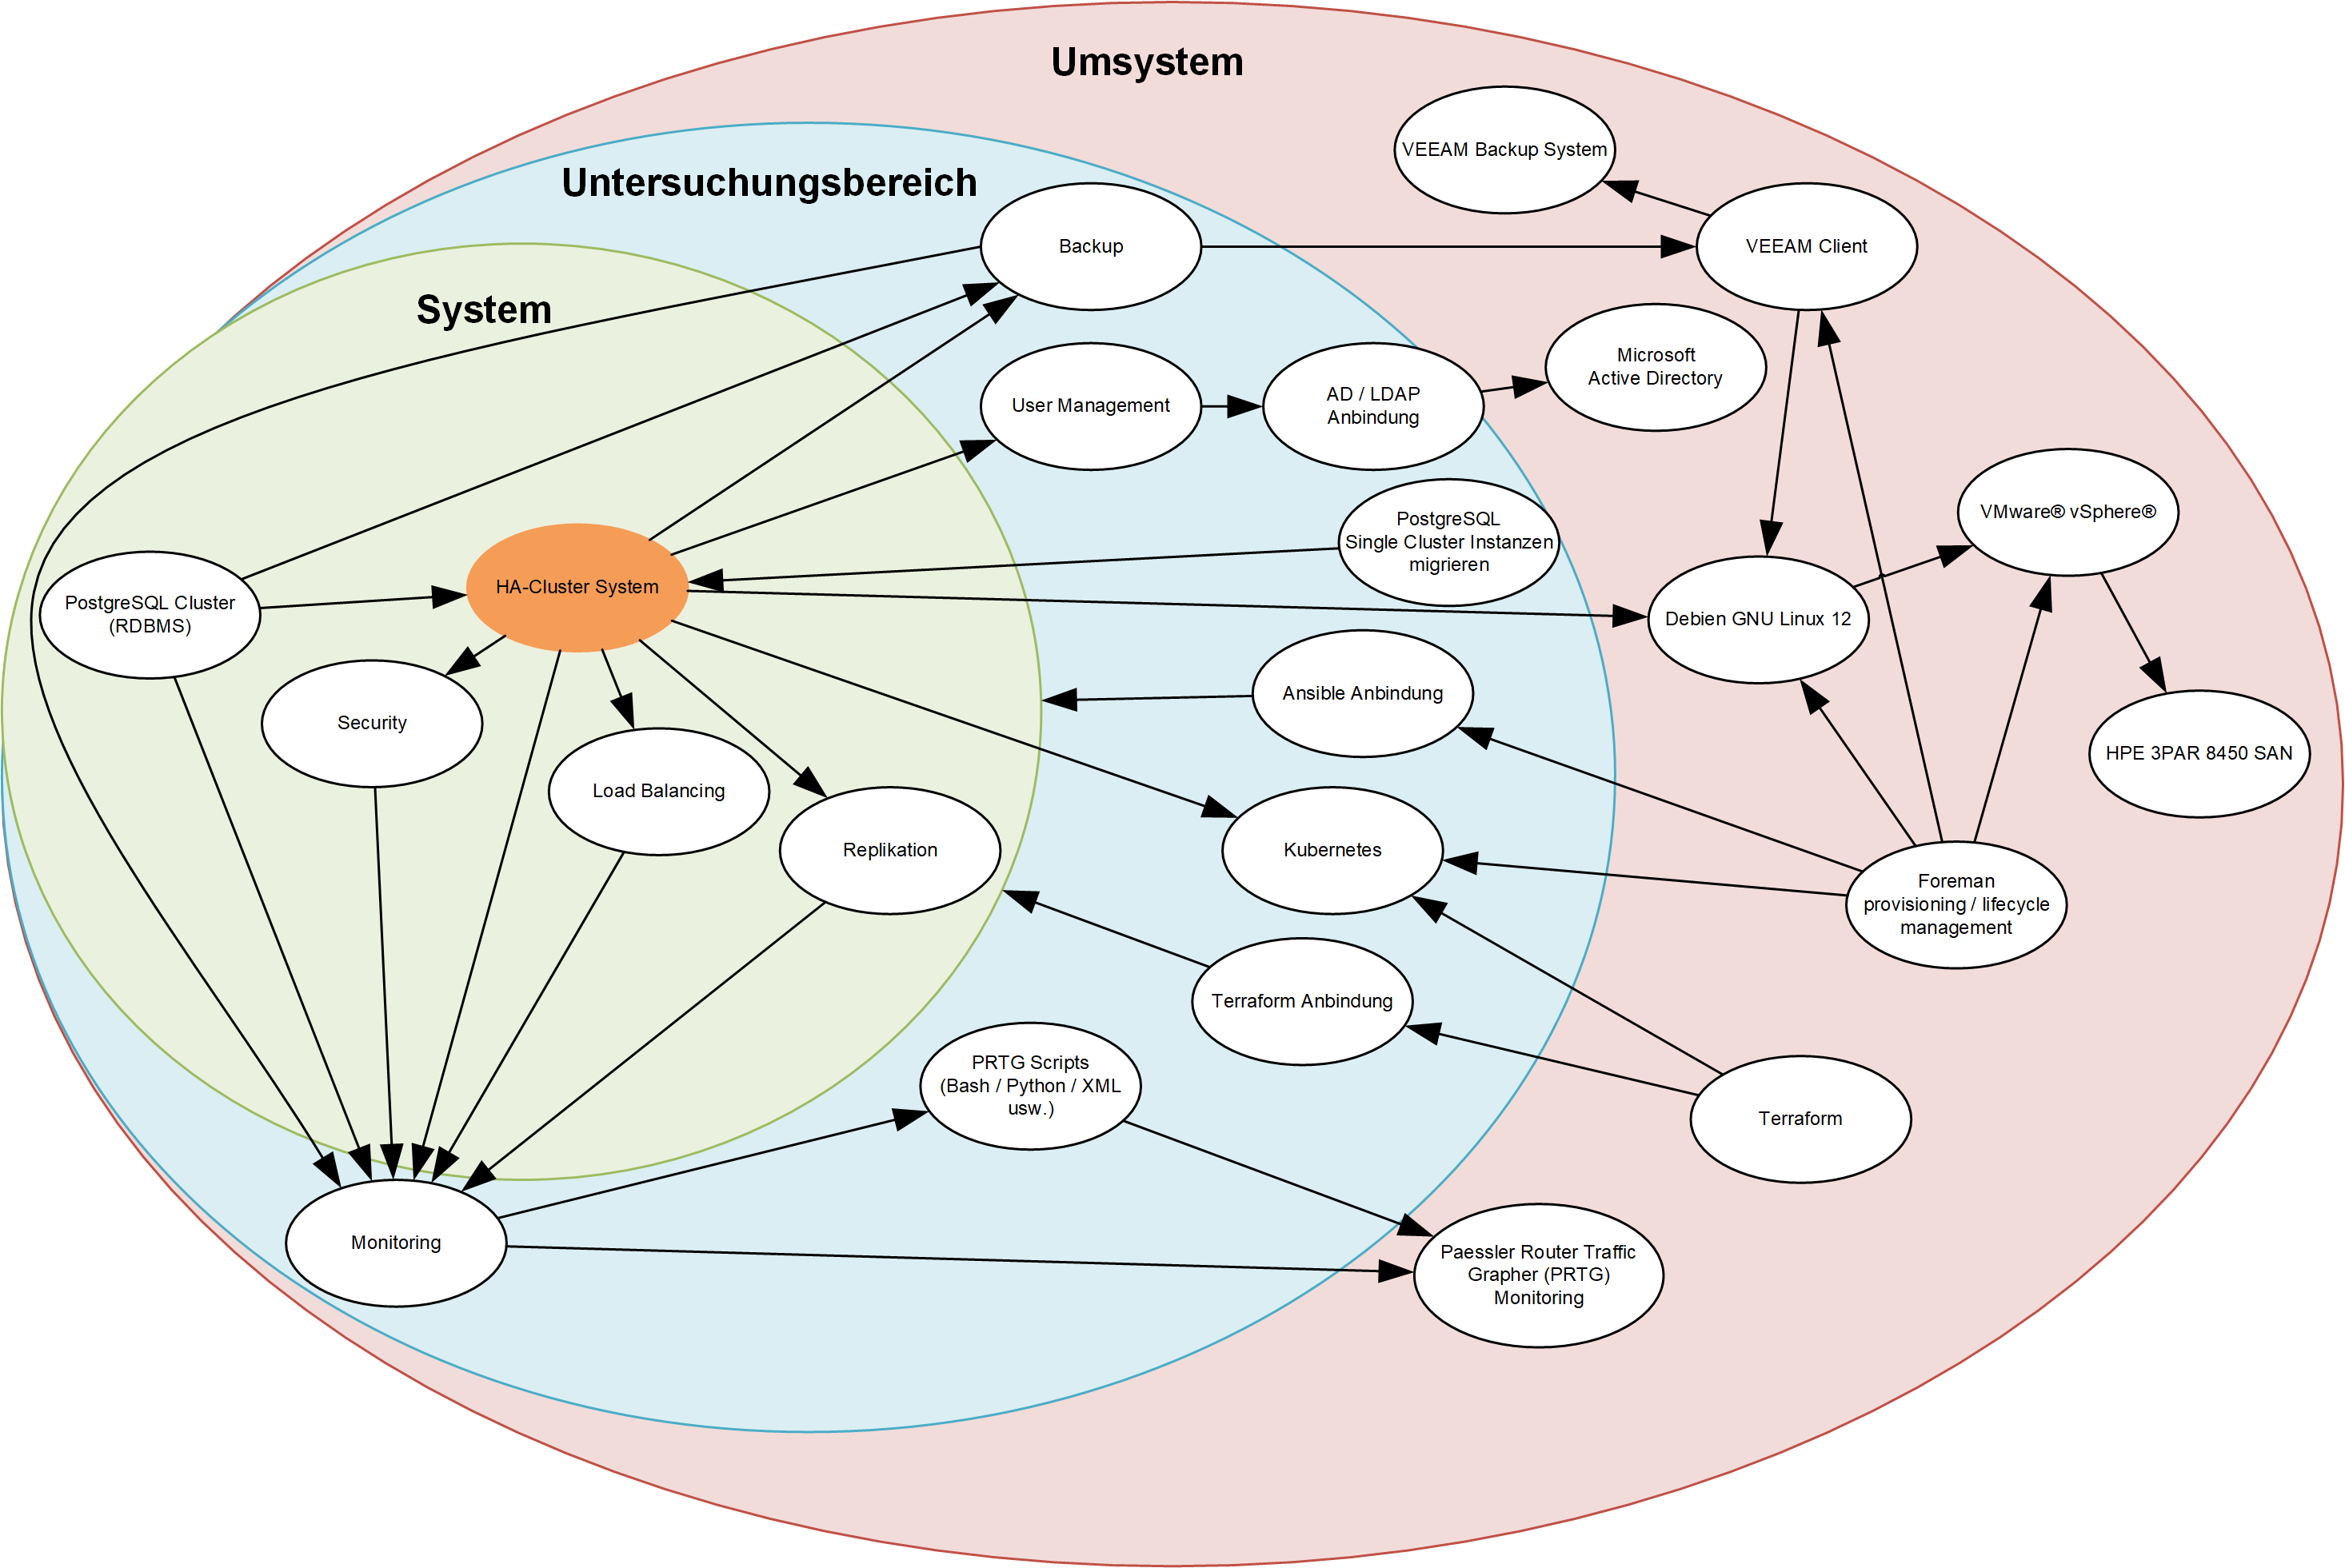
\includegraphics[width=1\linewidth]{source/introduction/delimitations/systemabgrenzungen}
        \caption{Systemabgrenzung}
        \label{fig:systemabgrenzungen}
    \end{figure}
%\end{landscape}
\clearpage
\KOMAoptions{paper=A4,paper=portrait,pagesize}
\recalctypearea


    \begin{table}[H]

\resizebox{\columnwidth}{!}{%

\begin{tabular}{rllllll}
\toprule
Nr. & Objekt & Abhängigkeit & Beschreibung & Status & Risiko & Impact \\
\midrule
1 & Foreman & \begin{tabular}[c]{@{}l@{}}VMs\end{tabular} & \begin{tabular}[c]{@{}l@{}}Das Lifecycle Management und\\Provisioning System muss zur Verfügung stehen\\um in der Evaluationsphase Develop-VMs und in der\\Installationsphase Test-VMs erstellen zu können.\end{tabular} & \begin{tabular}[c]{@{}l@{}}Im Moment ist Foreman in einer\\Proof of Concept Phase.\end{tabular} & \begin{tabular}[c]{@{}l@{}}Das Risiko besteht.\\dass Foreman nicht betriebsbereit ist\end{tabular} & \begin{tabular}[c]{@{}l@{}}VMs müssen von Hand aufgesetzt werden.\\Entsprechend wird sehr viel mehr Zeit in der\\Evaluations- und Installationsphase benötigt.\end{tabular} \\
2 & Storage & \begin{tabular}[c]{@{}l@{}}Speicher für VMs / Daten\end{tabular} & \begin{tabular}[c]{@{}l@{}}Es müssen genügend Kapazitäten auf dem Storage vorhanden sein,\\um die VMs und Datenbanken in Betrieb zu nehmen\end{tabular} & \begin{tabular}[c]{@{}l@{}}Storage wurde bereits erweitert,\\neue Disks für den SAN Storage wurden bestellt.\end{tabular} & \begin{tabular}[c]{@{}l@{}}Auf dem SAN ist keine Kapazität mehr vorhanden\end{tabular} & \begin{tabular}[c]{@{}l@{}}Es können keine VMs oder\\Datenbanken erstellt werden\end{tabular} \\
3 & Log Management / SIEM System & \begin{tabular}[c]{@{}l@{}}Sichern der Logfiles für Log Rotation\end{tabular} & \begin{tabular}[c]{@{}l@{}}Ein Log Management System / SIEM muss vorhanden sein,\\um Logs langfristig sichern zu können.\end{tabular} & \begin{tabular}[c]{@{}l@{}}Log Management und das SIAM werden abgelöst.\\Die Ausschreibung ist erfolgt\end{tabular} & \begin{tabular}[c]{@{}l@{}}Die neue Log Management Plattform\\ist noch nicht betriebsbereit\end{tabular} & \begin{tabular}[c]{@{}l@{}}Log Retention muss stark erhöht werden.\\Dies wird mehr Storage in Anspruch nehmen.\end{tabular} \\
4 & HP-UX Ablöseprojekt & \begin{tabular}[c]{@{}l@{}}Ressourcen\end{tabular} & \begin{tabular}[c]{@{}l@{}}Das Projekt zur Ablösung der HP-UX Plattform\\für die Oracle Datenbanken geht in die Konzeptions-\\und Umsetzungsphase.\end{tabular} & \begin{tabular}[c]{@{}l@{}}Umsetzungsphase.\end{tabular} & \begin{tabular}[c]{@{}l@{}}Als Oracle DBA bin ich stark in das Projekt eingebunden.\\Es besteht dass Risiko eines Ressourcenengpasses\end{tabular} & \begin{tabular}[c]{@{}l@{}}Projekt kann nicht Zeitgemäss abgeschlossen werden\end{tabular} \\
5 & GitLab & \begin{tabular}[c]{@{}l@{}}Sicherung\end{tabular} & \begin{tabular}[c]{@{}l@{}}Sicherung von Konfigurationen, Scripts usw.\end{tabular} & \begin{tabular}[c]{@{}l@{}}GitLab ist Implementiert und Betriebsbereit.\end{tabular} & \begin{tabular}[c]{@{}l@{}}GitLab steht nicht mehr zur Verfügung\end{tabular} & \begin{tabular}[c]{@{}l@{}}Keine Versionierung und Teils\\Sicherungen mehr von Konfigurationsfiles, Scripts usw.\end{tabular} \\
6 & PKI & \begin{tabular}[c]{@{}l@{}}Key Management\end{tabular} & \begin{tabular}[c]{@{}l@{}}Es braucht einen PKI um Keys und Zertifikate handeln zu können\end{tabular} & \begin{tabular}[c]{@{}l@{}}Bestehender PKI wird abgelöst.\\Ablösungsprojekt in der Initialisierungsphase.\\Bestehender PKI nicht für Zertifikate im Einsatz\end{tabular} & \begin{tabular}[c]{@{}l@{}}Es steht kein moderner PKI im Einsatz.\end{tabular} & \begin{tabular}[c]{@{}l@{}}Zertifikate können aus Zeitgründen nicht in der Evaluationsphase eingesetzt werden.\\Für die Testphase müssen Zertifikate manuell ausgestellt werden.\end{tabular} \\
\bottomrule
\end{tabular}
}
\caption{Abhängigkeiten} \label{dependencis}
\end{table}

%    %! Author = ibw
%! Date = 09.11.23

% Preamble

%Zusätzlich wurde eine \Gls{SWOT}-Analyse für das Projekt erstellt, um weitere Risiken und Gefahren für das Projekt aufzudecken.
%Dabei bezieht sich die Externe Betrachtung auf die Umsysteme und die ICT des KSGR und die Interne Betrachtung auf mich und das Team um mich herum.
%\begin{figure}[H]
%    \centering
%    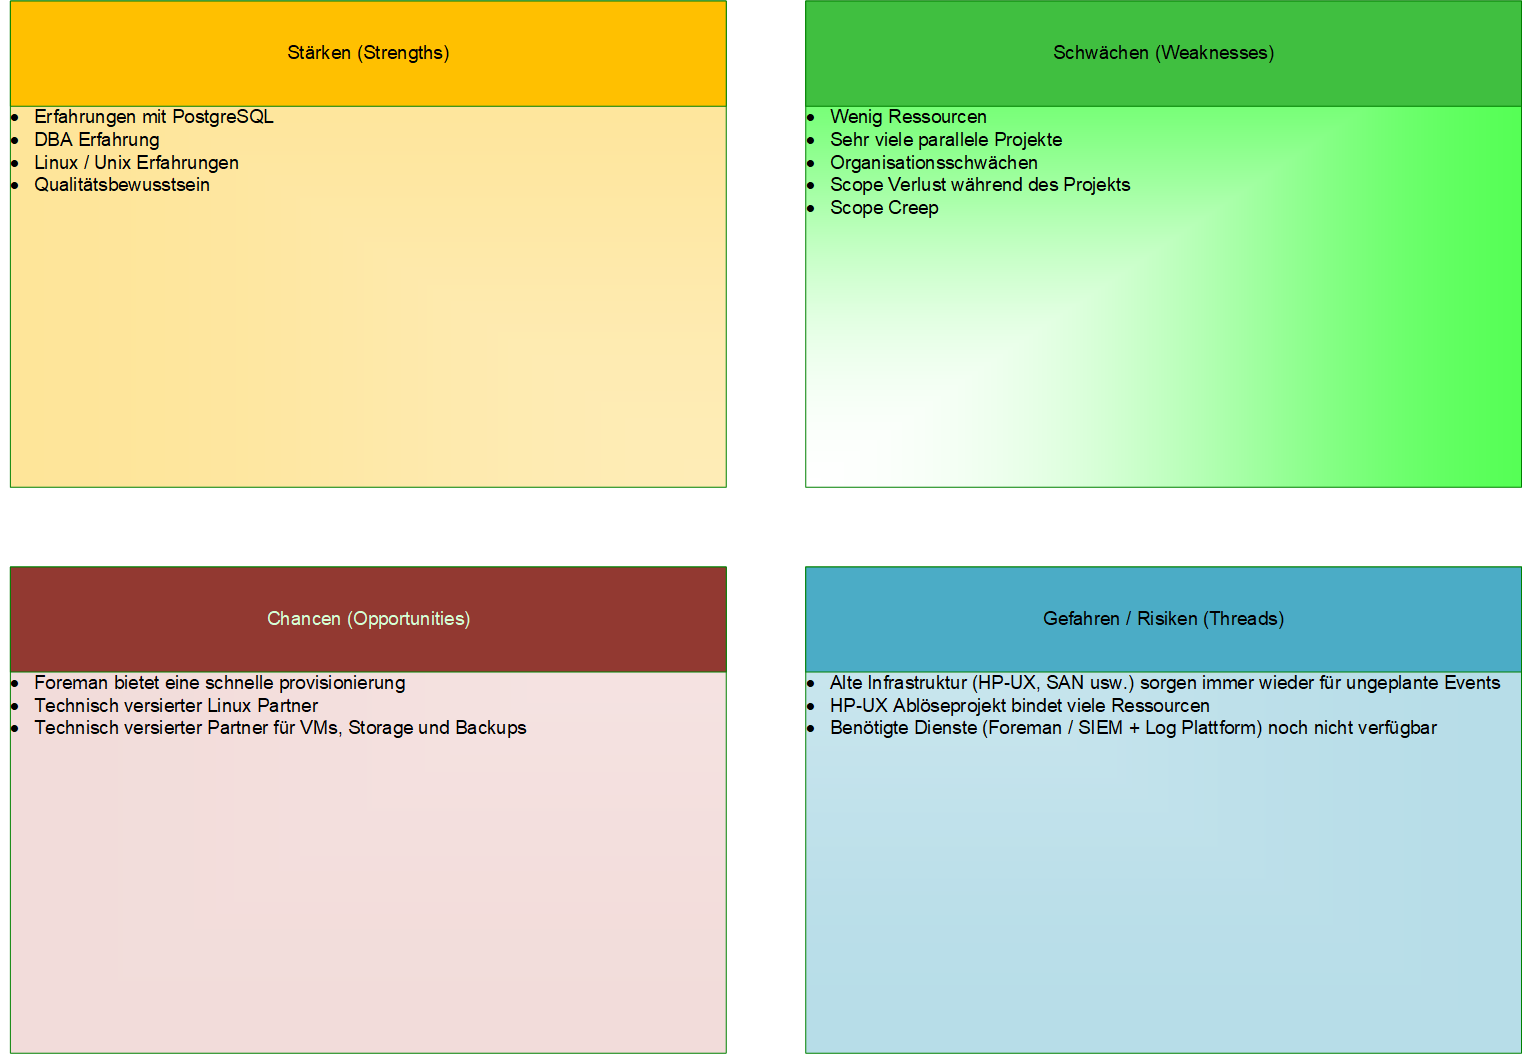
\includegraphics[width=1\linewidth]{source/introduction/riskmanagement/swot_projekt}
%    \caption{SWOT-Analyse Projekt}
%    \label{fig:swot-analysis-project}
%\end{figure}
%\begin{landscape}
%\storeareas\noraml

%\clearpage
%%\KOMAoptions{paper=A3,paper=landscape,pagesize}
%\KOMAoptions{paper=A3,paper=landscape,pagesize,DIV=20}
%\recalctypearea

\begin{flushleft}
\clearpage
%\KOMAoptions{paper=A3,paper=landscape,pagesize}
\KOMAoptions{paper=A3,paper=landscape,pagesize,DIV=20}
\recalctypearea
%\KOMAoptions{paper=A3,paper=landscape,DIV=20}
%%\storeareas\landscapevaluesbig
    \section{Risikomanagement}
    Aus den Abhängigkeiten heraus wurden folgende Risiken identifiziert:
%\end{flushleft}
\begin{table}[H]
\resizebox{\columnwidth}{!}{%
\begin{tabular}{llllllllll}
\hline
\multicolumn{2}{l}{}                                                                                           &                                                                                                                                                                                                                                                    &                                                                                                                                                                                                                                                                                             & \multicolumn{2}{l}{}                                  & \multicolumn{4}{l}{Behandlung}                                                                                                                                                                             \\ \cline{7-10}
\multicolumn{2}{l}{\multirow{-2}{*}{Identifikation}}                                                           & \multirow{-2}{*}{}                                                                                                                                                                                                                                 & \multirow{-2}{*}{}                                                                                                                                                                                                                                                                          & \multicolumn{2}{l}{\multirow{-2}{*}{Abschätzung}}     &                                         & \multicolumn{2}{l}{Zielwert} &                                                                                                                                   \\ \cline{1-6} \cline{8-9}
ID & Risiko                                                                                                    & Beschreibung / Ursache                                                                                                                                                                                                                             & Auswirkung                                                                                                                                                                                                                                                                                  & WS                        & SM                        & \multirow{-2}{*}{Massnahmen ergreifen?} & WS            & SM           & \multirow{-2}{*}{Massnahme}                                                                                                       \\ \hline
1  & Fehlende Ressourcen                                                                                       & Viele parallele Projekte, Aufträge und der Tagesbetrieb                                                                                                                                                                                            & Ressourcen während der Diplomarbeit sind knapp bemessen                                                                                                                                                                                                                                     & \cellcolor[HTML]{F8FF00}3 & \cellcolor[HTML]{F8FF00}4 & Ja                                      & 2             & 2            & \begin{tabular}[c]{@{}l@{}}Organisation und\\ Selbstmanagement\end{tabular}                                                       \\
2  & \Gls{HP-UX} Ablöseprojekt                                                                                       & \begin{tabular}[c]{@{}l@{}}Das Projekt ist sehr Umfangreich\\ und ist in die Konzeptions- und Umsetzungsphase gestartet\end{tabular}                                                                                                               & \begin{tabular}[c]{@{}l@{}}Das Projekt wird parallel zur Diplomarbeit\\ sehr viele Ressourcen und Aufmerksamkeit binden\end{tabular}                                                                                                                                                        & \cellcolor[HTML]{F8FF00}4 & \cellcolor[HTML]{F8FF00}4 & Ja                                      & 3             & 3            & Ressourcen reservieren                                                                                                            \\
3  & \begin{tabular}[c]{@{}l@{}}Alte Infrastruktur kann\\ ungeplant sämtliche Ressourcen binden\end{tabular}   & \begin{tabular}[c]{@{}l@{}}\Gls{HP-UX} Plattform, DELL NetWorker / Data Domain Umgebung\\ und HPE 3PAR \Gls{SAN} Storage Umgebung sind über dem Lifecycle\\ und haben in den vergangenen Monaten immer wieder kritische Ausfälle erlebt\end{tabular}           & \begin{tabular}[c]{@{}l@{}}Bei einem Event, ausgelöst durch das Alter der \Gls{HP-UX} Plattform,\\ der DELL NetWorker / Data Domain Umgebung oder dem SAN Storage,\\ kann der ganze Betrieb zum erliegen kommen und entsprechend\\ viele Ressourcen aufgrund der kritikalität binden\end{tabular} & \cellcolor[HTML]{F8FF00}4 & \cellcolor[HTML]{F8FF00}4 & Ja                                      & 3             & 3            & \begin{tabular}[c]{@{}l@{}}Monitoring vorgängig ausbauen\\ und Massnahmen definieren\end{tabular}                                 \\
4  & \begin{tabular}[c]{@{}l@{}}Schwächen beim\\ Selbstmanagement und\\ in der Selbstorganisation\end{tabular} & Selbstmanagement und Organisation ist nicht meine Stärke                                                                                                                                                                                           & \begin{tabular}[c]{@{}l@{}}Das Projekt verzettelt sich, Zeit geht verloren.\\ Auch eine folge könnte der Scope Verlust sein\end{tabular}                                                                                                                                                    & \cellcolor[HTML]{F8FF00}3 & \cellcolor[HTML]{F8FF00}3 & Ja                                      & 2             & 2            & \begin{tabular}[c]{@{}l@{}}Werkzeuge im Vorfeld\\ definieren und bereitstellen\end{tabular}                                       \\
5  & Scope verlust während des Projekts                                                                        & Der Scope kann während des Projekts verloren gehen                                                                                                                                                                                                 & Verzettelung und Zeitverlust bis hin zu scheitern                                                                                                                                                                                                                                           & \cellcolor[HTML]{F8FF00}3 & \cellcolor[HTML]{F8FF00}4 & Ja                                      & 2             & 3            & Ziele klar definieren                                                                                                             \\
6  & Scope Creep                                                                                               & \begin{tabular}[c]{@{}l@{}}Der Umfang kann stark steigen wenn Ziele\\ nicht genau genug definiert wurden\end{tabular}                                                                                                                              & Zeitverlust bis hin zu scheitern des Projekts                                                                                                                                                                                                                                               & \cellcolor[HTML]{F8FF00}3 & \cellcolor[HTML]{F8FF00}4 & Ja                                      & 3             & 3            & Ziele SMART definieren                                                                                                            \\
7  & SIEM / Log Plattform nicht betriebsbereit                                                                 & \begin{tabular}[c]{@{}l@{}}Die öffentliche Ausschreibung für die neue   / Log\\ Plattform wurde erst am 23.10.2023 veröffentlicht.\\ Bis zur Implementation kann noch Zeit vergehen.\end{tabular}                                              & \begin{tabular}[c]{@{}l@{}}Logs müssen länger auf dem System selber vorgehalten werden.\\ Zudem müssen ggf. eigene Massnahmen zum\\ Auslesen von Logs getroffen werden\end{tabular}                                                                                                         & \cellcolor[HTML]{F8FF00}4 & 1                         & Nein                                    &               &              &                                                                                                                                   \\
8  & \Gls{Foreman} nicht betriebsbereit                                                                              & \begin{tabular}[c]{@{}l@{}}Die \Gls{Foreman} Provisioning- und Lifecycle Plattform\\ befindet sich aktuell erst in der Proof of Concept Phase.\\ Dadurch besteht das Risiko, dass sie nicht\\ betriebsbereit zum Start der Diplomarbeit ist\end{tabular} & \begin{tabular}[c]{@{}l@{}}Ms müssen von Hand provisioniert werden.\\ Dies bedeutet einen massiven Mehraufwand und verzögert\\ ggf. die Evaluationsphase und mit sicherheit die Installationsphase\end{tabular}                                                                             & 3                         & \cellcolor[HTML]{F8FF00}5 & Ja                                      & 3             & 4            & \begin{tabular}[c]{@{}l@{}}Massnahmen ergreifen um die manuelle\\ Installation so effizient wie möglich zu gestalten.\end{tabular} \\ \hline
\end{tabular}%
}
\caption{Risiko-Matrix der Diplomarbeit}
\label{tab:riskmatrix-projekt}
\end{table}
%\end{landscape}
    \clearpage
    \KOMAoptions{paper=A4,paper=portrait,pagesize}
    \recalctypearea
\end{flushleft}
%\end{landscape}
%\begin{flushleft}
%Daraus ergibt sich folgende Risikomatrix
%\end{flushleft}
%\begin{figure}[H]
%    \centering
%    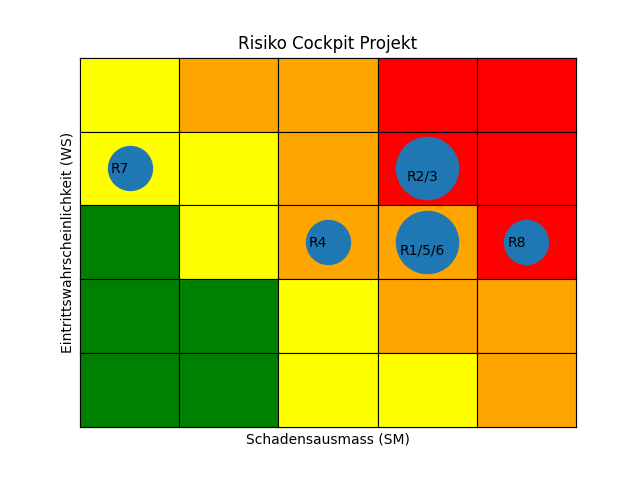
\includegraphics[width=0.75\linewidth]{source/riskmatrix/riskmatrix-project}
%    \caption{Projektrisiken}
%    \label{fig:riskmatrix-project}
%\end{figure}
%\begin{flushleft}
%Mit den entsprechenden Massnahmen können die Risiken gesenkt werden:
%\end{flushleft}
%\begin{figure}[H]
%    \centering
%    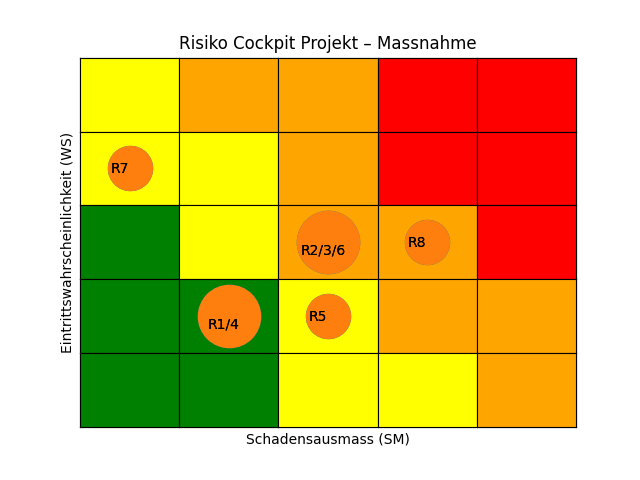
\includegraphics[width=0.75\linewidth]{source/riskmatrix/Riskmatrix-project-massnahmen}
%    \caption{Projektrisiken mit Massnahmen}
%    \label{fig:riskmatrix-project-massnahmen}
%\end{figure}

%\clearpage
%\KOMAoptions{paper=A4,paper=portrait,pagesize}
%\recalctypearea
\begin{flushleft}
%    \noraml
%    \KOMAoptions{paper=A4,paper=portrait, pagesize}
%    \clearpage
    \clearpage
    \KOMAoptions{paper=A4,paper=portrait,pagesize}
    \recalctypearea
    Daraus ergeben sich, mit den Massnahmen, folgende Risikomatrizen:
    \begin{figure}[H]
        \centering
        \subfloat{{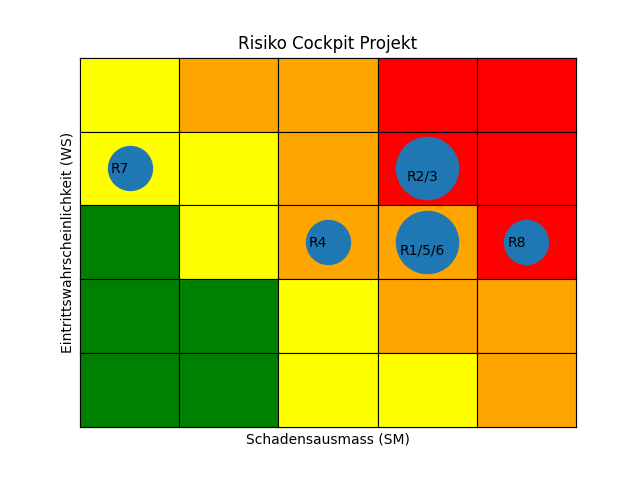
\includegraphics[width=0.47\linewidth]{source/riskmatrix/riskmatrix-project} }}%
        \qquad
        \subfloat{{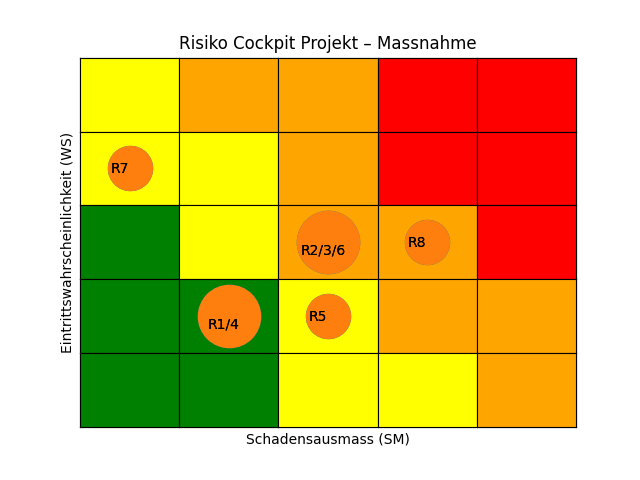
\includegraphics[width=0.47\linewidth]{source/riskmatrix/Riskmatrix-project-massnahmen} }}%
        \caption{Risikomanagement Projekt}
        \label{fig:riskmanagement_projekct}
    \end{figure}
\end{flushleft}

%    %! Author = gramic
%! Date = 21.03.24

% Preamble
%    \KOMAoptions{paper=A3,paper=landscape,DIV=20}
%\storeareas\landscapevaluesbig
%    \begin{landscape}
    \clearpage
    \KOMAoptions{paper=A3,paper=landscape,pagesize,DIV=20}
    \recalctypearea
\begin{flushleft}
    \subsection{Riskcontrolling}
    \subsubsection{Neu erfasste Risiken}
    \begin{table}[H]

\resizebox{\columnwidth}{!}{%

\begin{tabular}{rllllrrlrrl}
\toprule
ID & Definiert / Erkannt & Risiko & Beschreibung / Ursache & Auswirkung & WS & SM & Massnahmen notwendig & WS.1 & SM.1 & Massnahmen \\
\midrule
9 & \begin{tabular}[c]{@{}l@{}}19.03.2024\end{tabular} & \begin{tabular}[c]{@{}l@{}}Veeam Kasten K10\cite{P24LQGDK} nicht betriebsbereit\end{tabular} & Abhängigkeit zum KSGR k8s Projekt.\\Ohne Kubernetes kein Veeam Kasten. & \begin{tabular}[c]{@{}l@{}}Keine Kubernetes-Gerechten Sicherungen von Pods usw.\\Sicherungen Inkonsistent o.ä.\\Ohne Backup kann das Ziel des Projekts nicht erreicht werden\end{tabular} & 5 & 5 & Ja & 5 & 2 & \begin{tabular}[c]{@{}l@{}}Backup auf einem nfs-Share ablegen.\\So können Test-DBs wenigstens gesichert werden.\end{tabular} \\
\bottomrule
\end{tabular}
}
\caption{Neu Erkannte / Erfasste Risiken} \label{riskcontrolling_new_risks}
\end{table}

%    \end{landscape}
%    \begin{landscape}
        \subsubsection{Assessment 21.03.2024}
        \begin{table}[H]

\resizebox{\columnwidth}{!}{%

\begin{tabular}{rllrrllll}
\toprule
ID & Risiko & Assessment-Datum & WS & SM & Dringlichkeit & Ergriffene Massnahmen & Wirksamkeit & Begründung \\
\midrule
1 & \begin{tabular}[c]{@{}l@{}}Fehlende Ressourcen\end{tabular} & 21.03.2024 & 3 & 4 & hoch & \begin{tabular}[c]{@{}l@{}}Dokumentation ausserhalb Arbeitszeit\end{tabular} & begrenzt & \begin{tabular}[c]{@{}l@{}}Mentale Ressourcen setzen Limits.\end{tabular} \\
2 & \begin{tabular}[c]{@{}l@{}}HP-UX Ablöseprojekt\end{tabular} & 21.03.2024 & 5 & 4 & sehr hoch & \begin{tabular}[c]{@{}l@{}}Ressourcen reserviert\end{tabular} & begrenzt & \begin{tabular}[c]{@{}l@{}}ExaCC Server werden mitten während der Diplomarbeit geliefert.\\Von KSGR Seite fehlt eine Stellvertretung.\\Mithilfe notwendig.\end{tabular} \\
3 & \begin{tabular}[c]{@{}l@{}}Alte Infrastruktur kann\\ungeplant sämtliche Ressourcen binden\end{tabular} & 21.03.2024 & 4 & 4 & hoch & \begin{tabular}[c]{@{}l@{}}Externe Partner sensibilisiert\end{tabular} & wirksam & \begin{tabular}[c]{@{}l@{}}Externe Partner können meinen Teil der Aufgaben  bei Problemen abfedern.\\Allerdings nicht vollständig\end{tabular} \\
4 & \begin{tabular}[c]{@{}l@{}}Schwächen beim\\Selbstmanagement\\und in der Selbstorganisation\end{tabular} & 21.03.2024 & 3 & 3 & hoch & \begin{tabular}[c]{@{}l@{}}- Projektplanung erstellt.\\- Arbeitspakete geplant\end{tabular} & begrenzt & \begin{tabular}[c]{@{}l@{}}Nicht an alle Tasks gedacht, wie z.B. Risikocontrolling.\end{tabular} \\
5 & \begin{tabular}[c]{@{}l@{}}Scope Verlust während des Projekts\end{tabular} & 21.03.2024 & 2 & 2 & mittel & \begin{tabular}[c]{@{}l@{}}Ziele SMART definiert\end{tabular} & wirksam & \begin{tabular}[c]{@{}l@{}}Ziele sind klar definiert.\\Allerdings gibt es zwangsweise gewisse Unschärfen.\end{tabular} \\
6 & \begin{tabular}[c]{@{}l@{}}Scope Creep\end{tabular} & 21.03.2024 & 3 & 3 & hoch & \begin{tabular}[c]{@{}l@{}}Ziele SMART definiert\end{tabular} & gebrenzt & \begin{tabular}[c]{@{}l@{}}Sehr viele mögliche Lösungen am Markt.\end{tabular} \\
7 & \begin{tabular}[c]{@{}l@{}}SIEM / Log Plattform\\nicht betriebsbereit\end{tabular} & 21.03.2024 & 5 & 1 & sehr hoch & \begin{tabular}[c]{@{}l@{}}keine\end{tabular} &  & \begin{tabular}[c]{@{}l@{}}SIEM wird nicht rechtzeitig stehen.\\Das Schadensmass ist aber zu gering,\\damit Massnahmen ergriffen werden müssten.\end{tabular} \\
8 & \begin{tabular}[c]{@{}l@{}}Foreman nicht betriebsbereit\end{tabular} & 21.03.2024 & 1 & 1 & erledigt & \begin{tabular}[c]{@{}l@{}}keine\end{tabular} &  & \begin{tabular}[c]{@{}l@{}}Foreman ist in Betrieb\end{tabular} \\
9 & \begin{tabular}[c]{@{}l@{}}Veeam Kasten K10\cite{P24LQGDK} nicht betriebsbereit\end{tabular} & 21.03.2024 & 5 & 5 & sehr hoch & \begin{tabular}[c]{@{}l@{}}noch keine\end{tabular} &  & \begin{tabular}[c]{@{}l@{}}\end{tabular} \\
\bottomrule
\end{tabular}
}
\caption{Risiko-Assessment 21.03.2024} \label{risk_assessments_21_03_2024}
\end{table}

%    \end{landscape}
    \clearpage
    \KOMAoptions{paper=A4,paper=portrait,pagesize}
    \recalctypearea
\end{flushleft}
\begin{flushleft}
    \begin{figure}[H]
        \centering
        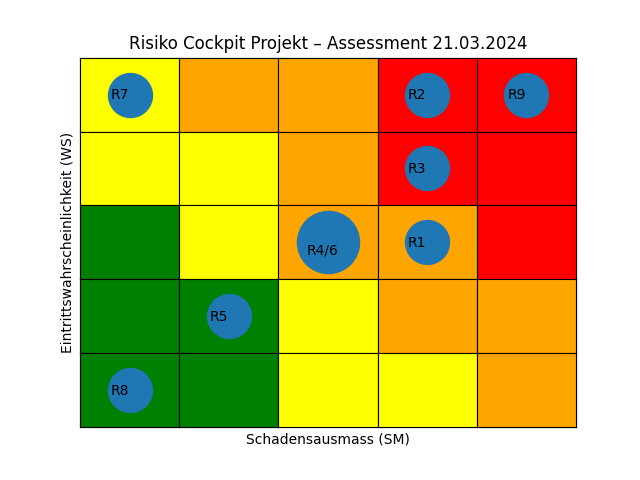
\includegraphics[width=0.75\linewidth]{source/riskmatrix/project-assessment-21-03-2024}
        \caption{Riskikomatrix - Assessment 21.03.2024}
        \label{fig:project-assessment-21-03-2024}
    \end{figure}
\end{flushleft}
%    %! Author = ibw
%! Date = 09.11.23

% Preamble
\section{Vorgehensweise und Methoden}
%    %! Author = ibw
%! Date = 09.11.23

% Preamble
%\begin{landscape}
\section{Projektmanagement}
\section{GANTT-Diagramm}
%\begin{landscape}
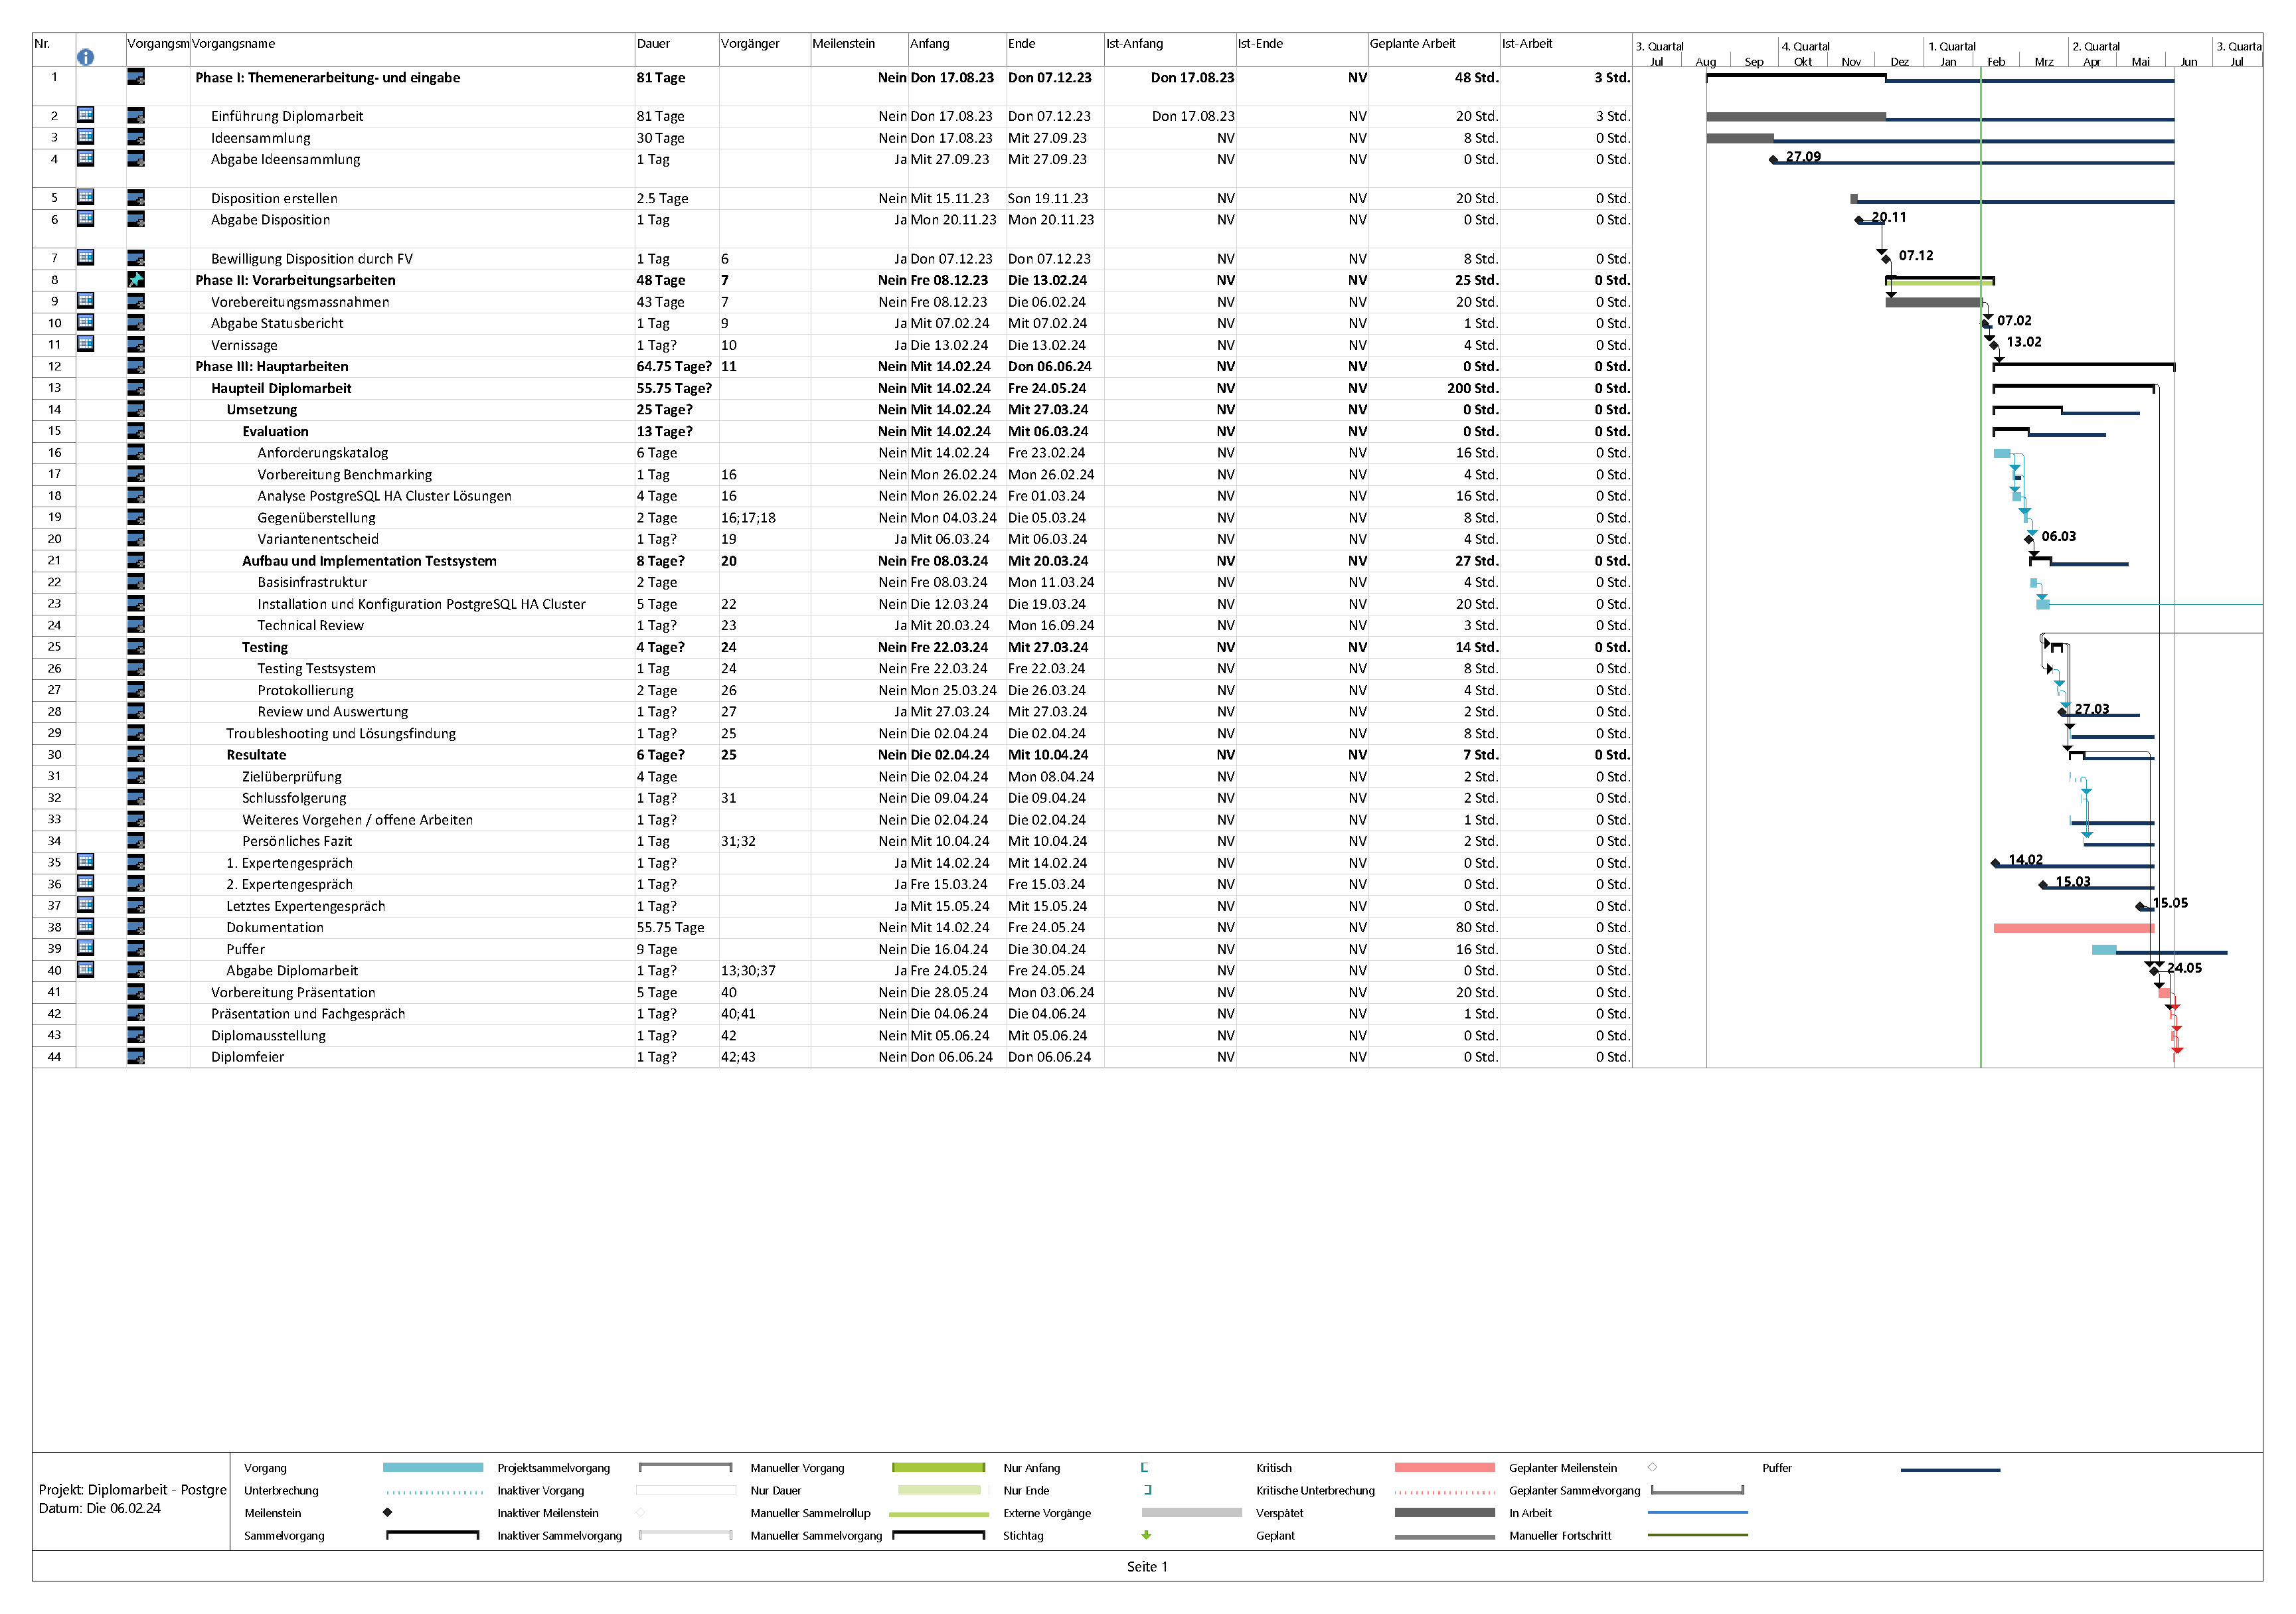
\includepdf[pages={1-},scale=1,landscape=true]{source/status_report/main/Diplomarbeit_PostgreSQL_HA_Cluster_Konzeption_und_Implementation.pdf}
%\end{landscape}
%! Author = itgramic
%! Date = 23.02.24

% Preamble
\begin{flushleft}
    \begin{landscape}
    \section{Status-Reports}
    \input{content/projectmanagement_overhead/projectmanagement/status_report/init_status}
    \input{content/projectmanagement_overhead/projectmanagement/status_report/second_status_report}
    \end{landscape}
\end{flushleft}
%\end{landscape}

%    %! Author = itgramic
%! Date = 23.02.24

% Preamble
%\begin{landscape}
    \begin{flushleft}
%        \KOMAoptions{paper=A4,paper=landscape}
%        \KOMAoptions{paper=A4,paper=landscape}
%\recalctypearea
        \storeareas\landscapevaluessmall
        \section{Expertengespräche}
        Folgende Expertengespräche fanden statt:
        \begin{table}[H]

\resizebox{\columnwidth}{!}{%

\begin{tabular}{rlllll}
\toprule
Fachgespräch & Datum & Fachexperte & Nebenexperte & Studenten & Bemerkungen \\
\midrule
1 & 14.02.2024 & Norman Süsstrunk & - & \begin{tabular}[c]{@{}l@{}}Michael Graber\\Curdin Roffler\end{tabular} & \begin{tabular}[c]{@{}l@{}}- Es wurden zwar für alle Studenten von Norman Süsstrunk Zoom-Räume bereitgestellt,\\  aus effizienzgründen nahmen Curdin Roffler und ich beide am selben Meeting teil\end{tabular} \\
2 &  & Norman Süsstrunk & - & \begin{tabular}[c]{@{}l@{}}Michael Graber\end{tabular} & \begin{tabular}[c]{@{}l@{}}\end{tabular} \\
\bottomrule
\end{tabular}
}
\caption{Fachgespräche} \label{expert_discussions_overview}
\end{table}


        Das Protokoll ist im Anhang zu finden.
    \end{flushleft}
\noraml
%\end{landscape}


\end{flushleft}
    %! Author = ibw
%! Date = 09.11.23

% Preamble
\chapter{Umsetzung}
%! Author = ibw
%! Date = 09.11.23

% Preamble
\section{Evaluation}
\subsection{Erheben und Gewichten der Anforderungen}
\subsection{Exkurs Architektur}
\subsubsection{High Availability und Replikation}
Wenn eine Datenbank HA (High Availability), also Hochverfügbar, sein soll, braucht es eine Primäre und mindestens eine Sekundäre- oder \Gls{Failover}-Datenbank.
Um Datenverlust zu vermeiden, müssen die Daten permanent von der Primären auf die sekundäre Datenbank repliziert werden, dies nennt man Replikation\cite{D9RDXENY}.
Dabei wird zwischen den folgenden beiden Replikationen unterschieden:
\\\textbf{Synchrone Replikation}\\
Wenn bei einer Synchronen Replikation eine Transaktion abgesetzt wird, wird der Commit auf der primären Seite erst gesetzt, wenn die Änderung auf der sekundären Seite oder den sekundären Seiten ebenfalls eingetragen und Committed ist.
Bis zu diesem Moment ist die Transaktion nicht als Committed.

Dies wird dann zum Problem, wenn keine Verbindung mehr zu mindesten einer sekundären Seite vorhanden ist.
Zudem wird die Synchrone Replikation bei hohen Latenzen zum Bottleneck der Datenbank.

\textbf{Asynchrone Replikation}\\
Bei der Asynchronen Replikation wird eine Transaktion erst auf der eigenen primären Seite Committed und erst dann an die sekundären Nodes gesendet.
Besonders bei hohen Latenzen bleibt die Datenbank immer perfomant, allerdings kann es je nach Latenz und genereller Auslastung zu Datenverlusten kommen, wenn es zum \Gls{Failover} kommt.
\subsubsection{Quorum}
\label{chap:Quorum}
Ein Quorum-System

Hier ein Beispiel wie sie in den Artikeln \cite{UMIGLCCI, YDS7DTYM, V4XLXN7W}
\begin{description}
    \item \textbf{Quorum}\hfill \\Die Mehrheit der Server, die einen funktionierenden Betrieb gewährleisten können, ohne eine \Gls{Split-brain}Situation zu erzeugen.
    Die Formel ist gemeinhin \(n/2 + 1\)
    \item \textbf{Throughput}\hfill \\Beschreibt, wie sich die Anzahl Nodes auf die Schreibgeschwindigkeit der Commitments auf die restlichen Nodes auswirkt.\\Die verdopplung der Server halbiert i.d.R. den Throughput.
    \item \textbf{Fehlertoleranz}\hfill \\Beschreibt, wie viele Nodes ausfallen können, damit der Cluster noch Arbeitsfähig ist.\\Wobei eine erhöhung der Nodes von 3 auf 4 die Fehlertoleranz nicht erhöht da nun eine \Gls{Split-brain}-Situation entstehen kann.
\end{description}
%\begin{landscape}
%\begin{table}[]
%\resizebox{\columnwidth}{!}{%
%\begin{tabular}{@{}llll@{}}
%\toprule
%\textbf{Anzahl Nodes} & \textbf{Quorum} & \textbf{Fehlertoleranz} & \textbf{Representative Throughput} \\ \midrule
%1                     & 1               & 0                                               & 100                                \\
%2                     & 2               & 0                                               & 85                                 \\
%3                     & 2               & 1                                               & 82                                 \\
%4                     & 3               & 1                                               & 57                                 \\
%5                     & 3               & 2                                               & 48                                 \\
%6                     & 4               & 2                                               & 41                                 \\
%7                     & 4               & 3                                               & 36                                 \\ \bottomrule
%\end{tabular}%
%}
%\caption{Quorum Beispiele}
%\label{tab:quorum-beispiele}
%\end{table}
%\end{landscape}
%\subsubsection{Split-brain}
%\label{chap:Split-brain}
\begin{table}[]
\resizebox{\columnwidth}{!}{%
\begin{tabular}{@{}llll@{}}
\toprule
\textbf{Anzahl Nodes} & \textbf{Quorum} & \textbf{Fehlertoleranz} & \textbf{Representative Throughput} \\ \midrule
1                     & 1               & 0                       & 100                                \\
2                     & 2               & 0                       & 85                                 \\
3                     & 2               & 1                       & 82                                 \\
4                     & 3               & 1                       & 57                                 \\
5                     & 3               & 2                       & 48                                 \\
6                     & 4               & 2                       & 41                                 \\
7                     & 4               & 3                       & 36                                 \\ \bottomrule
\end{tabular}%
}
\caption{Quorum Beispiele}
\label{tab:quorum-beispiele}
\end{table}
\subsubsection{CAP Theorem}
Das CAP Theorem besagt, das nur zwei der drei folgenden drei Merkmale von verteilten Systeme gewährleistet werden können\cite{EE6EQHU2}.
\\\textbf{Konsistenz - Consistency}
Die Datenbank ist Konsistent, alle Clients seher gleichzeitig die gleichen Daten unabhängig auf welchem Node das Zugegriffen wird.
Hierzu muss eine Replikation der Daten an alle Nodes stattfinden und der Commit zurückgegeben werden, also eine Synchrone Replikation stattfinden.
\\\textbf{Verfügbarkeit - Availability}
\\\textbf{Ausfalltoleranz / Partitionstoleranz - Partition tolerance}

\Gls{PostgreSQL}, \Gls{Oracle Database}oder \Gls{IBM DB2}präferieren CA, also Konsistenz und Verfügbarkeit.
\subsubsection{Skalierung}
Datenbanken müssen skalierbar sein.
Dabei wird unterschieden zwischen einer vertikalen Skalierung (scale-up) und horizontaler Skalierung (scale-out).
Bei der vertikalen Skalierung werden den DB-Servern mehr CPU-Cores und Memory sowie zum Teil Storage hinzugefügt, wobei der Storage in jedem Fall wachsen wird.
Beim horizontalen Skalieren werden weitere DB-Nodes in den Cluster eingehängt\cite{IZSGZLVT}:
\begin{figure}[H]
    \centering
    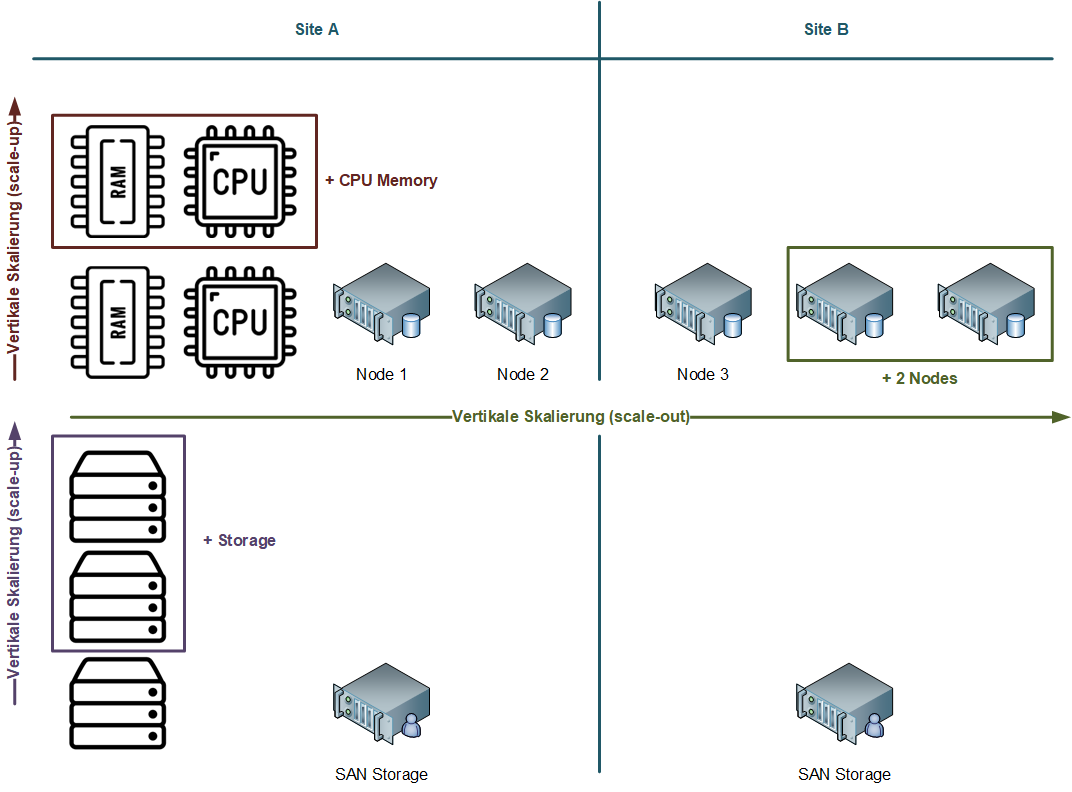
\includegraphics[width=1\linewidth]{source/implementation/evaluation/Skalierung}
    \caption{Datenbankskalierung}
    \label{fig:Datenbankskalierung}
\end{figure}

\subsection{Testziele erarbeiten}
\subsection{PostgreSQL Benchmarking}
PostgreSQL bietet ein Benchmarking-Tool,\cite{TYJFF7AB,VXNYQFTE} mit dem die DB Vermessen werden kann.
\subsection{Analyse gängiger PostgreSQL HA Cluster Lösungen}
\subsubsection{\Gls{PostgreSQL} Replikation}
PostgreSQL bietet von Haus aus Möglichkeiten, um Replikationen durchzuführen.
Dabei ist nicht jede gleich gut für jedes Szenario geeignet\cite{FZAHA89U}.

\subsubsection{KSGR Lösung}
Das Kantonsspital Graubünden hat basierend auf \gls{keepalived} wird geprüft ob die primäre Seite erreichbar und betriebsbereit ist.
Trifft dies nicht mehr zu, wird ein \Gls{Failover} durchgeführt\cite{NLF2IDBZ}.
Ist die primäre Seite wieder verfügbar, wird ein Restore auf die primäre Seite gefahren.

Es wird beim Restore immer ein komplettes Backup der sekundären Seite auf die primäre Seite übertragen.
Ursache ist, dass die normalerweise für den Datenrestore benötigten \Gls{PostgreSQL} Board mittel nur für eine relativ kurze Zeit eingesetzt werden können ehe die differenzen zwischen den beiden Seiten zu gross werden.

Bei kleinen Datenbanken wie jene für \Gls{Harbor} und \Gls{GitLab} ist die Zeit die hierfür benötigt wird, nicht relevant.
Sind die Datenbanken auf dem \Gls{PostgreSQL Cluster} jedoch grösser, kann der Restore mehrere Minuten dauern.
\subsubsection{pgpool-II}
pgpool-II ist eine Middleware die zwischen einem \Gls{PostgreSQL Cluster} und einem PostgreSQL Client gesetzt wird.
pgpoolII bietet folgende Funktionen\cite{EXVNLICT,3XWCD3KX}:
\textbf{High Availability}
pgpool-II bietet einen automatic \Gls{Failover} genannten Service an.
Dieser schwenkt auf einen Standby-Server und entfernt den Defekten Server.
Um false positive Events und Split-brains zu verhindern setzt pgpool-II auf einen eigens entwickelten \Gls{Quorum}-Algorithmus.
\\\textbf{Connection Pooling}
\\\textbf{Replikation}
\\\textbf{Load Balancing}
Ähnlich wie Oracle Active Data Guard \cite{6294443C} bietet auch pgpool-II die Möglichkeit, SELECT-Queries und Backup-Jobs auf die Secondary-Nodes umzuleiten um den Primary Node zu entlasten.
\\\textbf{Limiting Exceeding Connections}
\\\textbf{Watchdog}
\\\textbf{In Memory Query Caching}

\subsubsection{pg\_auto\_failover}
\subsubsection{Patroni}
\subsubsection{CloudNativePG}
\subsection{Installation verschiedener Lösungen}
\subsection{Gegenüberstellung der Lösungen}
\subsection{Entscheid}
%! Author = ibw
%! Date = 09.11.23

% Preamble
\begin{flushleft}
    \section{Aufbau und Implementation Testsystem}
    %! Author = gramic
%! Date = 29.04.24

% Preamble
\begin{flushleft}
    \subsection{Architektur}
    Das Testsystem wird mit Patroni umgesetzt.\\
    Dabei werden folgende Komponenten eingesetzt:\\
    \input{content/latex_tables/construction_components}
\end{flushleft}
\clearpage
\begin{flushleft}
    Entsprechend sieht das Architekturschema aus:
    \begin{figure}[H]
        \centering
        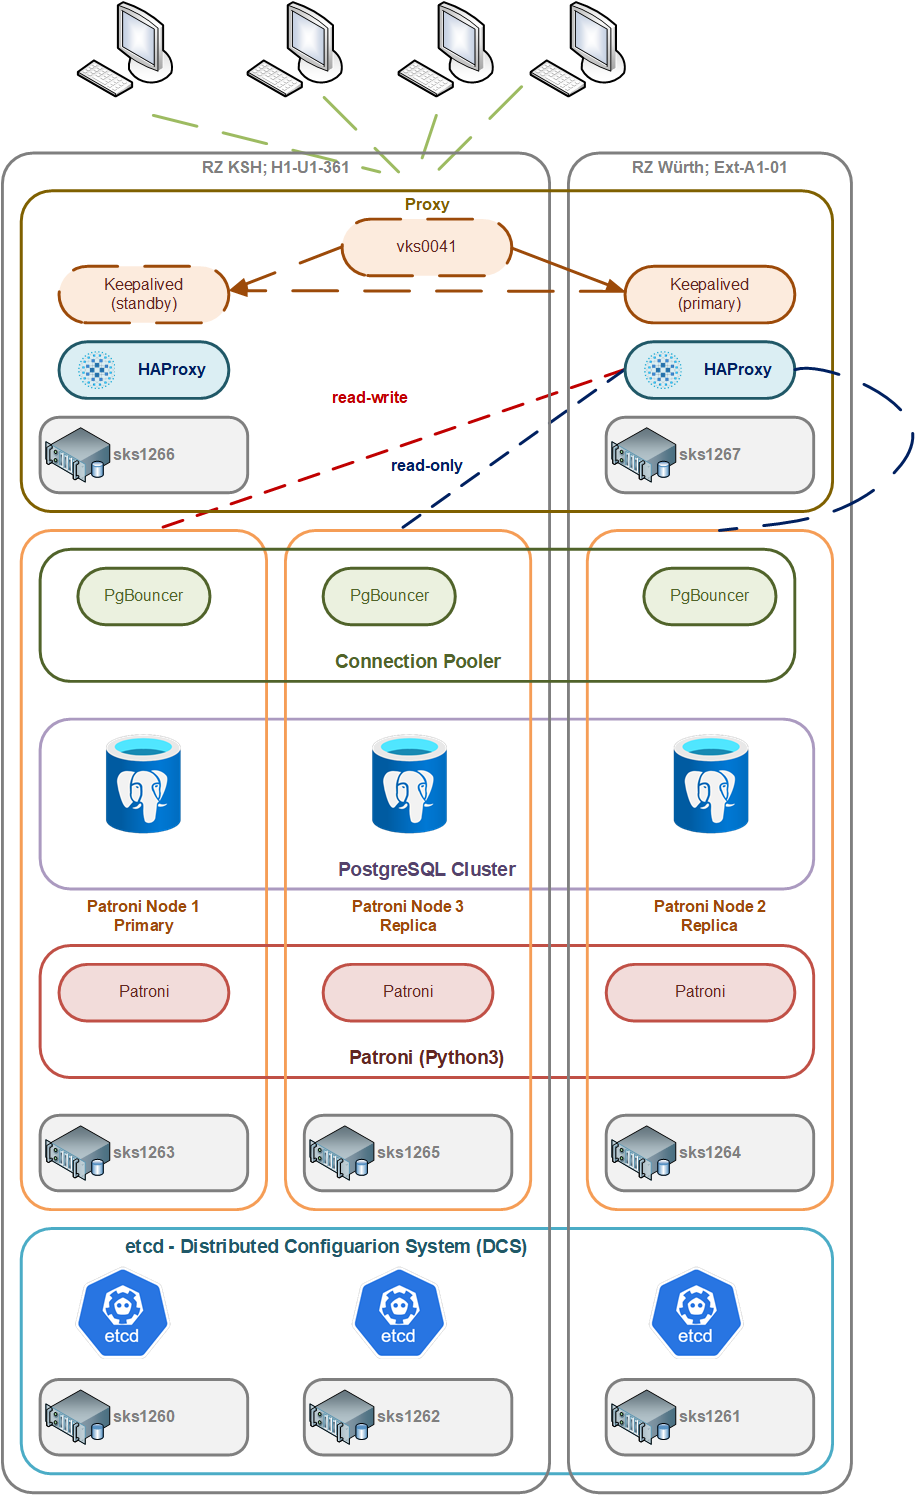
\includegraphics[width=0.7\linewidth]{source/implementation/construction_implementation/patroni-construction-architecture}
        \caption{Testsystem - Architektur}
        \label{fig:patroni-construction-architecture}
    \end{figure}
\end{flushleft}
\begin{flushleft}
    \texttt{vitabacks / postgresql\_cluster} hat eine Schwachstelle.\\
    Der \Gls{Connection Pooler} ist nicht auf dem Level des Proxy, sondern auf dem Patroni Node.\\
    Das Resultat bei einem Node Failure ist zwangsläufig, dass die Connections bei einem \Gls{Switchover} / \Gls{Failover} unterbrochen werden.\\
    Sollte die Applikation nicht fähig sein, die Connection zu halten und innerhalb eines Time-outs reconnecten zu können,\\
    kommt es zu einem Finalen Disconnect.\\
    Ohne weiteres lässt sich der \Gls{Connection Pooler} aber nicht auf den Proxy-Server verschieben, zu tief müsste in den Code eingegriffen werden.
\end{flushleft}
    \subsection{Bereitstellen der Grundinfrastruktur}
    \subsection{Installation und Konfiguration PostgreSQL HA Cluster}
    \subsection{Technical Review der Umgebung}
\end{flushleft}

%! Author = ibw
%! Date = 09.11.23

% Preamble
\section{Testing}
%! Author = gramic
%! Date = 01.05.24

% Preamble
\begin{flushleft}
    \subsubsection{Testfälle}
    \begin{description}
        \item \textbf{Basistests}\hfill \\
        \begin{enumerate}
            \item Es wird eine Verbindung auf die \texttt{postgres}- und \texttt{gramic\_test} DB\\ auf dem Host \texttt{vks0041.ksgr.ch} oder IP \texttt{10.0.22.178} auf die Ports \texttt{5000} und \texttt{5001} hergestellt
            \item Es werden Daten aus den Tabellen beide Datenbanken ausgelesen
            \item Auf die DB \texttt{gramic\_test} wird mit \texttt{pgbench} ein 5GiB-Init auf den Host \texttt{vks0041.ksgr.ch} oder IP \texttt{10.0.22.178} und Port \texttt{5000} ausgeführt
        \end{enumerate}
        \item \textbf{Failover}\hfill \\
        \begin{enumerate}[resume]
            \item Der Server des primären Nodes wird manuell rebooted.
%            \item Während dem Failover müssen Daten via SQL\\eingeführt und ausgelesen werden.
%            \item Während dem Switchover muss ein mixed \texttt{pgbench} abgesetzt werden
        \end{enumerate}
        \item \textbf{Switchover}\hfill \\
        \begin{enumerate}[resume]
            \item Mit dem \texttt{patronictl}-Command wird der Switchover gesetzt
%            \item Während dem Switchover muss ein mixed \texttt{pgbench} abgesetzt werden
        \end{enumerate}
        \item \textbf{Restore}\hfill \\
        \begin{enumerate}[resume]
            \item Der Primary Node Server muss gestoppt werden, ein mixed \texttt{pgbench} abgesetzt werden und der Server wieder gestartet werden.
            \item Mit dem \texttt{patronictl}-Command und Parameter \texttt{reinit} wird der der Node wiederhergestellt\\und abschliessend mit Hilfe von Switchover wieder als Primary gesetzt.
            \item Mit dem \texttt{patronictl}-Command und Parameter \texttt{reinit} wird der Replica-Node wiederhergestellt
            \item Vor, während und nach dem Restore müssen Tabellen mit Foreign-Key-Constraints und Daten geprüft werden.
%            \item Während dem Restore muss ein \texttt{pgbench} mixed Benchmark abgesetzt werden
        \end{enumerate}
        \item \textbf{Ansible - Deploy}\hfill \\
        \begin{enumerate}[resume]
            \item Mit \Gls{Ansible} kann der Patroni Cluster deployed werden.
        \end{enumerate}
        \item \textbf{Ansible - Maintenance}\hfill \\
        \begin{enumerate}[resume]
            \item Mit \Gls{Ansible} sollen folgende Parameter angepasst werden:
            \begin{itemize}
                \item Das \texttt{pg\_hba.conf} File.\\So dass der \Gls{HAProxy} Node \texttt{10.0.28.16} erweitert werden kann.
                \item Die Patroni REST-API soll für den jeweiligen Host von aussen ansprechbar sein.\\Entsprechend muss der Eintrag gesetzt werden
            \end{itemize}
        \end{enumerate}
        \item \textbf{Ansible - Patroni Node Extend}\hfill \\
        \begin{enumerate}[resume]
            \item Mit Hilfe eines \Gls{Ansible} Playbooks kann ein Patroni Node angehängt werden.
        \end{enumerate}
        \item \textbf{Ansible - HAproxy Node Extend}\hfill \\
        \begin{enumerate}[resume]
            \item Mit Hilfe eines \Gls{Ansible} Playbooks kann ein HAproxy Node angehängt werden.
        \end{enumerate}
    \end{description}
    \begin{warning}
        Die beiden Expansionsserver sind nicht in der \texttt{vks0041} \texttt{AD}-Gruppe und werden auch nicht via Palo Alto ans Init7 Netz gerouted.\\
        Entsprechend muss im \texttt{main.yml} der Proxy gesetzt werden.
    \end{warning}
\end{flushleft}
%! Author = gramic
%! Date = 01.05.24

% Preamble
\begin{flushleft}
    \subsection{Protokollierung}
    \input{content/latex_tables/construction_implementation_tests}
\end{flushleft}
%! Author = gramic
%! Date = 01.05.24

% Preamble
\begin{flushleft}
    \subsection{Review und Auswertung}
    \subsubsection{vitabaks/postgresql\_cluster}
    vitabaks/postgresql\_cluster ist sehr schnell und zuverlässig deployt.\\
    Das \Gls{Ansible}-Repository hat allerdings eine schwachstelle.\\
    Der \Gls{Connection Pooler} ist auf dem Level der Patroni Nodes, nicht auf dem Proxy-Level.\\
    Dadurch verliert ein Client die Verbindung, wenn der entsprechende Server nicht mehr erreichbar ist.
\end{flushleft}
\begin{flushleft}
    Auch der \Gls{HAProxy} hat eine Schwäche.\\
    Es handelt sich um einen Layer 7 Proxy, dadurch ist \Gls{HAProxy} nicht in der Lage, SQL Statements zu analysieren.\\
    Wenn also die Read-Only Statements auf die Replikas geleitet werden sollen, muss die Applikation diese auf den entsprechenden Port zugreifen.\\
    Ist die Applikation selber nicht in der Lage, die Lese- und Schreibprozesse an zwei verschiedene Ports zu leiten, geht der gesamte Load auf den Primary Node.
\end{flushleft}
\begin{flushleft}
    \subsubsection{Maintenance-Tool - Bloating Tables}
    Aufgeblähte Tabellen werden zuverlässig erkannt und die Tabelle vakuumiert.\\
    Zudem werden die Indices neu aufgebaut und somit geordnet.
    \subsubsection{Maintenance-Tool - \Gls{AUTOVACUUM}}
    Der Parameter \texttt{autovacuum\_vacuum\_scale\_factor} wird zuverlässig berechnet und abgelegt.
\end{flushleft}

%! Author = gramic
%! Date = 01.05.24

% Preamble
\begin{flushleft}
    \section{Maintenance-Tool}
    %! Author = gramic
%! Date = 10.05.24

% Preamble
\begin{flushleft}
    \subsubsection{Maintenance-Tool - Generell}
    Da das \Gls{Kubernetes} Testsystem des KSGR noch nicht freigegeben ist,\\
    wurden die Maintenance-Jobs auf der Evaluationsplattform betrieben.\\
    Dadurch ergaben sich ein paar einschränkungen.
    \begin{description}
        \item \textbf{Ressourcen}\hfill \\Ressourcen wie Python-Skripte sollten in einer Produktiven Umgebung z.B. in einem \Gls{helm} Chart abgebildet werden.\\Da die erstellung eines \gls{helm} Charts den Rahmen der Diplomarbeit sprengen würde, wurden Python-Skripte als \texttt{ConfigMap} deployt.\\In der Produktiven Umgebung ist dies tunlichst zu vermeiden!
        \item \textbf{HashiCorp Vault / Sectrets}\hfill \\Die Zugangsdaten (Username und Passwort) werden mit grosser Wahrscheinlichkeit in HashiCorp Vault\cite{ANQ2ENVU} abgebildet.\\In diesem Fall wird ein Secret deployt und das Secret als Filesystem gemountet.\\Die grösse Schwäche hierbei ist, dass die Secrets unverschlüsselt auf dem Filesystem des Pods liegen, selbst wenn mit Base64 ein Hash erzeugt wurde.\\Daher ist auch dieses Verfahren nicht für die Produktion geeignet.
        \item \textbf{Mailing}\hfill \\Mailing steht auf der Evaluationsumgebung nicht zur verfügung.
    \end{description}
\end{flushleft}
\begin{flushleft}
    Die Mainenance-Jobs sollen nach dem Microservice-Gedanken aufgebaut werden.\\
    So soll die Automatisierbarkeit erhöht und flexibilisiert werden.
\end{flushleft}
    %! Author = gramic
%! Date = 10.05.24

% Preamble
\begin{flushleft}
    \subsubsection{Maintenance-Tool - Bloated Tables / Indices}
    \paragraph{Ziel und Zweck}
    \Gls{PostgreSQL} hat mit \Gls{AUTOVACUUM} eine Funktionalität, welche Tabellen und Indizes aufräumt und bereinigt.\\
    Allerdings gelten die Parameter für den ganzen \Gls{PostgreSQL Cluster}, einzelne Tabellen werden zwangsläufig nicht optimal vakuumiert.\\
\end{flushleft}
\begin{flushleft}
    Daher war ein Ziel, dass Bloated Tables und Indices von einem Maintenance Skript erkannt und bereinigt werden.
\end{flushleft}
\begin{flushleft}
    \paragraph{Funktionsweise}
    Der Maintenance-Job soll anhand der
    Auf allen Datenbanken muss die Extension \texttt{pgstattuple} installiert werden.\\
    Die Extension sammelt und stellt Informationen über Tabellen, Indizes, Tupels usw., zur verfügung.
\end{flushleft}
\begin{flushleft}
    Mit Python werden alle Tabellen, welche bei \texttt{pgstattuple} mehr als einen konfigurationen Wert, aktuell 1.5\%, gelistet.\\
    Das SQL Statement hierzu, ist wie folgt aufgebaut:
    \lstset{style=gra_codestyle}
    \begin{lstlisting}[language=sql, caption=Maintenance-Tool - List - Maintenance-Tool - Bloated Tables / Indices,captionpos=b,label={lst:maintenannce-tool-list-bloated-tables},breaklines=true]
select
    relname as table,
    (pgstattuple(oid)).dead_tuple_percent
from pg_class
where
    relkind = 'r' and
    (pgstattuple(oid)).dead_tuple_percent > %s
order by dead_tuple_percent desc;
    \end{lstlisting}
    Anschliessend werden die entsprechenden Tabellen mittels VACUUM-Befehl manuell vakuumiert:
    \lstset{style=gra_codestyle}
    \begin{lstlisting}[language=sql, caption=Maintenance-Tool - VACUUM - Maintenance-Tool - Bloated Tables / Indices,captionpos=b,label={lst:maintenannce-tool-vacuum-bloated-tables},breaklines=true]
vacuum <table>;
    \end{lstlisting}
    \begin{warning}
        Ein \texttt{VACUUM} kann nicht in einer normalen Transaktion abgesetzt werden!\\
        Bei \texttt{psycopg2} muss der Transaktions-Isolations Level auf \texttt{ISOLATION\_LEVEL\_AUTOCOMMIT} gesetzt werden.\\
        Anders lässt sich das SQL nicht absetzen.
    \end{warning}
    Im Nachgang werden alle Indizes für die ganze Tabelle neu aufgebaut (\texttt{REINDEX}):
    \lstset{style=gra_codestyle}
    \begin{lstlisting}[language=sql, caption=Maintenance-Tool - REINDEX - Maintenance-Tool - Bloated Tables / Indices,captionpos=b,label={lst:maintenannce-tool-reindex-bloated-tables},breaklines=true]
reindex table <table>;
    \end{lstlisting}
\end{flushleft}
\begin{flushleft}
    Wichtig ist eine vorangehende Prüfung, ob ein \Gls{AUTOVACUUM}-Job am laufen ist.\\
    Trifft dies zu, darf das Skript in diesem Lauf nicht ausgeführt werden.\\
    Überprüft kann dies mit folgendem SQL werden:
    \lstset{style=gra_codestyle}
    \begin{lstlisting}[language=sql, caption=Maintenance-Tool - Check AUTOVACUUM - Maintenance-Tool - Bloated Tables / Indices,captionpos=b,label={lst:maintenannce-tool-check-autovacuum-bloated-tables},breaklines=true]
select count(*) as active from pg_stat_activity where query like 'autovacuum:%';
    \end{lstlisting}
\end{flushleft}
\begin{flushleft}
    Dem Microservice-Gedanken entsprechend, soll es pro Datenbank einen Job geben,\\
    der die Tabellen auf Bloated Tables untersucht und diese bereinigt.
\end{flushleft}
\begin{flushleft}
    Die vollständige Dokumentation ist im \hyperref[subsec:maintenance_bloated_tables]{Anhang - Maintenance-Tool - Bloated Tables} zu finden.
\end{flushleft}
    %! Author = gramic
%! Date = 10.05.24

% Preamble
\begin{flushleft}
    \subsubsection{Maintenance-Tool - AUTOVACUUM}
    \paragraph{Ziel und Zweck}
    Folgende beiden \Gls{AUTOVACUUM}-Parameter sind entscheidend für die definition, wann \Gls{AUTOVACUUM} startet:
    \begin{description}
        \item \textbf{autovacuum\_vacuum\_threshold}\hfill \\Mindestanzahl geänderter oder gelöschter Tupels die es in einer Tabelle braucht,\\damit \Gls{AUTOVACUUM} startet.\\Der Default liegt bei 50 toten Tuples.
        \item \textbf{autovacuum\_vacuum\_scale\_factor}\hfill \\Definiert, wie Prozent der Datensätze einer Datensätze geändert oder gelöscht werden müssen, bevor vakuumiert wird.
    \end{description}

    Die Grundformel, wann vakuumiert wird, sieht folgendermassen aus:\\
    \(\mathlarger{n\_dead\_tup > (pg\_class.reltuples \times autovacuum\_vacuum\_scale\_factor) + autovacuum\_vacuum\_threshold}\)
\end{flushleft}
\begin{flushleft}
    Der autovacuum\_vacuum\_scale\_factor über den gesamten \Gls{PostgreSQL Cluster} muss nun also mit der Zeit nachjustiert werden.\\
    Dazu wurde obige Formel entsprechend umgestellt, da autovacuum\_vacuum\_threshold grundsätzlich statisch bleibt:
\end{flushleft}
\begin{flushleft}
    \(\mathlarger{\mathlarger{autovacuum\_vacuum\_scale\_factor = \dfrac{(n\_dead\_tup_{max} - autovacuum\_vacuum\_threshold)}{pg\_class.reltuples}}}\)
\end{flushleft}
\begin{flushleft}
    Die Aufgabe von diesem Maintenance-Skripts ist es also nun, einmal pro Tag den autovacuum\_vacuum\_scale\_factor neu zu berechnen.\\
    Da keine Mails versendet werden können, soll bei einem sich geänderten Parameter die generierte HTML-Tabelle auf das Verzeichnis des \Gls{Kubernetes} Nodes gespeichert werden.\\
    Im Produktiven Betrieb soll die Tabelle als HTML in die Mail eingefügt werden.
    \paragraph{Funktionsweise}
    In einem ersten Schritt werden alle benötigten Parameter aus der \Gls{PostgreSQL}-Konfiguration oder den entsprechenden Katalogtabellen ausgelsen.\\
    Dies lässt sich mit einem SQL bewerkstelligen, welches wie folgt aufgebaut ist:
    \lstset{style=gra_codestyle}
    \begin{lstlisting}[language=sql, caption=Maintenance-Tool - Parameter - Maintenance-Tool - AUTOVACUUM,captionpos=b,label={lst:maintenannce-tool-parameter-maintenance-tool-autovacuum},breaklines=true]
select
    (
        select
            setting as autovacuum_vacuum_scale_factor
        from pg_settings
        where
            name = 'autovacuum_vacuum_scale_factor'
    ) as autovacuum_vacuum_scale_factor,
    (
        select
            setting as autovacuum_vacuum_threshold
        from pg_settings
        where
            name = 'autovacuum_vacuum_threshold'
    ) as autovacuum_vacuum_threshold,
    (
        select
            sum(reltuples) as reltuples
        from pg_class
    ) as reltuples,
    (
        select
            sender_host
        from pg_stat_wal_receiver
    ) as sender_host
    \end{lstlisting}
\end{flushleft}
\begin{flushleft}
    Anschliessend wird ein Python Dictionary erstellt, welches wiederum in ein pandas DataFrame umgewandelt wird.\\
    Mit der Methode \texttt{to\_html()} wird die Tabelle dann simpel auf das gemountete Host Filesystem geschrieben.\\
    Die Tabelle sieht wie folgt aus:
    \begin{figure}[H]
        \centering
        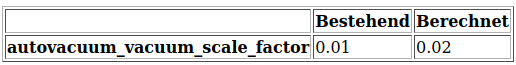
\includegraphics[width=1\linewidth]{source/implementation/construction_implementation/maintenance_tool_autovacuum/autovacuum_result_html_table}
        \caption{\Gls{AUTOVACUUM} - Berechneter autovacuum\_vacuum\_scale\_factor}
        \label{fig:autovacuum_result_html_table}
    \end{figure}
\end{flushleft}
\begin{flushleft}
    Die vollständige Dokumentation ist im \hyperref[subsec:maintenance_autovacuum]{Anhang - Maintenance-Tool - Maintenance-Tool - \Gls{AUTOVACUUM}} zu finden.
\end{flushleft}
\end{flushleft}
%! Author = gramic
%! Date = 11.05.24

% Preamble
\begin{flushleft}
    \section{Evaluationssysteme - Installation}
\end{flushleft}
%! Author = ibw
%! Date = 09.11.23

% Preamble
\begin{flushleft}
    \section{Troubleshooting und Lösungsfindung}
    Folgende Fehler sind während der Evaluation und der Installation des Testsystems aufgetreten:\\
    \begin{description}
        \item \textbf{Evaluation - Yugaware}\hfill \\Erst wurde das lizenzpflichtige Yugaware-Repository verwendet.\\Ohne Lizenzkey lässt sich Yugaware nicht installieren.\\Die Lösung bestand darin,\\auf das Open-Source YugabyteDB-Repository zu wechseln.
        \item \textbf{Evaluation - etcd für Patroni}\hfill \\Erst wurde versucht, drei etcd-Hosts auf Patroni zu installieren.\\Dies führte zu einem Hostnamenskonflikt.\\So wurde etcd auf den Standalone Server \texttt{sks9016} installiert.
        \item \textbf{Evaluation - MetalLB}\hfill \\Trotz Load Balancing mit \Gls{MetalLB} war es nicht möglich, von aussen auf YugabyteDB zuzugreifen.\\Die Kommunikation wurde nicht von \gls{rke2} von Linux an den Loead Balancer weitergegeben.\\Die Lösung bestand darin, ein sogenanntes \texttt{L2Advertisement} auf den Adress-Pool und Namespace zu setzen
        \item \textbf{Evaluation - local-path-provisioner}\hfill \\Alle Persistence Volume Claims wurden auf einen Node gesetzt.\\Solange die Volumes nicht zu gross wurden,\\war das System lauffähig.\\Bei zu grossen Volumes kam es zu einem Fehler weil die Disk in einen Overflow lief.\\Die Lösung besteht darin, im \texttt{nodePathMap} des \texttt{\gls{local-path-provisioner}} Manifests jeden Node zu spezifieren.\\Beim StorageClass-Manifest muss eine \texttt{nodeAffinity} auf die Nodes gesetzt werden.
        \item \textbf{Evaluation - StackGres Proxy für Extension}\hfill \\StackGres holt sich die PostgreSQL Extensions aus einem \Gls{GitHub} Repository.\\Da die Kommunikation über einen Proxy geht, reicht der \gls{rke2} containderd-Proxy (\texttt{CONTAINERD\_HTTPS\_PROXY} / \texttt{CONTAINERD\_HTTP\_PROXY} / \texttt{CONTAINERD\_NO\_PROXY}) nicht mehr.\\Die URL des \Gls{GitHub} Repositories muss um den Proxy erweitert werden.\\Dies löst das Problem aber nur, wenn die Zertifikate auf dem Server installiert sind.\\Andernfalls muss die Zertifikat-Prüfung umgangen werden, indem die Kommunikation mit Hilfe von \texttt{http} erzwungen wird.\\Da es sich nur um eine Evaluationsplattform handelte, kam letztere Lösung zum Einsatz.
        \item \textbf{Evaluation - Benchmarking automatisation}\hfill \\Ursprünglich war der Plan, dass die Benchmarks mit Hilfe von \texttt{pgbench} resp. \texttt{ysql\_bench} mit Hilfe von \texttt{CronJob} ausgeführt wird.\\Die beiden Benchmarking-Tools haben allerdings beide kein Passwort-Parameter.\\Auch fand sich keine gängige Lösung, das Passwort via Bypass mitgeben zu können.\\Um nicht zu viel Zeit darin zu verlieren, wurden die Benchmarks von Hand gemacht.
        \item \textbf{Testsystem - Proxy}\hfill \\Ansible konnte via Python nicht auf Externe Adressen zugreifen.\\Erst wurde manuell versucht, etcd zu installieren.\\Es gab zwei Lösungswege.
        \begin{itemize}
            \item Im \Gls{Ansible} \texttt{vars/main.yml} konnten Proxy-Settings definiert werden.\\Dann mussten trotzdem noch die apt-proxy Settings gesetzt werden.
            \item Das Netzwerkteam änderte die Zugriffspfade der Server um.\\Diese griffen nun, wenn man den Proxy ausschaltet, nicht mehr auf den Proxy zu, sondern die Palo-Firewall.\\Die dortigen Rules ermöglichen einen ausgehenden Verkehr.\\Diese Variante wird in Zukunft für \Gls{Kubernetes} Standard.
        \end{itemize}
    \end{description}
\end{flushleft}
%%! Author = gramic
%! Date = 12.05.24

% Preamble
\begin{flushleft}
    \section{Weiteres Vorgehen / offene Arbeiten}
\end{flushleft}
    %! Author = ibw
%! Date = 09.11.23

% Preamble
\chapter{Resultate}
\section{Zielüberprüfung}
\section{Schlussfolgerung}
\section{Weiteres Vorgehen / offene Arbeiten}
\section{Persönliches Fazit}
    %! Author = itgramic
%! Date = 11.10.23

% Preamble
%\printglossary
{
    \hypersetup{hidelinks}
    \listoffigures
}
\pagestyle{headings}
\thispagestyle{fancy}
{
    \hypersetup{hidelinks}
%\thispagestyle{fancy}
    \listoftables
    \thispagestyle{fancy}
}
{
    \hypersetup{hidelinks}
    \lstlistoflistings
    \thispagestyle{fancy}
}
\pagestyle{headings}
\thispagestyle{fancy}
%\begin{thebibliography}{XX}
%    \bibitem[XY]{XY} blah
%\clearpage
%\thispagestyle{fancy}
{
%    \renewcommand*\printbibliography{\thispagestyle{fancy}}
    \cleardoublepage
%    \pagestyle{headings}
%    \thispagestyle{fancy}
%    \renewcommand{\bibname}{\thispagestyle{fancy}}
%    \renewcommand{\biblatex}{\thispagestyle{fancy}}
%    \renewcommand{\bibpreamble}{\thispagestyle{fancy}}
    \renewcommand{\bibsetup}{\thispagestyle{fancy}}
%    \bibliographystyle{ieeetr}
    \printbibliography
%    \pagestyle{headings}
%    \thispagestyle{fancy}
}
{
%    \renewcommand{\glossarymark}[1]{}
%    \cleardoublepage
%    \thispagestyle{fancy}
    \renewcommand*\glossarypreamble{\thispagestyle{fancy}}
    \printnoidxglossaries
}


%\makeindex
%\printglossary[type=\acronymtype]
\begin{appendix}
%   \printglossary


        \begin{flushleft}
        \chapter*{Selbstständigkeitserklärung}
        Ich versichere, dass die vorliegende Arbeit von den Autoren selbständig und ohne Benutzung anderer als der angegebenen Hilfsmittel angefertigt wurde.
        Alle Inhalte dieser Arbeit, dazu gehören neben Texten auch Grafiken, Programmcode, etc.,
        die wörtlich oder sinngemäss aus anderen Quellen stammen, sind als solche eindeutig kenntlich gemacht und korrekt im Quellenverzeichnis gelistet.
        Dies gilt auch für einzelne Auszüge aus fremden Quellen.
        \end{flushleft}
        \begin{flushleft}
        Die Arbeit ist in gleicher oder ähnlicher Form noch nicht veröffentlicht und noch keiner Prüfungsbehörde vorgelegt worden.

        \vspace{4cm}
        \noindent
        \hrule \ \\[-0.5ex]
        Ort, Datum, Unterschrift
        \end{flushleft}
        \begin{flushleft}
        \chapter*{Haftungsausschluss}
        Der vorliegende Bericht wurde von Studierenden im Rahmen einer Diplomarbeit erarbeitet.
        Es muss an dieser Stelle darauf hingewiesen werden, dass die Arbeit nicht im Rahmen eines Auftragsverhältnisses erstellt wurde.
        Weder der Ersteller noch die ibW Höhere Fachhochschule Südostschweiz können deshalb für Aktivitäten auf der Basis dieser Diplomarbeit eine Haftung übernehmen.
        \end{flushleft}

    \renewcommand{\thesection}{\Roman{section}}
    \renewcommand{\thesubsection}{\thesection.\Roman{subsection}}
    \renewcommand{\thesubsubsection}{\thesubsection.\Roman{subsubsection}}
    \renewcommand{\theparagraph}{\thesubsubsection.\Roman{paragraph}}
    \renewcommand{\thesubparagraph}{\theparagraph.\Roman{subparagraph}}

    \titleformat{\section}[block]{\filright\normalfont\normalsize\normalcolor\fontsize{11.5pt}{13.8pt}\selectfont\rmfamily\bfseries\color[HTML]{000000}}{{\fontsize{11pt}{14.400001pt}\selectfont \makebox[2.5cm][l]{\thesection}}}{0pt}{#1}[]
    \titlespacing*{\section}{0pt}{0.847cm plus 0.1694cm minus 0.0847cm}{0.212cm plus 0.0424cm minus 0.0212cm}
    \titleformat{\subsection}[block]{\filright\normalfont\normalsize\normalcolor\fontsize{10pt}{13.8pt}\selectfont\rmfamily\bfseries\color[HTML]{000000}}{{\fontsize{11pt}{14.400001pt}\selectfont \makebox[2.5cm][l]{\thesubsection}}}{0pt}{#1}[]
    \titlespacing*{\subsection}{0pt}{0.847cm plus 0.1694cm minus 0.0847cm}{0.212cm plus 0.0424cm minus 0.0212cm}
    \titleformat{\subsubsection}[block]{\filright\normalfont\normalsize\normalcolor\fontsize{10pt}{13.8pt}\selectfont\rmfamily\bfseries\color[HTML]{000000}}{{\fontsize{11pt}{14.400001pt}\selectfont \makebox[2.5cm][l]{\thesubsubsection}}}{0pt}{#1}[]
    \titlespacing*{\subsubsection}{0pt}{0.847cm plus 0.1694cm minus 0.0847cm}{0.212cm plus 0.0424cm minus 0.0212cm}
%    \titleformat{\subsubsection}[block]{\filright\normalfont\normalsize\normalcolor\fontsize{10pt}{13.8pt}\selectfont\rmfamily\bfseries\color[HTML]{000000}}{{\fontsize{11pt}{14.400001pt}\selectfont \makebox[2.5cm][l]{\thesubsubsection}}}{0pt}{#1}[]
%    \titlespacing*{\subsubsection}{0pt}{0.847cm plus 0.1694cm minus 0.0847cm}{0.212cm plus 0.0424cm minus 0.0212cm}
    \titleformat{\paragraph}[block]{\filright\normalfont\normalsize\normalcolor\fontsize{10pt}{13.8pt}\selectfont\rmfamily\bfseries\color[HTML]{000000}}{{\fontsize{11pt}{14.400001pt}\selectfont \makebox[2.5cm][l]{\theparagraph}}}{0pt}{#1}[]
    \titlespacing*{\paragraph}{0pt}{0.847cm plus 0.1694cm minus 0.0847cm}{0.212cm plus 0.0424cm minus 0.0212cm}
    \titleformat{\subparagraph}[block]{\filright\normalfont\normalsize\normalcolor\fontsize{10pt}{13.8pt}\selectfont\rmfamily\bfseries\color[HTML]{000000}}{{\fontsize{11pt}{14.400001pt}\selectfont \makebox[2.5cm][l]{\thesubparagraph}}}{0pt}{#1}[]
    \titlespacing*{\subparagraph}{0pt}{0.847cm plus 0.1694cm minus 0.0847cm}{0.212cm plus 0.0424cm minus 0.0212cm}

    \captionsetup[table]{name=TABLE}
    \renewcommand{\thetable}{\Roman{table}}

    \clearpage
    \addcontentsline{toc}{chapter}{Anhang}
    \addtocontents{toc}{%
    \protect\addtokomafont{chapterentry}{Anhang\ }
%    \pagenumbering{roman}
%    \setcounter{page}{1}
    }
    \pagenumbering{roman}
    \setcounter{page}{1}
%\listofatoc
%\tableofcontents
    %! Author = itgramic
%! Date = 12.01.24

% Preamble
\section{Statusbericht}
\subsection{}
    %! Author = ibw
%! Date = 10.11.23

% Preamble
\subsection{Rapport}
%    %! Author = itgramic
%! Date = 24.01.24

% Preamble
\section{minikube}
    %! Author = itgramic
%! Date = 26.01.24

% Preamble
\section{rke2}
\subsection{Vorbereitung}
Da Package aus WAN-Repositories geladen werden, muss eine Proxy-Connection nach aussen gemacht werden können:
\lstset{style=gra_codestyle}
\begin{lstlisting}[language=bash, caption=Proxy Settings,captionpos=b,label={lst:proxy-settings},breaklines=true]
sudo nano /etc/profile.d/proxy.sh

export https_proxy=http://sproxy.sivc.first-it.ch:8080
export HTTPS_PROXY=http://sproxy.sivc.first-it.ch:8080
export http_proxy=http://sproxy.sivc.first-it.ch:8080
export HTTP_PROXY=http://sproxy.sivc.first-it.ch:8080
export no_proxy=localhost,127.0.0.0/8,::1,10.0.0.0/8,172.16.0.0/12,192.168.0.0/16
export NO_PROXY=localhost,127.0.0.0/8,::1,10.0.0.0/8,172.16.0.0/12,192.168.0.0/16

source /etc/profile.d/proxy.sh
\end{lstlisting}

\subsection{Installation}
\subsubsection{server - sks1183}
Es gibt kein apt-Package.
Daher muss zuerst das tarball-Package heruntergeladen werden.

Zuerst wird das Verzeichnis für rke2 erstellt:
\lstset{style=gra_codestyle}
\begin{lstlisting}[language=bash, caption=rke2 server - Verzeichnis erstellen,captionpos=b,label={lst:rke2-server-mkdir-rke2},breaklines=true]
mkdir -p /etc/rancher/rke2/
mkdir -p /var/lib/rancher/rke2/server/manifests/
\end{lstlisting}

\lstset{style=gra_codestyle}
\begin{lstlisting}[language=yaml, caption=rke2 server - config.yaml,captionpos=b,label={lst:rke2-server-config.yaml},breaklines=true]
# /etc/rancher/rke2/
cluster-cidr: "198.18.0.0/16"
service-cidr: "198.19.0.0/16"
cni:
  - cilium
disable:
  - rke2-canal
\end{lstlisting}

Cilium muss separat manifestiert werden:
\lstset{style=gra_codestyle}
\begin{lstlisting}[language=yaml, caption=rke2 server - cilium-config.yaml,captionpos=b,label={lst:rke2-server-cilium-config.yaml},breaklines=true]
# /var/lib/rancher/rke2/server/manifests/rke2-cilium-config.yaml
---
apiVersion: helm.cattle.io/v1
kind: HelmChartConfig
metadata:
  name: rke2-cilium
  namespace: kube-system
spec:
  valuesContent: |-
    eni:
      enabled: true
\end{lstlisting}

Das Package kann nun installiert und aktiviert werden:
\lstset{style=gra_codestyle}
\begin{lstlisting}[language=bash, caption=rke2 server installieren,captionpos=b,label={lst:install-rke2-server},breaklines=true]
curl -sfL https://get.rke2.io | INSTALL_RKE2_VERSION=v1.29.0+rke2r1 sh -
systemctl enable rke2-server.service
systemctl start rke2-server.service
\end{lstlisting}

\subsubsection{agents - sks1184 / sks1185}
Der Agent muss direkt heruntergeladen, installiert und aktiviert werden:
\lstset{style=gra_codestyle}
\begin{lstlisting}[language=bash, caption=rke2 agenten installieren,captionpos=b,label={lst:install-rke2-agent},breaklines=true]
curl -sfL https://get.rke2.io | INSTALL_RKE2_TYPE="agent" INSTALL_RKE2_VERSION=v1.29.0+rke2r1 sh -
systemctl enable rke2-agent.service
mkdir -p /etc/rancher/rke2/
\end{lstlisting}

Die Konfiguration muss nun konfiguriert werden.
Dem Agents müssen den Server und den Server Token erhalten:
\lstset{style=gra_codestyle}
\begin{lstlisting}[language=yaml, caption=rke2 agent - config.yaml,captionpos=b,label={lst:rke2-agent-config.yaml},breaklines=true]
# /etc/rancher/rke2/config.yaml
server: https://10.0.20.97:9345
token: K1042bf32f28282edad37cbac4b77ccfa1cd44a26f0ea2c19111ed664013954a326::server:7a430a28b29501b778543f0882a156b8
\end{lstlisting}

Nun muss der Dienst restartet werden
\lstset{style=gra_codestyle}
\begin{lstlisting}[language=bash, caption=-rke2 agent service restart,captionpos=b,label={lst:rke2-agent-service-restart},breaklines=true]
systemctl start rke2-agent.service
\end{lstlisting}

\subsection{Cluster Konfiguration}
\subsubsection{server}
Auch für Kubernetes und die Pots müssen die Proxy-Einstellungen gemacht werden:
\lstset{style=gra_codestyle}
\begin{lstlisting}[language=bash, caption=rke2 server proxy,captionpos=b,label={lst:rke2-server-proxy},breaklines=true]
nano /etc/default/rke2-server
HTTPS_PROXY=http://sproxy.sivc.first-it.ch:8080
HTTP_PROXY=http://sproxy.sivc.first-it.ch:8080
NO_PROXY=localhost,127.0.0.0/8,::1,10.0.0.0/8,172.16.0.0/12,192.168.0.0/16

CONTAINERD_HTTPS_PROXY=http://sproxy.sivc.first-it.ch:8080
CONTAINERD_HTTP_PROXY=http://sproxy.sivc.first-it.ch:8080
CONTAINERD_NO_PROXY=localhost,127.0.0.0/8,::1,10.0.0.0/8,172.16.0.0/12,192.168.0.0/16
\end{lstlisting}

Dieses File muss entsprechend in das Homeverzeichnis gespeichert werden:
\lstset{style=gra_codestyle}
\begin{lstlisting}[language=bash, caption=rke2 server proxy kopieren,captionpos=b,label={lst:rke2-server-proxy-copy},breaklines=true]

\end{lstlisting}

Für den Netzwerkteil muss nun Cilium installiert werden:
\lstset{style=gra_codestyle}
\begin{lstlisting}[language=bash, caption=rke2 server cilium installieren,captionpos=b,label={lst:rke2-server-cilium-install},breaklines=true]

\end{lstlisting}

Cilium muss nun aktiviert werden:
\begin{lstlisting}[language=bash, caption=rke2 server cilium aktivieren,captionpos=b,label={lst:rke2-server-cilium-apply},breaklines=true]

\end{lstlisting}

Der rke2-Server muss nun mit der entsprechenden Config gestartet werden, anschliessend muss Cilium noch in die Conig und diese mittels Service reboot aktiviert werden:
\lstset{style=gra_codestyle}
\begin{lstlisting}[language=bash, caption=rke2 server starten,captionpos=b,label={lst:rke2-server-start},breaklines=true]

\end{lstlisting}

Entsprechend muss die Firewall gesetzt werden:
\lstset{style=gra_codestyle}
\begin{lstlisting}[language=bash, caption=iptables entries server,captionpos=b,label={lst:iptables-server-entries},breaklines=true]
nano /etc/iptables/rules.v4

# Generated by iptables-save v1.8.9 (nf_tables)
*filter
:INPUT DROP [0:0]
:FORWARD ACCEPT [0:0]
:OUTPUT ACCEPT [0:0]
-A INPUT -m state --state RELATED,ESTABLISHED -j ACCEPT
-A INPUT -p udp -m udp --sport 53 -j ACCEPT
-A INPUT -p icmp -j ACCEPT
-A INPUT -i lo -j ACCEPT
-A INPUT -s 10.0.0.0/8 -p tcp -m tcp --dport 22 -j ACCEPT
-A INPUT -s 10.0.9.115/32 -p udp -m udp --dport 161 -m comment --comment "Allow SNMP for probe 10.0.9.115" -j ACCEPT
-A INPUT -s 10.0.9.76/32 -p udp -m udp --dport 161 -m comment --comment "Allow SNMP for probe 10.0.9.76" -j ACCEPT
-A INPUT -s 10.0.36.147/32 -p udp -m udp --dport 161 -m comment --comment "Allow SNMP for probe 10.0.36.147" -j ACCEPT
-A INPUT -s 10.0.9.35/32 -p udp -m udp --dport 161 -m comment --comment "Allow SNMP for probe 10.0.9.35" -j ACCEPT
-A INPUT -s 10.0.9.37/32 -p udp -m udp --dport 161 -m comment --comment "Allow SNMP for probe 10.0.9.37" -j ACCEPT
-A INPUT -s 10.0.9.74/32 -p udp -m udp --dport 161 -m comment --comment "Allow SNMP for probe 10.0.9.74" -j ACCEPT
-A INPUT -s 10.0.9.75/32 -p udp -m udp --dport 161 -m comment --comment "Allow SNMP for probe 10.0.9.75" -j ACCEPT
-A INPUT -s 10.0.9.36/32 -p udp -m udp --dport 161 -m comment --comment "Allow SNMP for probe 10.0.9.36" -j ACCEPT
-A INPUT -s 10.0.9.14/32 -p udp -m udp --dport 161 -m comment --comment "Allow SNMP for probe 10.0.9.14" -j ACCEPT
-A INPUT -s 10.0.0.0/8 -p icmp -m icmp --icmp-type 8 -j ACCEPT
-A INPUT -s 10.0.0.0/8 -p tcp -m tcp --dport 6443 -j ACCEPT
-A INPUT -s 10.0.0.0/8 -p tcp -m tcp --dport 9345 -j ACCEPT
COMMIT
# Completed

systemctl restart iptables
\end{lstlisting}

Für den Connect der Agents muss noch ein Token generiert werden:
\begin{lstlisting}[language=bash, caption=rke2 server token,captionpos=b,label={lst:rke2-server-token},breaklines=true]
\end{lstlisting}

\subsubsection{agents}

\subsubsection{local-path-provisioner}
Zuerst mussten auf den drei Servern der Storage bereitgestellt werden:
\lstset{style=gra_codestyle}
\begin{lstlisting}[language=bash, caption=local-path-storage auf Linux Bereitstellen,captionpos=b,label={lst:local-path-storage-provide},breaklines=true]
root@sks1183:~# mkdir /var/local-path-provisioner
root@sks1183:~# chmod -R 777 /var/local-path-provisioner/

root@sks1184:~# mkdir /var/local-path-provisioner
root@sks1184:~# chmod -R 777 /var/local-path-provisioner/

root@sks1185:~# mkdir /var/local-path-provisioner
root@sks1185:~# chmod -R 777 /var/local-path-provisioner/
\end{lstlisting}

Anschliessend musste rke2 entsprechend angepasst werden.
Damit Automatisch der local-path auf das Verzeichnis \texttt{/var/local-path-provisioner/} geht, muss dies in einem entsprechenden Manifest geschrieben werden:
\lstset{style=gra_codestyle}
\begin{lstlisting}[language=yaml, caption=local-path-provisioner definieren,captionpos=b,label={lst:local-path-provisioner.yaml},breaklines=true]
kind: ConfigMap
apiVersion: v1
metadata:
  name: local-path-config
  namespace: local-path-storage
data:
  config.json: |-
        {
                "nodePathMap":[
                {
                        "node":"DEFAULT_PATH_FOR_NON_LISTED_NODES",
                        "paths":["/var/local-path-provisioner"]
                }
                ]
        }
  setup: |-
        #!/bin/sh
        set -eu
        mkdir -m 0777 -p "$VOL_DIR"
  teardown: |-
        #!/bin/sh
        set -eu
        rm -rf "$VOL_DIR"
  helperPod.yaml: |-
        apiVersion: v1
        kind: Pod
        metadata:
          name: helper-pod
        spec:
          priorityClassName: system-node-critical
          tolerations:
            - key: node.kubernetes.io/disk-pressure
              operator: Exists
              effect: NoSchedule
          containers:
          - name: helper-pod
            image: busybox
\end{lstlisting}


Zuerst mussten auf den drei Servern der Storage bereitgestellt werden:
\lstset{style=gra_codestyle}
\begin{lstlisting}[language=bash, caption=local-path-storage aktualisieren,captionpos=b,label={lst:local-path-storage-apply},breaklines=true]
kubectl apply -f /home/gramic/PycharmProjects/rke2_settings/rke2/local-path-provisioner.yaml
\end{lstlisting}

\subsubsection{MetallB - Proxy / Load Balancer}
MetallB musste installiert werden:
\lstset{style=gra_codestyle}
\begin{lstlisting}[language=bash, caption=MetallB installieren,captionpos=b,label={lst:metallb-install},breaklines=true]
kubectl apply -f https://raw.githubusercontent.com/metallb/metallb/v0.14.4/config/manifests/metallb-native.yaml
\end{lstlisting}

Das Konfigurationsmanifest wurde eingespielt:
\lstset{style=gra_codestyle}
\begin{lstlisting}[language=yaml, caption=MetallB konfigurieren,captionpos=b,label={lst:metallb-config},breaklines=true]
apiVersion: metallb.io/v1beta1
kind: IPAddressPool
metadata:
  name: distributed-sql
  namespace: metallb-system
spec:
  addresses:
  - 10.0.20.106-10.0.20.106
  - 10.0.20.150-10.0.20.155
\end{lstlisting}

Das Manifest musste danach eingespielt werden:
\lstset{style=gra_codestyle}
\begin{lstlisting}[language=bash, caption=MetallB Konfiguration einspielen,captionpos=b,label={lst:metallb-apply},breaklines=true]
kubectl apply -f /home/gramic/PycharmProjects/rke2_settings/rke2/metallb-values.yaml
\end{lstlisting}


    %! Author = ibw
%! Date = 10.11.23

% Preamble
\subsection{pgpoolII}
    %! Author = gramic
%! Date = 15.03.24

% Preamble
\begin{flushleft}
    \subsubsection{yugabyteDB}
    \paragraph{Installation}
    Wähend der Installation des YugabyteDB Evaluations-Enviroment wurde festgestellt, das man zwei Varianten Installieren kann.
    YugabyteDB (Repository yugabyte) und YugabyteDB Anywhere (Repository yugawre):
    \begin{figure}[H]
        \centering
        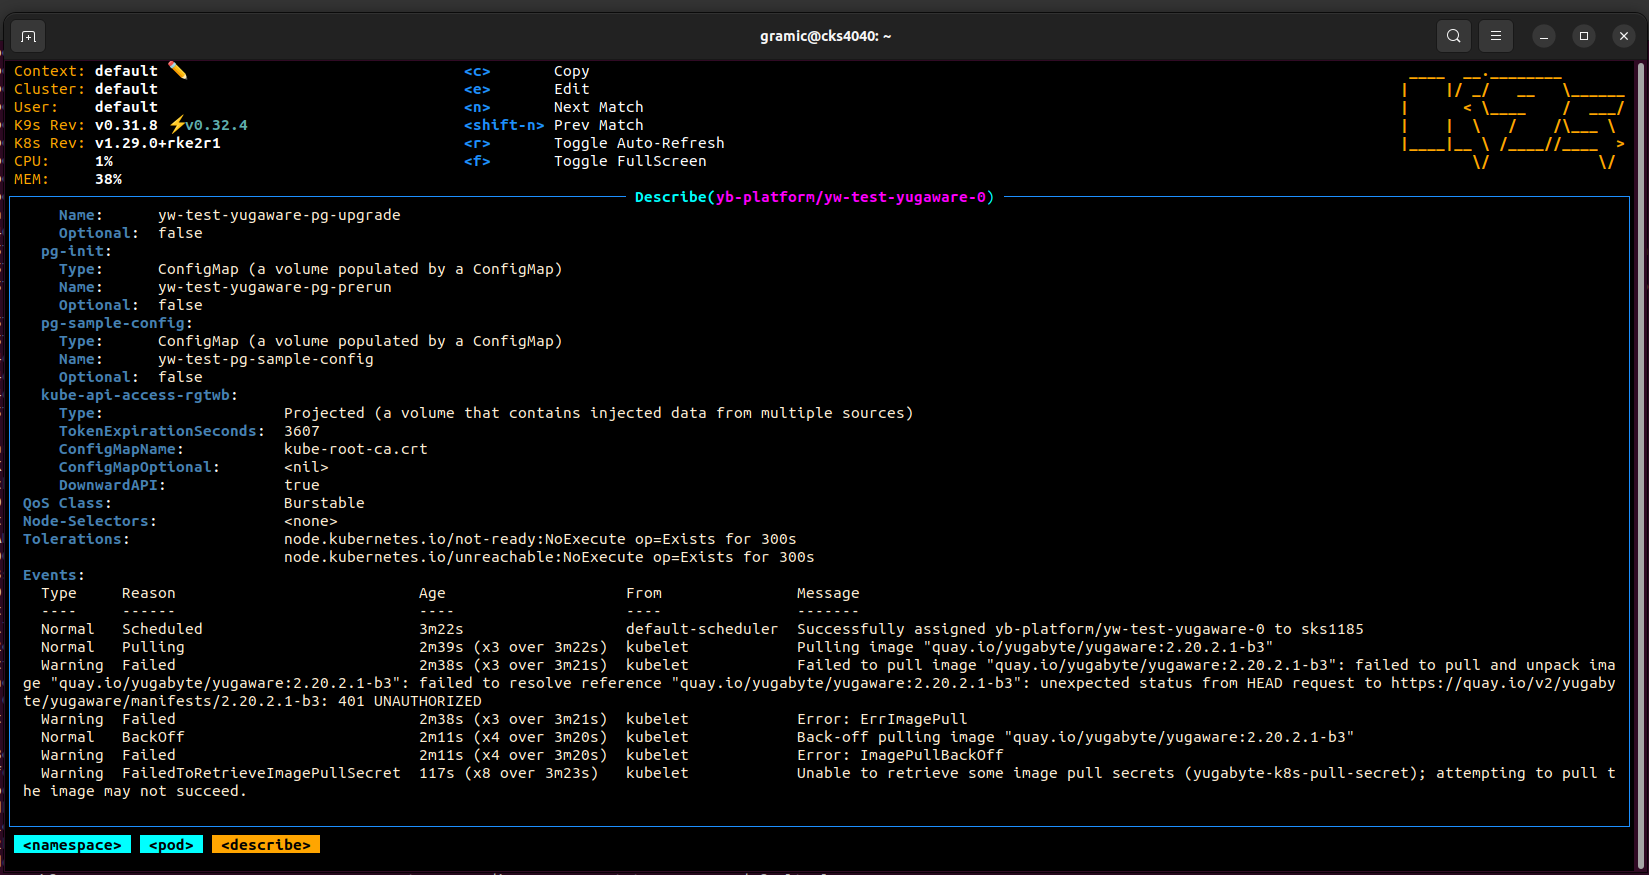
\includegraphics[width=1\linewidth]{source/implementation/evaluation/platforms/yugabytedb_pod_installation_subscription_interrup}
        \caption{yugabyteDB - Susbsription yugawre}
        \label{fig:yugabytedb_pod_installation_subscription_interrup}
    \end{figure}
\end{flushleft}
\begin{flushleft}
    Es stellte sich auch heraus, dass wenn man YugabyteDB 4 Cores pro Node zur Verfügung geben will (je zwei für den \texttt{master} und \texttt{tserver}),\\
    der Server mehr als 4 Cores haben muss.\\
    Andernfalls wird Kubernetes einen der beiden Pods nicht deployen, weil zuwenig Cores zur verfügung stehen.
\end{flushleft}
\begin{flushleft}
    Bei der konstelation \gls{rke2}, \Gls{Cilium} und \Gls{MetalLB}, muss nebst dem \texttt{IPAddressPool} auch ein \texttt{L2Advertisement} für den Pool gesetzt werden.\\
    Ansonsten kann die im YugabyteDB values.yaml gesetzte IP für den \texttt{tserver} von aussen nicht angesprochen werden:
    \lstset{style=gra_codestyle}
    \begin{lstlisting}[language=yaml, caption=metallb - Konfig YAML - Detail L2Advertisement,captionpos=b,label={lst:metallb-l2advertisement-setting},breaklines=true]
---
apiVersion: metallb.io/v1beta1
kind: L2Advertisement
metadata:
  name: l2adv
  namespace: metallb-system
spec:
  ipAddressPools:
  - distributed-sql
    \end{lstlisting}
    Dieses Problem ist schwer zu greifen und hat zwei Tage in Anspruch genommen, es zu Lösen.
    Die Vorschläge zum Lösen des Problems reichten von deakivieren von \texttt{kube-proxy} bis hin zu einer Migration zum \Gls{Cilium}-Loadb-Balancers.\\
    Mit diesem funktionierte dann nicht einmal mehr die Installation von yugabyteDB.\\
    Lösung brachte nur ein \texttt{GitHub}-Eintrag\cite{D4IZIEFN}, wo oben genannter Ansatz empfohlen wurde.
\end{flushleft}
\begin{flushleft}
    \paragraph{Konfiguration}
    Damit nicht der YugabyteDB Anywhere-Service installiert wird, muss das entsprechende Image gesetzt werden:
    \lstset{style=gra_codestyle}
    \begin{lstlisting}[language=yaml, caption=yugabyteDB - Helm Chart Manifest - Detail Image,captionpos=b,label={lst:yugabytedb-image-setting},breaklines=true]
...
Image:
  repository: "yugabytedb/yugabyte"
  tag: 2.20.2.1-b3
  pullPolicy: IfNotPresent
  pullSecretName: ""
...
    \end{lstlisting}

    Die StorageClass muss im \texttt{values.yaml} gesetzt werden, einmal für den \texttt{master} und einmal für den \texttt{tserver}
    \lstset{style=gra_codestyle}
    \begin{lstlisting}[language=yaml, caption=yugabyteDB - Helm Chart Manifest - Detail StorageClass,captionpos=b,label={lst:yugabytedb-storageclass-setting},breaklines=true]
...
storage:
  ephemeral: false  # will not allocate PVs when true
  master:
    count: 1
    size: 3Gi
    storageClass: "yb-storage"
  tserver:
    count: 1
    size: 3Gi
    storageClass: "yb-storage"
...
    \end{lstlisting}

    Dem node werden je 4 Cores zur verfügung gestellt.
    Zei für den \texttt{master} und zwei für den \texttt{tserver}.
    Beide erhalten 4GiB Memory:
    \lstset{style=gra_codestyle}
    \begin{lstlisting}[language=yaml, caption=yugabyteDB - Helm Chart Manifest - Detail Resources,captionpos=b,label={lst:yugabytedb-resources-setting},breaklines=true]
...
resource:
  master:
    requests:
      cpu: "1"
      memory: 2Gi
    limits:
      cpu: "1"
      ## Ensure the 'memory' value is strictly in 'Gi' or 'G' format. Deviating from these formats
      ## may result in setting an incorrect value for the 'memory_limit_hard_bytes' flag.
      ## Avoid using floating numbers for the numeric part of 'memory'. Doing so may lead to
      ## the 'memory_limit_hard_bytes' being set to 0, as the function expects integer values.
      memory: 2Gi
  tserver:
    requests:
      cpu: "1"
      memory: 4Gi
    limits:
      cpu: "1"
      ## Ensure the 'memory' value is strictly in 'Gi' or 'G' format. Deviating from these formats
      ## may result in setting an incorrect value for the 'memory_limit_hard_bytes' flag.
      ## Avoid using floating numbers for the numeric part of 'memory'. Doing so may lead to
      ## the 'memory_limit_hard_bytes' being set to 0, as the function expects integer values.
      memory: 4Gi
...
    \end{lstlisting}

    Die Shards, oder Tablets wie sie Yugabyte nennt, sollen auf allen drei Nodes repliziert werden:
    \lstset{style=gra_codestyle}
    \begin{lstlisting}[language=yaml, caption=yugabyteDB - Helm Chart Manifest - Detail Replika,captionpos=b,label={lst:yugabytedb-replica-setting},breaklines=true]
...
replicas:
  master: 3
  tserver: 3
  ## Used to set replication factor when isMultiAz is set to true
  totalMasters: 3
...
    \end{lstlisting}

    Wichtig ist auch, dass der \texttt{YSQL}-Dienst aktiv ist, damit PostgreSQL Abfragen abgesetzt werden können.\\
    Deshalb muss der Dienst aktiv sein und darf nicht deaktiviert werden:
    \lstset{style=gra_codestyle}
    \begin{lstlisting}[language=yaml, caption=yugabyteDB - Helm Chart Manifest - Detail Disable YSQL,captionpos=b,label={lst:yugabytedb-disableYsql-setting},breaklines=true]
...
# Disable the YSQL
disableYsql: false
...
    \end{lstlisting}

    Nun muss die Domain und die Service-Endpoints konfiguriert werden.\\
    Der Domainname bleibt vorerst \texttt{cluster.local} wie Default hinterlegt.\\
    Die Servicenamen und Ports werden nicht angetastet, wichtig ist die LoadBalancer-IP.\\
    Sie ist entsprechend der gewählten VirtualIP mit \texttt{10.0.20.106} zu setzen.

    \lstset{style=gra_codestyle}
    \begin{lstlisting}[language=yaml, caption=yugabyteDB - Helm Chart Manifest - Detail Domainname und Service-Endpoints,captionpos=b,label={lst:yugabytedb-domainname-serviceendpoints-setting},breaklines=true]
...
domainName: "cluster.local"

serviceEndpoints:
  - name: "yb-master-ui"
    type: LoadBalancer
    annotations: {}
    clusterIP: ""
    ## Sets the Service's externalTrafficPolicy
    externalTrafficPolicy: ""
    app: "yb-master"
    loadBalancerIP: ""
    ports:
      http-ui: "7000"

  - name: "yb-tserver-service"
    type: LoadBalancer
    annotations:
      metallb.universe.tf/loadBalancerIPs: 10.0.20.106
    clusterIP: ""
    ## Sets the Service's externalTrafficPolicy
    externalTrafficPolicy: ""
    app: "yb-tserver"
    loadBalancerIP: ""
    ports:
      tcp-yql-port: "9042"
      tcp-yedis-port: "6379"
      tcp-ysql-port: "5433"
...
    \end{lstlisting}
\end{flushleft}
\begin{flushleft}
    Beim Testen mit der höchsten Anzahl an Datensätzen zeigte sich, dass der \gls{local-path-provisioner} nicht sauber konfiguriert waren.\\
    Damit auf jedem Node die Persistence Volume Claims ausgeführt werden, müssen sie deklariert werden und in den StorageClass-Manifesten auch hinterlegt werden.\\
    Genauer muss in der \texttt{nodePathMap} folgende konfiguration vorgenommen werden:
\lstset{style=gra_codestyle}
\begin{lstlisting}[language=yaml, caption=local-path-provisioner nodePathMap,captionpos=b,label={lst:local-path-provisioner_nodePathMap},breaklines=true]
...
                "nodePathMap":[
                {
                        "node":"DEFAULT_PATH_FOR_NON_LISTED_NODES",
                        "paths":["<Lokaler Pfad>"]
                },
                {
                        "node":"<Nodename>",
                        "paths":["<Lokaler Pfad>"]
                },
...
\end{lstlisting}
    Hier ein Beispiel wie es mit den grossen Volumes aussieht:
\lstset{style=gra_codestyle}
\begin{lstlisting}[language=yaml, caption=local-path-provisioner nodePathMap Beispiel,captionpos=b,label={lst:local-path-provisioner_nodePathMap-exampl},breaklines=true]
...
                "nodePathMap":[
                {
                        "node":"DEFAULT_PATH_FOR_NON_LISTED_NODES",
                        "paths":["/srv/data/local-path-provisioner"]
                },
                {
                        "node":"sks1183",
                        "paths":["/srv/data/local-path-provisioner"]
                },
                {
                        "node":"sks1184",
                        "paths":["/srv/data/local-path-provisioner"]
                },
                {
                        "node":"sks1185",
                        "paths":["/srv/data/local-path-provisioner"]
                }
                ]
...
\end{lstlisting}
    Wird dies nicht gemacht, so wird auf den Default-Path geschrieben.\\
    Das ist zufällig und hat dann zur Folge, dass alle Volumes auf einem Node präsentiert werden.\\
    Was sehr schnell logischerweise dazu führt, dass zuwenig Diskspace vorhanden ist.\\
    Bei YugabyteDB kommt noch dazu, dass es zu Konflikten beim Schreiben von Blocks kommt.
\end{flushleft}
\begin{flushleft}
    Damit die Persistence Volumes sauber präsentiert werden, muss in der StorageClass die \texttt{nodeAffinity} gesetzt werden.\\
    Hier als Beispiel mit den Nodes \texttt{sks1183}, \texttt{sks1184} und \texttt{sks1185}:
\lstset{style=gra_codestyle}
\begin{lstlisting}[language=yaml, caption=yugabyteDB - StorageClass nodeAffinity,captionpos=b,label={lst:yugabytedb-storageclass_example},breaklines=true]
  nodeAffinity:
    required:
      nodeSelectorTerms:
      - matchExpressions:
        - key: kubernetes.io/hostname
          operator: In
          values:
          - sks1183
          - sks1184
          - sks1185
\end{lstlisting}
    \begin{warning}
        \textbf{hostPath}\\
        Der \texttt{hostPath} bei der StorageClass muss der gleiche sein, wie der Pfad im Node des nodePathMap von \gls{local-path-provisioner}.
        Auch sollten die Pfade auf allen Nodes gleich sein.
    \end{warning}
\end{flushleft}
\begin{flushleft}
    Die Problematik mit dem \texttt{nodePathMap} und der \texttt{nodeAffinity} auf der StorageClass hat auch rund zwei Arbeitstage in Anspruch genommen.
\end{flushleft}
    \subsubsection{Stackgres mit Citus}
\begin{flushleft} 
Stackgres ist eine PostgreSQL Implementation die dafür vorgesehenen ist, in einem Kubernetes Cluster betrieben zu werden.
\end{flushleft} 
\begin{flushleft}
An sich wäre Stackgres nur eine Implementation von Patroni in Kubernetes inkl. Load Balancer.\\
Nun kommt das Citus-Plugin ins spiel, welches aus einer jeden Monolithischen, Klassischen PostgreSQL Installation eine Distributed SQL Umgebung macht.////
Citus wiederum ist in den Microsoft Konzern eingebettet
\end{flushleft}

\begin{flushleft}
    \paragraph{Architektur}
    \begin{flushleft}
        \subparagraph{Citus Coordinator und Workers}
        \begin{figure}[H]
            \centering
            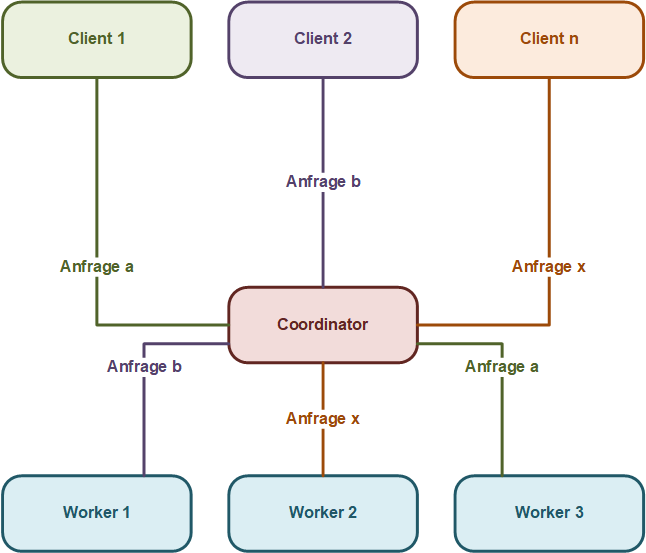
\includegraphics[width=0.75\linewidth]{source/implementation/evaluation/postgresql_ha_solutions/stackgres/citus_coordinator_worker}
            \caption{Citus - Coordinator und Workers}
            \label{fig:citus_coordinator_worker}
        \end{figure}
    \end{flushleft}
    \begin{flushleft}
        \subparagraph{Citus Sharding}
        Citus bietet zwei Sharding-Modelle an.
        \begin{flushleft}
            \textbf{Row-based sharding}
            Beim diesen sharding werden Tabellen anhand einer Distribution Column aufgeteilt. \cite{2Y5FA36C, FDUUL9IM}
        \end{flushleft}
        \begin{flushleft}
            \textbf{Schema-based sharding}
        \end{flushleft}
    \end{flushleft}
\end{flushleft}
\begin{flushleft}
    \paragraph{Maintenance}
    Bei Stackgres gab es im letzten Monat keine wirkliche Bewegung:
    \begin{figure}[H]
        \centering
        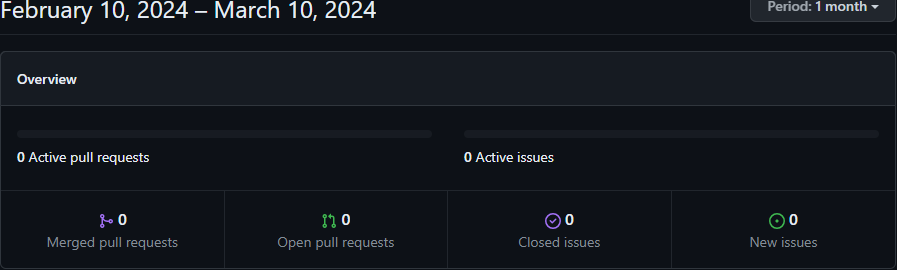
\includegraphics[width=0.75\linewidth]{source/implementation/evaluation/postgresql_ha_solutions/insights/stackgres_citus/pulse_ongres_stackgres}
        \caption{Stackgres - Pulse}
        \label{fig:pulse_ongres_stackgres}
    \end{figure}
    Anders sieht es bei Citus aus, die Firma die mittlerweile zu Microsoft gehört, schliesst Issues rasch und hat eine verhältnissmässig hohe Requstrate:
    \begin{figure}[H]
        \centering
        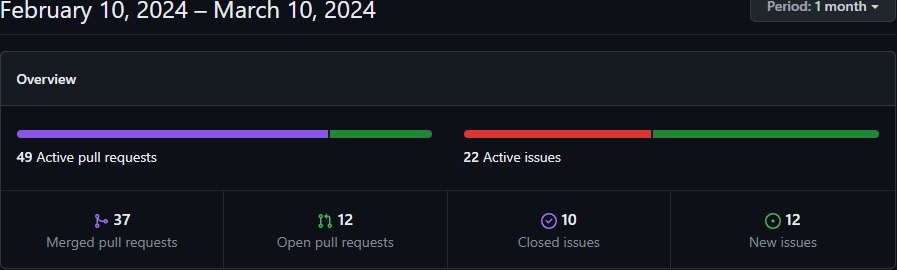
\includegraphics[width=0.75\linewidth]{source/implementation/evaluation/postgresql_ha_solutions/insights/stackgres_citus/pulse_citusdata_citus}
        \caption{Citus - Pulse}
        \label{fig:pulse_citusdata_citus}
    \end{figure}

    Bei Stackgres wird sehr viel Code hinzugefügt oder gelöscht, beim älteren Citus wurden weniger änderungen verzeichnet:
    \begin{figure}[H]
        \centering
        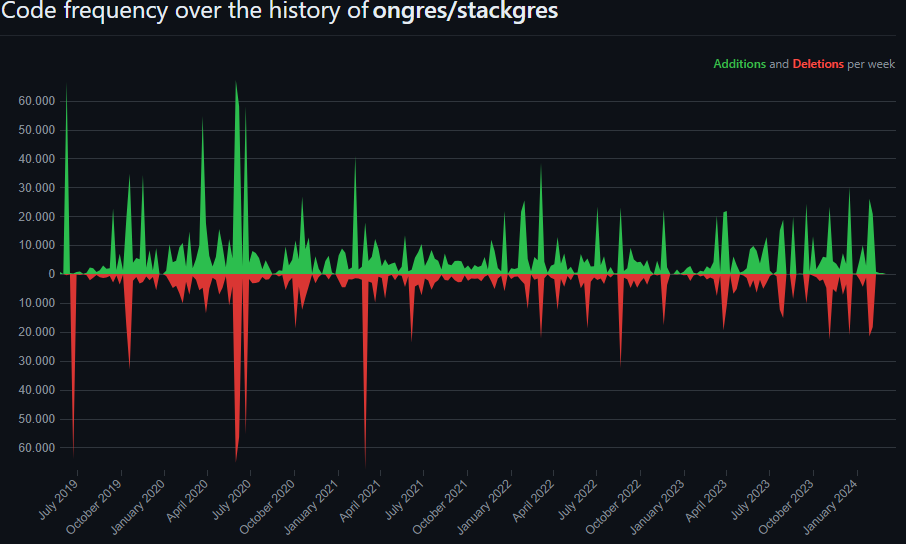
\includegraphics[width=0.75\linewidth]{source/implementation/evaluation/postgresql_ha_solutions/insights/stackgres_citus/code_frequency_ongres_stackgres}
        \caption{Stackgres - Code Frequency}
        \label{fig:code_frequency_ongres_stackgres}
    \end{figure}
    \begin{figure}[H]
        \centering
        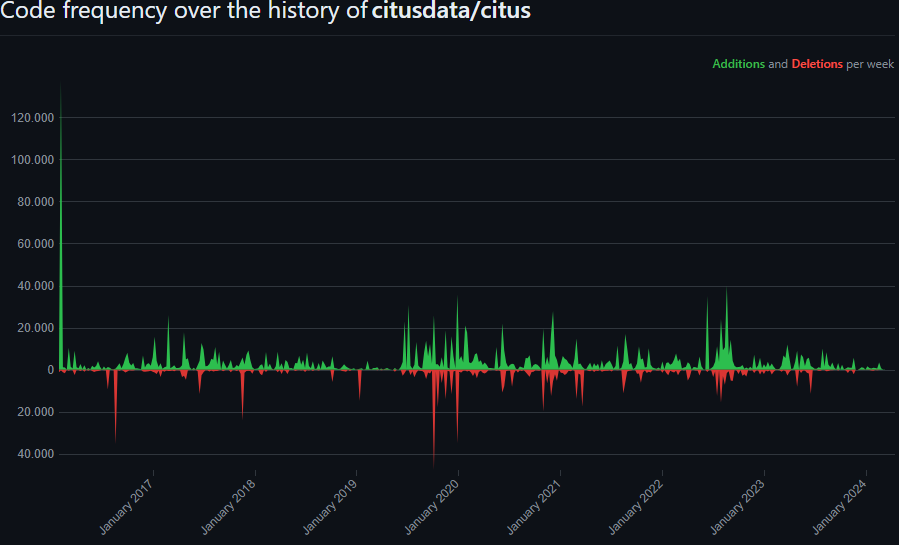
\includegraphics[width=0.75\linewidth]{source/implementation/evaluation/postgresql_ha_solutions/insights/stackgres_citus/code_frequency_citusdata_citus}
        \caption{Citus - Code Frequency}
        \label{fig:code_frequency_citusdata_citus}
    \end{figure}

    Citus legt einen hohen Stellenwert auf die Community-Standars, Stackgres selbst schneidet hier nur Mittelmässig ab:
    \begin{figure}[H]
        \centering
        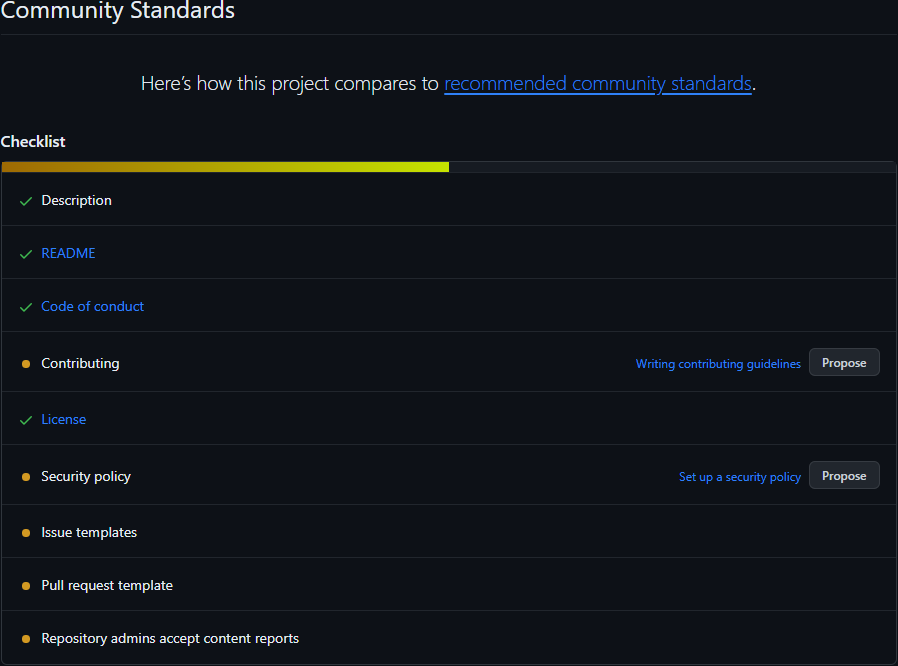
\includegraphics[width=0.75\linewidth]{source/implementation/evaluation/postgresql_ha_solutions/insights/stackgres_citus/stackgres_community_standards}
        \caption{Stackgres - Community Standards}
        \label{fig:stackgres_community_standards}
    \end{figure}
    \begin{figure}[H]
        \centering
        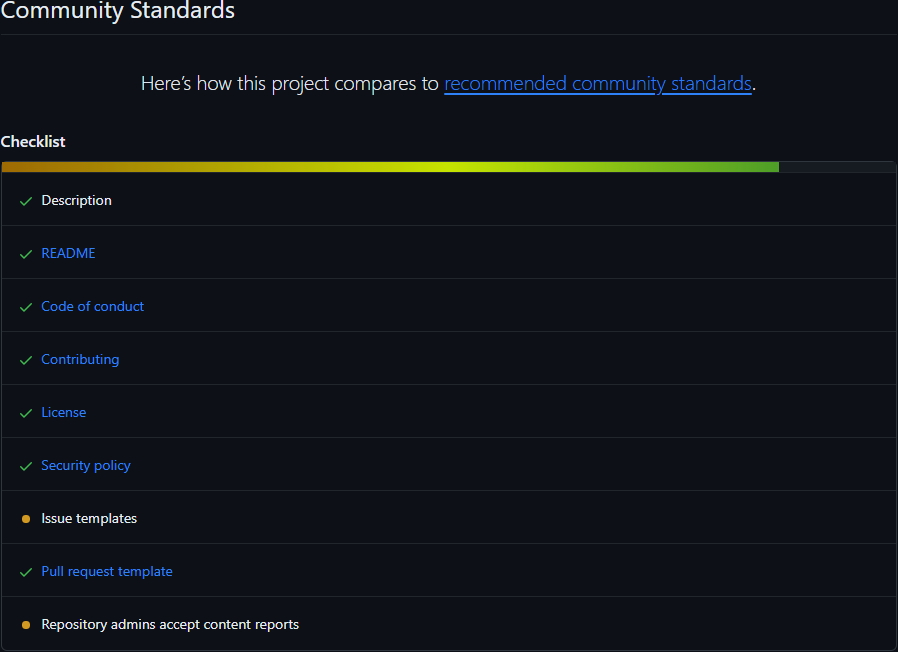
\includegraphics[width=0.75\linewidth]{source/implementation/evaluation/postgresql_ha_solutions/insights/stackgres_citus/citus_community_standards}
        \caption{Citus - Community Standards}
        \label{fig:citus_community_standards}
    \end{figure}

    Die Stackgres Constributors pflegen aktiv Additions ein, löschen Regelmässig und Commiten ebenfalls auf die main-Branch.
    Citus, dessen Repository länger Commited wird, hat weniger bewegung auf die main-Branch.
    \begin{figure}[H]
        \centering
        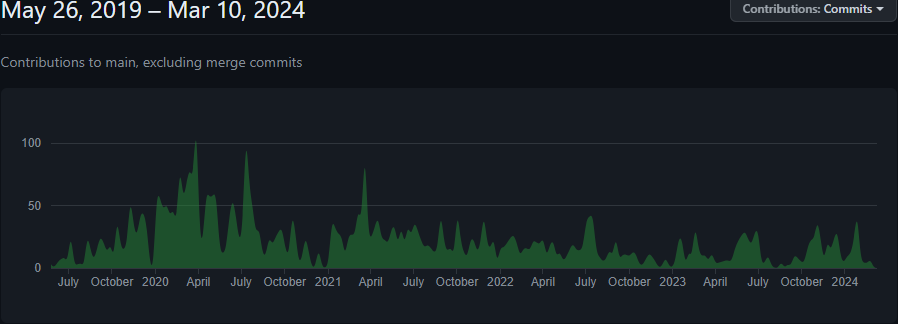
\includegraphics[width=0.75\linewidth]{source/implementation/evaluation/postgresql_ha_solutions/insights/stackgres_citus/contributors_commits_ongres_stackgres}
        \caption{Stackgres - Contributors Commits}
        \label{fig:contributors_commits_ongres_stackgres}
    \end{figure}
    \begin{figure}[H]
        \centering
        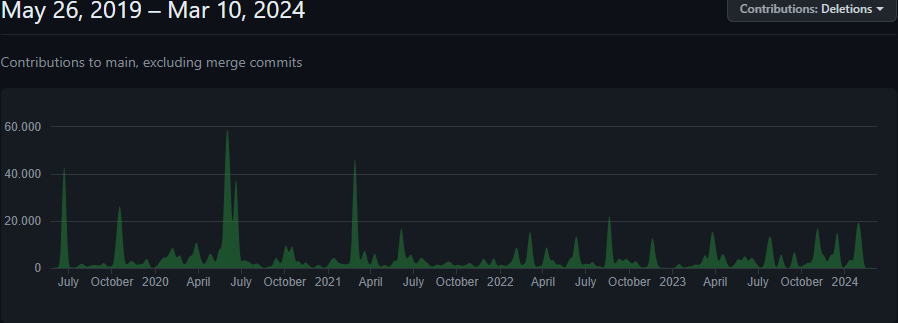
\includegraphics[width=0.75\linewidth]{source/implementation/evaluation/postgresql_ha_solutions/insights/stackgres_citus/contributors_deletations_ongres_stackgres}
        \caption{Stackgres - Contributors Deletations}
        \label{fig:contributors_deletations_ongres_stackgres}
    \end{figure}
    \begin{figure}[H]
        \centering
        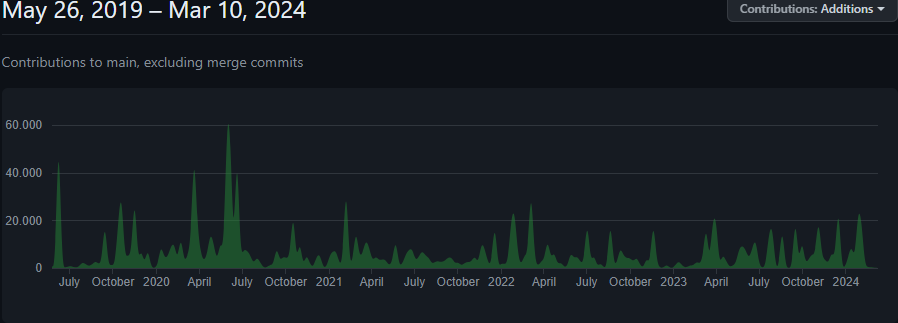
\includegraphics[width=0.75\linewidth]{source/implementation/evaluation/postgresql_ha_solutions/insights/stackgres_citus/contributors_addition_ongres_stackgres}
        \caption{Stackgres - Contributors Additions}
        \label{fig:contributors_addition_ongres_stackgres}
    \end{figure}
    \begin{figure}[H]
        \centering
        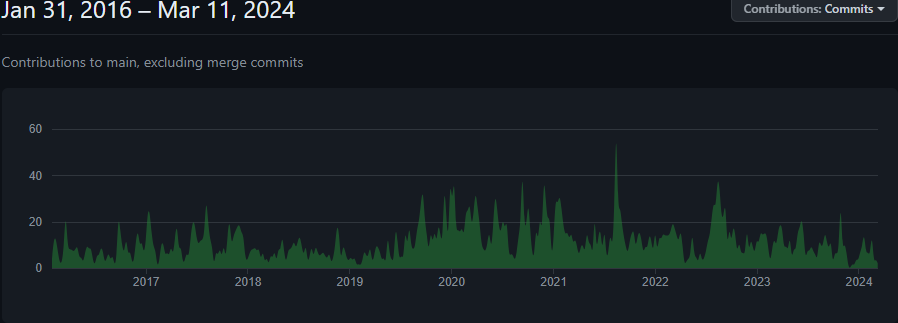
\includegraphics[width=0.75\linewidth]{source/implementation/evaluation/postgresql_ha_solutions/insights/stackgres_citus/contributors_commits_citusdata_citus}
        \caption{Citus - Contributors Commits}
        \label{fig:contributors_commits_citusdata_citus}
    \end{figure}
    \begin{figure}[H]
        \centering
        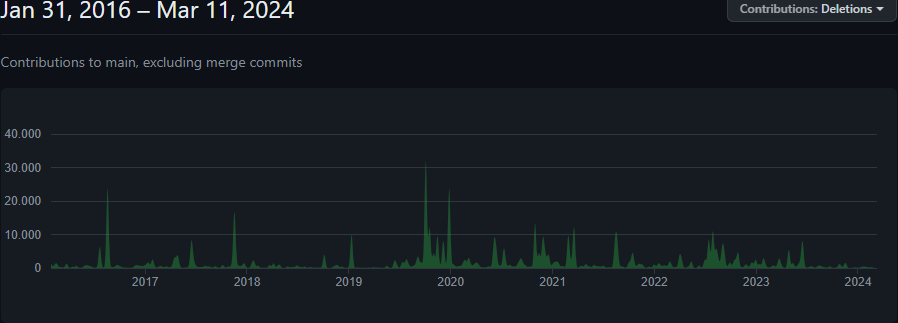
\includegraphics[width=0.75\linewidth]{source/implementation/evaluation/postgresql_ha_solutions/insights/stackgres_citus/contributors_deletations_citusdata_citus}
        \caption{Citus - Contributors Deletations}
        \label{fig:contributors_deletations_citusdata_citus}
    \end{figure}
    \begin{figure}[H]
        \centering
        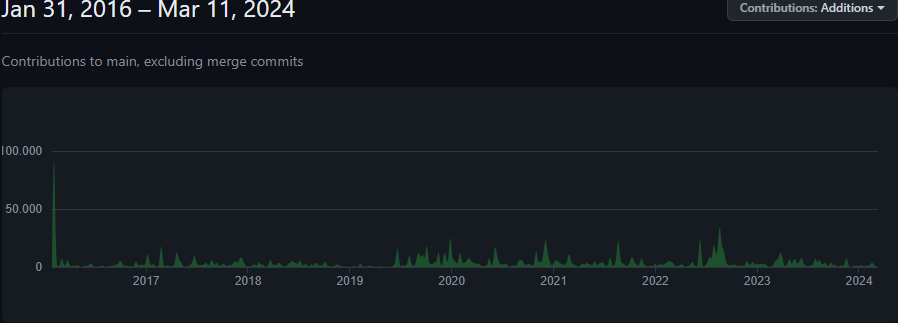
\includegraphics[width=0.75\linewidth]{source/implementation/evaluation/postgresql_ha_solutions/insights/stackgres_citus/contributors_additions_citusdata_citus}
        \caption{Citus - Contributors Additions}
        \label{fig:contributors_additions_citusdata_citus}
    \end{figure}

    Gerade Ende Januar gab es bei Stackgres eine grössere Anzahl Commits, anhand der statistik wird ersichtlich, dass i.d.R. einmal pro Monat grössere Mengen an Commits eingespielt werden.
    Bei Citus gibt es ebenfalls Regelmässig grössere Mengen an Commits, allerdings scheint bei citusdata mehr mit kürzeren Sprints gearbeitet zu werden als bei ongres denn die Commits sind Regelmässiger:
    \begin{figure}[H]
        \centering
        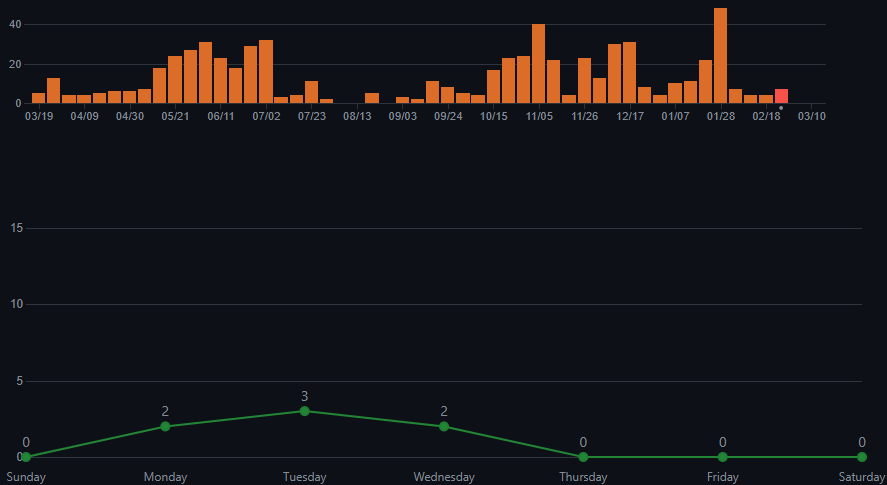
\includegraphics[width=0.75\linewidth]{source/implementation/evaluation/postgresql_ha_solutions/insights/stackgres_citus/commit_activity_ongres_stackgres}
        \caption{Stackgres - Commit Activity}
        \label{fig:commit_activity_ongres_stackgres}
    \end{figure}
    \begin{figure}[H]
        \centering
        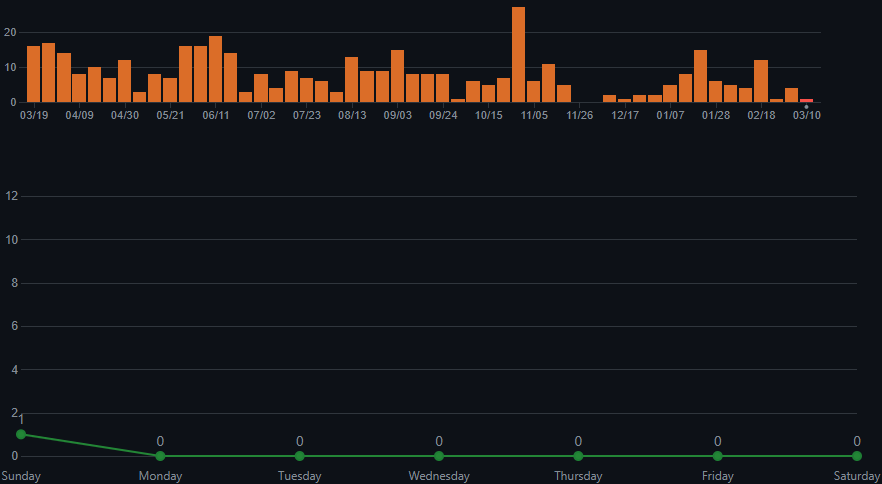
\includegraphics[width=0.75\linewidth]{source/implementation/evaluation/postgresql_ha_solutions/insights/stackgres_citus/commit_activity_citusdata_citus}
        \caption{Citus - Commit Activity}
        \label{fig:commit_activity_citusdata_citus}
    \end{figure}

    In letzter Zeit haben nur ongres, der Entwickler von Stackgres, als auch citusdata, grössere Commits auf das Repository gefahren.
    Andere grössere Entwickler wie EnterpriseDB sind abwesend.
    \begin{figure}[H]
        \centering
        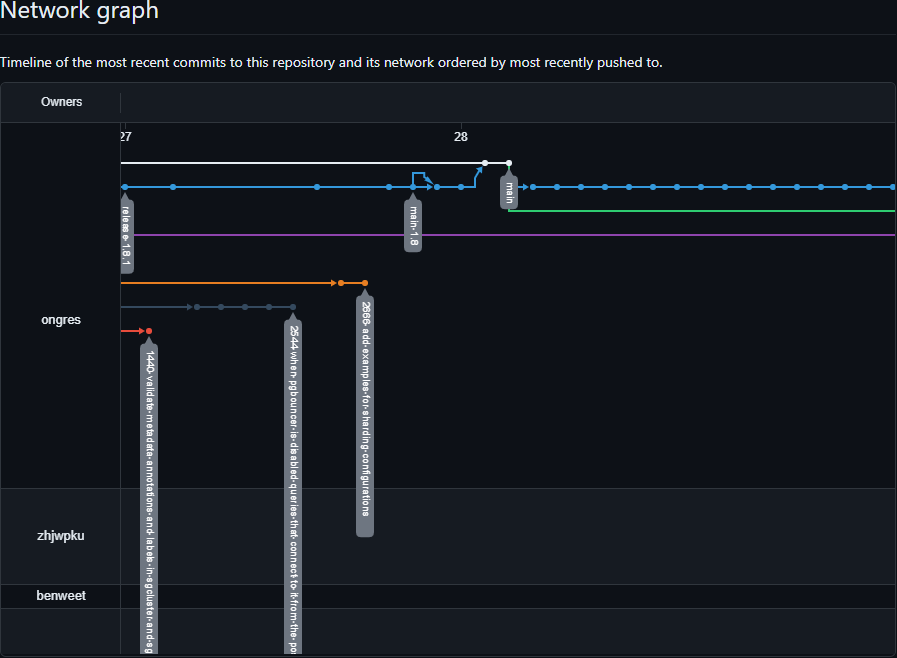
\includegraphics[width=0.75\linewidth]{source/implementation/evaluation/postgresql_ha_solutions/insights/stackgres_citus/network_graph_ongres_stackgres}
        \caption{Stackgres - Network Graph}
        \label{fig:network_graph_ongres_stackgres}
    \end{figure}
    \begin{figure}[H]
        \centering
        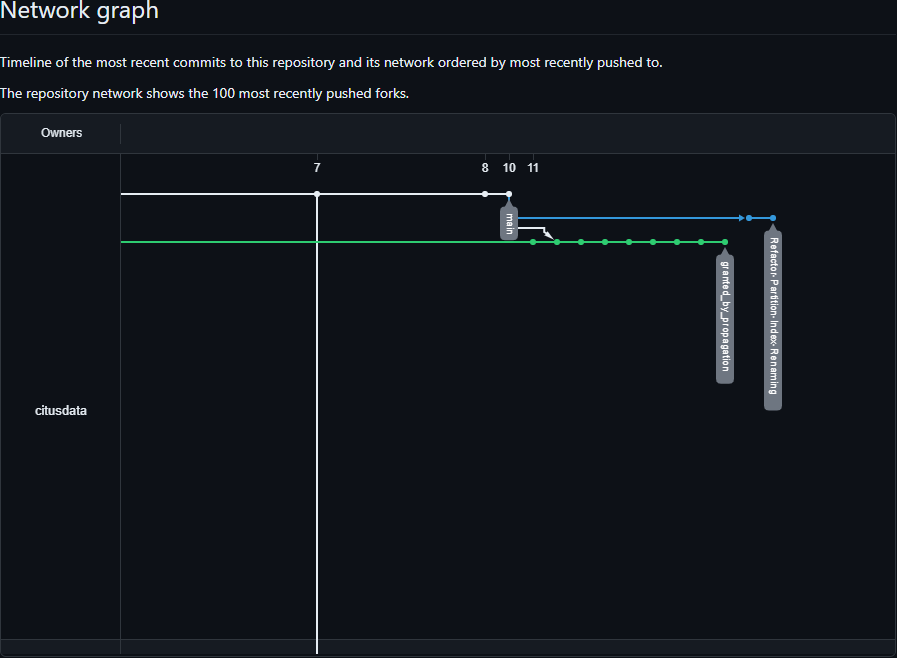
\includegraphics[width=0.75\linewidth]{source/implementation/evaluation/postgresql_ha_solutions/insights/stackgres_citus/network_graph_citusdata_citus}
        \caption{Citus - Network Graph}
        \label{fig:network_graph_citusdata_citus}
    \end{figure}

\end{flushleft}

    %! Author = itgramic
%! Date = 05.01.24

% Preamble
\newpage
\section{Disposition}
\label{chap:disposition}
%\begin{flushleft}
%    \begin{figure}[H]
%        \centering
%%        
\includegraphics[width=1\linewidth]{source/appendix/Michael_Graber_Disposition_Diplomarbeit_2023_2024}
%        
\includepdf[pages={1-},scale=0.75]{source/appendix/Michael_Graber_Disposition_Diplomarbeit_2023_2024}
%        \caption{Disposition}
%        \label{fig:disposition}
%    \end{figure}

\includepdf[pages={1-},scale=0.75]{source/appendix/Michael_Graber_Disposition_Diplomarbeit_2023_2024}
%\caption{Disposition}
%\label{fig:disposition}
\captionof{figure}{Disposition}
%\end{flushleft}

\end{appendix}



\end{document}
